%!TEX root = P231_notes.tex

\documentclass[12pt]{article}
%!TEX root = P231_notes.tex

%%%%%%%%%%%%%%%%%%%%%%%%%%
%%%  COMMON PACKAGES  %%%%
%%%%%%%%%%%%%%%%%%%%%%%%%%

\usepackage{amsmath}
\usepackage{amssymb}
\usepackage{amsfonts}
\usepackage{graphicx}
\usepackage[utf8]{inputenc}			% inspire bibs
\usepackage{aas_macros}				% ads bibs
%\usepackage{amsthm}

%%%%%%%%%%%%%%%%%%%%%%%%%%%%%%%%%
%%%  UNUSUAL PACKAGES        %%%%
%%%  Uncomment as necessary. %%%%
%%%%%%%%%%%%%%%%%%%%%%%%%%%%%%%%%

%% MATH AND PHYSICS SYMBOLS
%% ------------------------
\usepackage{slashed}				% \slashed{k}
\usepackage{mathrsfs}				% Weinberg-esque letters
\usepackage{bbm}					% \mathbbm{1} conflict: XeLaTeX 
\usepackage{cancel}					
\usepackage[normalem]{ulem} 		% for \sout
%\usepackage{youngtab}	    		% Young Tableaux


%% CONTENT FORMAT AND DESIGN
%% -------------------------
\usepackage[dvipsnames]{xcolor}
\usepackage[hang,flushmargin]{footmisc} % no footnote indent

\usepackage{fancyhdr}		% preprint number
\usepackage{lipsum}			% block of text 
\usepackage{framed}			% boxed remarks
\usepackage{subcaption}		% subfigures
\usepackage{cite}			% group cites
\usepackage{xspace}			% macro spacing

\usepackage{marginnote} 


%% TABLES IN LaTeX
%% ---------------
\usepackage{booktabs}		% professional tables
%\usepackage{nicefrac}		% fractions in tables,
%\usepackage{multirow}		% multirow elements in a table
%\usepackage{arydshln}		% dashed lines in arrays

%% Other Packages and Notes
%% ------------------------
\usepackage[font=small]{caption} % caption font is small
\usepackage{float}         % for strict placement e.g. [H]
 



%%%%%%%%%%%%%%%%%%%%%%%%%%%%%%
%%%  DOCUMENT PROPERTIES  %%%%
%%%%%%%%%%%%%%%%%%%%%%%%%%%%%%

% \usepackage[margin=2cm]{geometry}   % margins
\usepackage[
  top=2.5cm, 
  bottom=2.5cm, 
  outer=2.5cm,            % size of margin
  inner=2.5cm,              % size of opposite margin
  heightrounded, 
  marginparwidth=1.5cm,   % less than outer
  marginparsep=.2cm%    % between text and margin note
  ]{geometry}
%% https://en.wikibooks.org/wiki/LaTeX/Footnotes_and_Margin_Notes#Margin_Notes
\graphicspath{{figures/}}			% figure folder
\numberwithin{equation}{section}    % set equation numbering


%% References in two columns, smaller
%% http://tex.stackexchange.com/questions/20758/
\usepackage{multicol}
\usepackage{etoolbox}
\usepackage{relsize}
\patchcmd{\thebibliography}
  {\list}
  {\begin{multicols}{2}\smaller\list}
  {}
  {}
\appto{\endthebibliography}{\end{multicols}}


% Change list spacing (instead of package paralist)
% from: http://en.wikibooks.org/wiki/LaTeX/List_Structures#Line_spacing
\let\oldenumerate\enumerate
\renewcommand{\enumerate}{
  \oldenumerate
  \setlength{\itemsep}{3pt}
  \setlength{\parskip}{0pt}
  \setlength{\parsep}{0pt}
}

\let\olditemize\itemize
\renewcommand{\itemize}{
  \olditemize
  \setlength{\itemsep}{1pt}
  \setlength{\parskip}{0pt}
  \setlength{\parsep}{0pt}
}


%%%%%%%%%%%%%%%%%%%%%%%%%%%
%%%  (RE)NEW COMMANDS  %%%%
%%%%%%%%%%%%%%%%%%%%%%%%%%%

%% FOR `NOT SHOUTING' CAPS (e.g. acronyms)
%% ---------------------------------------
\newcommand{\acro}[1]{\textsc{\MakeLowercase{#1}}}    
\usepackage{scalefnt}
\newcommand\acronum[2][0.85]{{\scalefont{#1}#2}} 

%% COMMON PHYSICS MACROS
%% ---------------------
\renewcommand{\tilde}{\widetilde}   % tilde over characters
\renewcommand{\vec}[1]{\mathbf{#1}} % vectors are boldface
\newcommand{\dbar}{d\mkern-6mu\mathchar'26}    % for d/2pi
\newcommand{\ket}[1]{\left|#1\right\rangle}    % <#1|
\newcommand{\bra}[1]{\left\langle#1\right|}    % |#1>
\newcommand{\mat}[3]{#1^{#2}_{\phantom{#2}#3}}    % <#1|
\renewcommand{\text}{\textnormal} % text in equations 

%% THEOREM ENVIRONMENT
%% -------------------
\newtheorem{exercise}{Exercise}[section]
\newtheorem{example}{Example}[section]

%% COMMANDS FOR TEMPORARY COMMENTS
%% -------------------------------
\newcommand{\comment}[2]{\textcolor{red}{[\textbf{#1} #2]}}
\newcommand{\flip}[1]{{
	\color{green!50!black} \footnotesize [\textbf{\textsf{Flip}}: \textsf{#1}]
	}}

% \newcommand{\lecdate}[1]{\marginnote{\footnotesize\color{blue!50!black}{\textsf{#1}}}}
\newcommand{\lecdate}[1]{}


%% COMMANDS FOR TOP-MATTER
%% -----------------------
\newcommand{\email}[1]{\href{mailto:#1}{#1}}
\newenvironment{institutions}[1][2em]{\begin{list}{}{\setlength\leftmargin{#1}\setlength\rightmargin{#1}}\item[]}{\end{list}}


%% COMMANDS FOR LATEXDIFF
%% ----------------------
%% see http://bit.ly/1M74uwc
\providecommand{\DIFadd}[1]{{\protect\color{blue}#1}} %DIF PREAMBLE
\providecommand{\DIFdel}[1]{{\protect\color{red}\protect\scriptsize{#1}}}

%% REMARK: use latexdiff option --allow-spaces
%% for \frac, ref: http://bit.ly/1iFlujR


%%%%%%%%%%%%%%%%%%%
%%%  HYPERREF  %%%%
%%%%%%%%%%%%%%%%%%%

%% This package has to be at the end; can lead to conflicts
\usepackage[
	colorlinks=true,
	citecolor=green!50!black,
	linkcolor=NavyBlue!75!black,
	urlcolor=green!50!black,
	hypertexnames=false]{hyperref}


%%%%%%%%%%%%%%%%%%%%%
%%%  TITLE DATA  %%%%
%%%%%%%%%%%%%%%%%%%%%

%% PREPRINT NUMBER USING fancyhdr
%% Don't forget to set \thispagestyle{firststyle}
%% ----------------------------------------------
\renewcommand{\headrulewidth}{0pt} 	% no separator
\setlength{\headheight}{15pt} 		% min to avoid fancyhdr warning
\fancypagestyle{firststyle}{
	\rhead{\footnotesize%
	\texttt{UCR-P231-FLIP-F2020}%
	}}

%% TOC overwrites fancyhdr, here's a fix
%% http://tex.stackexchange.com/questions/167828/
\usepackage{etoc}
\renewcommand{\etocaftertitlehook}{\pagestyle{plain}}
\renewcommand{\etocaftertochook}{\thispagestyle{firststyle}}

\begin{document}

%\thispagestyle{empty}		% default if no preprint #
\thispagestyle{firststyle} 	% to include preprint
%% I think this may screw up pdfsync on the first page

\begin{center}
	
	{\large \acronum{P231:}}
    {\Large \bf Mathematical Methods in Graduate Physics}

    \vskip .7cm

%% SINGLE AUTHOR FORMAT
%% --------------------
	\textbf{Flip Tanedo} \\
	\texttt{\footnotesize \email{flip.tanedo@ucr.edu}}

	\vspace{-1em}
    \begin{institutions}[1.5cm]
    \footnotesize
    {\it 
	    Department of Physics \& Astronomy, 
	    University of  California, Riverside, 
	    {CA} 92521	    
	    }    
    \end{institutions}


\end{center}




%%%%%%%%%%%%%%%%%%%%%
%%%  ABSTRACT    %%%%
%%%%%%%%%%%%%%%%%%%%%

\begin{abstract}
\noindent 
This is a crash course on mathematical methods necessary to succeed in the first-year physics graduate curriculum at \acro{UC} Riverside. 
%
The focus is how to solve differential equations using Green's functions.
\end{abstract}



\small
\setcounter{tocdepth}{2}
\tableofcontents
\normalsize
%\clearpage


%%%%%%%%%%%%%%%%%%%%%
%%%  THE CONTENT  %%%
%%%%%%%%%%%%%%%%%%%%%

\input{Lec-00-intro}
%!TEX root = P231_notes.tex

\subsection{Physics versus Mathematics}
\lecdate{lec~02}


Let’s make one point clear:
\begin{align}
  \text{Physics} \neq \text{Mathematics} \ .
\end{align}
This is a truth in many different respects\footnote{The astronomer Fritz Zwicky would perhaps call this a \emph{spherical truth}; no matter how you look at it, the statement is still true.}:
\begin{itemize}
	\item Physicists are rooted in experimental results\footnote{Even theorists? \emph{especially} theorists.}. 
	
	\item Physicists Taylor expand to their hearts’ content---sometimes even when the expansion is not formally justified\footnote{\url{https://johncarlosbaez.wordpress.com/2016/09/21/struggles-with-the-continuum-part-6/}}.

	\item Physicists use explicit coordinates, mathematicians abhor this.  Even worse, we pick a basis and decorate every tensor with indices\footnote{Those who are not trained may be intimidated by physics because of all the indices we use. Ironically, physicists are often intimidated by mathematics because of the conspicuous absence of any indices.}.

	\item Physicists seek to uncover a truth about \emph{this} universe.
\end{itemize}

% We use mathematical formalism to describe the universe. Sometimes the formalism that we need even spurs on developments in formal mathematics. However, let us be clear that our descriptions of the universe are \emph{mathematical models}. Our models have limits of validity: where they are tested, where they break down. 

\subsection{The most important binary relation}


When we write equations, the symbol that separates the left-hand side from the right-hand side is a binary relation. We use binary relations like $=$ or $\neq$. Sometimes to make a point we’ll write $\cong$ or $\equiv$ or $\dot =$ to mean something like `definition’ or `tautologically equivalent to’ or some other variant of \emph{even more equal than equal}. 

As physicists the most important binary relation is none of those things\footnote{I thank Yuval Grossman for emphasizing this. Unrelated: \url{https://xkcd.com/2343/}}. Usually what we really care about is in $\sim$.\footnote{I use this the same way as $\propto$, which is completely different from `approximately,’ $\approx$.} This tells how how something \emph{scales}. If I double a quantity on the right-hand side, how does the quantity on the left-hand side scale? Does it depend linearly? Quadratically? Non-linearly? The answer encodes something important about the underlying physics of the system. It's the reason why \emph{imagine the cow is a sphere} is a popular punchline in a joke about physicists. 


By the way, implicit in this is the idea that in this class, we will not care about stray factors of 2. As my adviser used to say, if you’re worried about a factor of 2, then your additional homework is to figure out that factor of 2.\footnote{That being said, you're reading these notes and find an error, do let me know about it.} 

\subsection{Units}

There is another way in which physics is different from mathematics. It is far more prosaic. \emph{Quantities in physics have units}. We don’t just deal with numbers, we deal with kilograms, electron volts, meters. It turns out that dimensional analysis is a big part of what we do as physicists. 

\input{Lec-02-dimensional-analysis}
\input{Lec-03-linear-algebra}
%!TEX root = P231_notes.tex

\section{Function Space}
\lecdate{lec~04}

\textbf{Function spaces} are vector spaces where the vectors are functions. We introduced `histogram space' in Section~\ref{sec:histogramspace} as a crude model of a finite dimensional function spaces. An alternative finite dimensional model is the space of polynomials up to some degree, which we introduced in Section~\ref{sec:derivatives}. Our models of nature are typically continuous\footnote{This does not mean that nature is fundamentally continuous. There is a deep sense in which our models are valid whether or not nature is continuous so long as any granularity is smaller than our experimental probes.}. This requires \emph{infinite} dimensional function spaces, or Hilbert spaces.

\subsection{The Green's Function Problem in Function Space}

The Green's function can be defined by analogy to the finite-dimensional inverse transformation. The finite-dimensional linear system $A\vec v = \vec w$ can be solved by applying the inverse transformation $A^{-1}$ in the same way that the continuum (infinite-dimensional) system $\mathcal O \psi(x) = s(x)$ can be solved with the Green's function $G(x,y)$ of the operator $\mathcal O$:
\begin{align}
	v^i &= \sum_i \mat{\left(A^{-1}\right)}{i}{j} w^j
	&\Rrightarrow
	&
	&
	\psi(x) &= \int  dy\, G(x,y) s(y) \ .
	\label{eq:def:of:function:space:Greens:function}
\end{align}
We've explicitly written out the sum over the dummy index $i$ to emphasize the analogy to the integration over the dummy variable $y$. The arguments of the functions play the role of `continuum indices.'

\subsection{Differential Operators}

Linear transformations on function space are differential operators. In principle you can imagine linear transformations that are not differential operators, for example a finite translation. However, because our models of nature are typically \emph{local} and \emph{causal}, the linear transformations that we obtain from physical models are differential operators\footnote{This is not to say that finite transformations are somehow not permitted. The dynamics that govern our models of nature, however, only dictate how information is transmitted infinitesimally in space and time. Propagation forward in time by some finite interval is described by the exponentiation of infinitesimal forward time translations. This is, of course, why the time-translation operator in quantum mechanics is $e^{i\hat H t}$, where the Hamiltonian $H$ is described as a local function with perhaps one or two derivative operators.}. 

Let's write a general differential operator as:
\begin{align}
	\mathcal O = 
	p_0(x) 
	+ p_1(x) \frac{d}{dx}
	+ p_2(x) \left(\frac{d}{dx}\right)^2
	+ \cdots
	\label{eq:differential:operator}
\end{align}
where the $p_i(x)$ are polynomials. Sometimes we will write this as $\mathcal O_x$ to make it clear that the argument of the polynomials is $x$ and the variable with which we are differentiating is $x$.  
\begin{exercise}
Explain why \eqref{eq:differential:operator} is a linear operator acting on function spaces.
\end{exercise}
\begin{exercise}
A confused colleague argues to you that \eqref{eq:differential:operator} cannot possibly be `linear.' Just look at it, your colleague says: the functions $p_i(x)$ are polynomials---those aren't \emph{linear}! There are also powers of derivatives---how is that possibly linear? Explain to your colleague why the $p_i(x)$ does not have to be linear nor is one restricted to finite powers of derivatives for the operator $\mathcal O$ to be a linear operator acting on function space.
\end{exercise}
Technically \eqref{eq:differential:operator} is called a \textbf{formal operator} because we haven't specified the boundary conditions of the function space. Recall in our discretized `histogram space' in Section~\ref{sec:histogramspace} that we had to be careful about how to define the derivative acting on the boundaries of the space. A differential operator along with boundary conditions is called a \textbf{concrete operator}.

\subsection{Inner Product}

There's a convenient inner product that you may be familiar with from quantum mechanics. For two functions $f(x)$ and $g(x)$ in your function space, define the inner product to be
\begin{align}
	\langle f,g\rangle 
	=
	\int dx\, f^*(x)g(x) \ .
	\label{eq:L2:inner:product}
\end{align}
\begin{example}
Wave functions in 1D quantum mechanics obey this norm. For an infinite domain, we typically restrict to square-integrable functions meaning that $|f|^2$ goes to zero fast enough at $\pm \infty$ so that the integral $\langle f, f\rangle$ is finite. 
\end{example}
Sometimes the inner product is defined with respect to a \textbf{weight} function $w(x)$:
\begin{align}
	\langle f,g\rangle_w 
	=
	\int dx\, w(x)\, f^*(x)g(x) \ .
	\label{eq:weighted:inner:product}
\end{align}
There's nothing mysterious about inner products with weights. They typically boil down to the fact that one is not using Cartesian coordinates. 
\begin{example}
Have you met the Bessel functions? If not, you're in for a treat in your electrodynamics course. The Bessel functions satisfy a funny orthogonality relation with weight $w(x)\sim x$ because they show up as the radial part of a solution when using polar coordinates. When you separate variables, $d^2x = rdr\,d\theta$, we see that the measure over the radial coordinate $r$ carries a \emph{weight} $r$.
\end{example}
We will assume unit weight until we go to higher spatial dimensions\footnote{My dissertation focused on theories of extra dimensions. I also noticed that my weight increased in my final year of graduate school as I spent most of my time writing about extra dimensions and eating cafe pastries.}.

\subsection{Dual Vectors}

What are the `dual functions' (dual vectors, bras) in function space? These are linear functions on act on functions and spit out numbers. Taking inspiration from \eqref{sec:ket:as:pre:loaded:metric}, these are integrals that are pre-loaded with some factors. Assuming unit weight:
\begin{align}
	\langle f | = \langle f, \qquad \rangle
	= 
	\int dx \, f^*(x) \left[\text{ insert ket here }\right] \ .
\end{align}

\subsection{Adjoint operators}

What is the adjoint of a differential operator? The definition of the adjoint \eqref{eq:adjoint:definition} and the function space inner product \eqref{eq:L2:inner:product} give us a hint. We define $\mathcal O^\dag$ by the property
\begin{align}
	\int dx \, \left[\mathcal O f(x)\right]^* g(x)
	= 
	\int dx \, f^*(x) \left[\mathcal O^\dag g(x)\right] \ .
\end{align}
The strategy is: given an inner product (integral) over $f^*$ and $g$ where there is some stuff ($\mathcal O$) acting on $g$, can we re-write this as an integral with no stuff acting on $g$ and some \emph{other} stuff acting on $f^*$? If so, then the `other stuff' is the adjoint $\mathcal O^\dag$.
\begin{example}
What is the adjoint of the derivative operator, $\mathcal O = d/dx$? Assume an interval $x\in[a,b]$ and Dirichlet boundary conditions, $f(a)=f(b)=0$. There's a simple way to do this: integrate by parts.
\begin{align}
	\int dx \, \left[\frac{d}{dx} f(x)\right]^* g(x)
	=
	- \int dx \, f^*(x) \left[\frac{d}{dx}g(x)\right]
	+
	\left[f^*(x)g(x)\right]^b_a \ 
	=
	- \int dx \, f^*(x) \left[\frac{d}{dx}g(x)\right] \ . 
\end{align}
From this we deduce that
\begin{align}
	\left(\frac{d}{dx}\right)^\dag = -\frac{d}{dx} \ .
\end{align}
\end{example}

We will be especially interested in \textbf{self-adjoint} (Hermitian) operators for which
\begin{align}
	\mathcal O^\dag = \mathcal O \ .
\end{align}
This is, as we mentioned for the finite-dimensional case, because self-adjoint operators are \emph{nice}: they have real eigenvalues and orthogonal eigenvectors. Since most physical values are real eigenvalues of some operator, one may expect that the differential operators that show up in physics are typically self-adjoint.
\begin{exercise}
We saw above that the derivative operator is not self-adjoint. What is an appropriate self-adjoint version of the derivative operator? \emph{Hint: what is the momentum operator in quantum mechanics?}\footnote{\url{https://aapt.scitation.org/doi/abs/10.1119/1.9932}} 
\end{exercise}
\begin{example}
Consider $\mathcal O = -\partial_x^2$ defined on the domain $x\in [0,1]$ with the boundary conditions $f(0)=f(1)=0$. Is this operator self-adjoint? We want to check of $\langle f,\mathcal O g\rangle = \langle O f, g \rangle$. We have one trick: integration by parts. Let's see how this works.
\begin{align}
	\langle f, \mathcal O g\rangle &= - \int dx\, f^*(x)\partial^2 g(x) \ .
\end{align}
This is compared to
\begin{align}
	\langle \mathcal O f, g\rangle 
	&= -\int^1_0 dx\, \left[\partial^2 f(x)\right]*g(x) 
	\\
	&= 
	-\left.\left(\partial f(x)\right)^*g(x)\right|^1_0
	+ \int^1_0 dx \, \left[\partial f(x)\right]^* \partial g(x) 
	\\
	&= \left.f^*(x)\partial^2 g(x)\right|^1_0
	- \int^1_0 dx \, f^*(x) \partial^2 g(x)  
	\\
	&=
	- \int^1_0 dx \, f^*(x) \partial^2 g(x)  
	\ .
\end{align}
And so we see that indeed $(-\partial^2)^\dag = -\partial^2$.
\end{example}
\begin{exercise}
In the previous example, what is the significance of the overall sign of the operator? \emph{Hint: the sign doesn't matter, it's because we typically think of $-\partial^2$ and its higher-dimensional derivatives as the square of the momentum operator.}
\end{exercise}
\begin{example}\label{ex:eigenfunction:fourier}
The \textbf{eigenfunctions} $f_n$ of $-\partial^2$ defined on $x\in [0,1]$ with Dirichlet boundary conditions are simply 
\begin{align}
	f_n(x) &= A_n \sin(n\pi x) 
	&
	\lambda_n = - n^2\pi^2 \ ,
	\label{eq:fourier:basis:unit:interval}
\end{align}
where $\lambda_n$ is the associated eigenvalue and $A_n$ is some normalization that. These eigenfunctions are orthonormal in the following sense:
\begin{align}
	\langle f_n, f_m\rangle = \int_0^1 dx\, \sin(n\pi x)\sin(m\pi x) = \frac{A_nA_m}{2} \delta_{nm} \ ,
\end{align}
from which we deduce that the normalization is $A_n = \sqrt{2}$. That's basically all there is to know about Fourier series.
\end{example}
\begin{exercise}\label{exe:eigenfunction:fourier}
A function $g(x)$ defined on an interval $x\in [0,1]$ with Dirichlet boundary conditions can be written with respect to the Fourier basis \eqref{eq:fourier:basis:unit:interval}. In ket notation, the $n^\text{th}$ component of $g$ with respect to this basis is
\begin{align}
	g^n = \langle f_n| g\rangle \ .
\end{align}
Confirm that this is precisely what you know from Fourier series. In other words, we can decompose $g(x)$ as
\begin{align}
	g(x) &= \sum_n \langle f_n| g\rangle f_n(x)  \ .
\end{align}
\end{exercise}


\lecdate{lec~10}
\subsection{Completeness in Function Space}

We rarely have much to say about the unit matrix in linear algebra. However, much like when we discussed units, we can squeeze a lot out of inserting the identity in our mathematical machinations. In order to help with translate this to function space, let's review how it works in finite dimensional vector spaces. The unit matrix is $\mathbbm{1}$ and may be written:
\begin{align}
	\mathbbm{1} = \sum_i |i\rangle\langle i| \ ,
	\label{eq:unit:matrix}
\end{align}
where $|i\rangle$ and $\langle j|$ are basis (dual-)vectors. 
\begin{exercise}
Take a moment and convince yourself that \eqref{eq:unit:matrix} is true and obvious. It may be helpful to explicitly write out $|i\rangle \langle j|$ as a matrix. 
\end{exercise}
\begin{exercise}\label{ex:completeness:for:non:cartesian:basis}
Suppose you have a two-dimensional Euclidean vector space. Show that \eqref{eq:unit:matrix} is true for the basis
\begin{align}
	|1 \rangle &= 
	\frac{1}{\sqrt{2}}
	\begin{pmatrix}
	1 \\ 1
	\end{pmatrix}
	&
	|2 \rangle &= 
	\frac{1}{\sqrt{2}}
	\begin{pmatrix}
	1 \\ -1
	\end{pmatrix}
	\\
	\langle 1 | &= 
	\frac{1}{\sqrt{2}}
	\begin{pmatrix}
	1 & 1
	\end{pmatrix}
	&
	\langle 2 | &= 
	\frac{1}{\sqrt{2}}
	\begin{pmatrix}
	1 & -1
	\end{pmatrix} \ .
\end{align}
\end{exercise}
In fact, \eqref{eq:unit:matrix} defines what it means that a set of basis vectors is \textbf{complete}. You can write any vector $|v\rangle$ with respect to the basis $|i\rangle$---the components are simply
\begin{align}
	v^i = \langle i | v \rangle
\end{align}
so that 
\begin{align}
	|v\rangle = \sum_i |i\rangle \langle i | v \rangle \ ,
	\label{eq:completeness:by:inserting:1}
\end{align}
which we recognize as nothing more than `multiplying by the identity.' 
%

What does completeness look like in function space?
\begin{framed}\noindent
Let $e_{(n)}(x)$ be a set of basis functions. The basis is \textbf{complete} if
\begin{align}
	\sum_n \left[e_{(n)}(x)\right]^* e_{(n)}(y) = \delta(x-y) \ .
	\label{eq:function:space:completeness}
\end{align}
\end{framed}
Compare this \emph{very carefully} with the completeness relation \eqref{eq:unit:matrix}. The sum over $i$ in the finite-dimensional case has been relabeled into a sum over $n$ in the function space---this is just my preference\footnote{I think this is because we will deal with complex functions and I want to avoid using $i$ as an index. But if we're being honest, it's just become a habit.}. The $\mathbbm{1}$ has been replaced by a Dirac $\delta$-function, $\delta(x-y)$. Let's confirm that this makes sense. The \emph{multiply by one} completeness relation \eqref{eq:completeness:by:inserting:1} in function space is
\begin{align}
	|g\rangle 
	&= 
	\sum_n |e_{(n)}\rangle\langle e_{(n)}| g\rangle
	&
	\langle e_{(n)}| g\rangle &=
	\int dy \, [e_{(n)}(y)]^* g(y) \ .
\end{align}
We have deliberately changed the name of the integration variable to $y$ to avoid confusion; since this variable is integrated over it's simply a \emph{dummy variable} and it doesn't matter what we name it---the quantity $\langle e_{(n)}|g\rangle$ is independent of $y$ because $y$ is integrated over\footnote{By the way, this should ring a bell from our summation convention. When an upper and lower tensor index are contracted, the resulting object behaves as if it didn't have those indices: $\mat{A}{i}{j}v^j$ behaves as a vector with one upper index.}. Writing this out explicitly as functions:
\begin{align}
	g(x) &= \sum_n\left[\int dy\, e_{(n)}^*(y)g(y)\right] e_{(n)}(x) \ .
	\label{eq:complenesss:function:space:in:action }
\end{align}
The factor in the square brackets is simply $\langle e_{(n)}| g\rangle$, which is just a \emph{number}---it has no functional dependence on $x$.
If this seems unusual, please refer back to Example~\ref{ex:eigenfunction:fourier} and Exercise~\ref{exe:eigenfunction:fourier}. 

By the way, you'll often hear people (perhaps even me) say that the Dirac $\delta$ function is not strictly an \emph{function} but rather a \textbf{distribution}---this means that it only makes sense when it is integrated over. As physicists we'll sometimes be sloppy and talk about physical quantities that could be Dirac $\delta$-functions. There is \emph{never} an appropriate, measurable physical quantity that is described by a $\delta(x)$. Anything with a $\delta(x)$ is an object that was meant to be integrated over. When you imagine that a point charge density is a $\delta$-function, this is only because you will eventually integrate over it to determine the total charge. This is precisely what we saw in the charged cat in Example~\ref{eq:charged:cat}. If you ever calculate a \emph{measurable} quantity to be $\delta(x)$ check your work. If you ever find $\delta(x)^2$, then go home, it's past your bed time.

\begin{example}
One can vaguely motivate the $\delta$-function as the unit matrix by appealing to the `histogram basis' of discretized function space. In an ordinary finite-dimensional vector space, unit matrix can be written as
\begin{align}
	\mathbbm{1} = |1\rangle\langle 1 | + |2\rangle\langle 2 | + \cdots
	= \sum_{i,j}\delta_{i}^j|i\rangle\langle j| \ .
\end{align}
The Dirac $\delta$-function in histogram space is analogous to
\begin{align}
	\delta(x-x') &\to \delta_{x}^{x'}|x\rangle\langle x'| \ ,
\end{align}
where $x$ and $x'$ are discrete bins on the right-hand side. Thus for a discretized function $f = f(x_1)|x_1\rangle + f(x_2)|x_2\rangle + \cdots$, one has
\begin{align}
	\int dy\, \delta(x-y) f(y) = f(x) \longrightarrow \sum_j \delta_{x_j}^{x_i}|x_i\rangle\langle x_j| f\rangle  =  f(x_i) |x_i\rangle\ .
\end{align}



\end{example}

\subsection{Orthonormality in Function Space}

One should contrast the notion of completeness of a a basis this with that of \textbf{orthonormality} of the basis. Orthonormality is the statement that
\begin{align}
	\langle i | j \rangle = \delta^j_i \ .
\end{align}
Completeness has to do with the `outer product' $|i\rangle \langle i|$ while orthonormality has to do with the `inner product' $\langle i | i\rangle = \langle i, i\rangle$. The function space generalization of orthonormality is\footnote{If you're a purist, you'll note that $\delta_{nm}$ should really be written as $\delta^n_m$ because the dual basis vector has an upper index. While this may be true, I'm making the present notational choice because the object that we would call $\tilde{\vec{e}}^{(n)}$ really does contain $e_{(n)}^*(x)$, the complex conjugate of $e_{(n)}(x)$.}
\begin{align}
	\langle e_{(n)} | e_{(m)} \rangle = \int dx \, e_{(n)}^*(x) e_{(m)}(x) = \delta_{nm} \ .
	\label{eq:function:orthonormality}
\end{align}
\begin{exercise}
Why does \eqref{eq:function:orthonormality} have a Kronecker $\delta$ with discrete indices when \eqref{eq:function:space:completeness} has a Dirac $\delta$? Please make sure you can answer this; it establishes the conceptual foundation of the analogy between finite- and infinite-dimensional vector spaces.
\end{exercise}
For the completeness relation, we sum over the same eigenfunction label $n$ for a function and its conjugate evaluated at different continuous positions. For the orthonormality relation, we integrate over the positions of two different eigenfunction indices, $n$ and $m$. 

Do not confuse the eigenfunction label with the index of a vector. If this is confusing, please refer back to Exercise~\ref{ex:completeness:for:non:cartesian:basis}. You may be stuck thinking about basis vectors in the Cartesian basis---this is the analog of thinking about basis functions in the `histogram basis' of Section~\ref{sec:histogramspace}. What we want to do is generalize to more convenient bases, like the eigenfunctions of differential operators (e.g.~the Fourier basis for $-\partial^2$).

\subsection{Completeness and Green's Functions}

The utility of the completeness relation should be clear. If you happen to have a nice (self-adjoint) linear differential operator $\mathcal O$ with a nice (complete, orthogonal) eigenfunctions $e_{(n)}$ and eigenvalues $\lambda_n$, then we can expand any function $\psi(x)$ with respect to these eigenfunctions. Then it is easy to invert the differential equation $\mathcal O \psi(x) = s(x)$ to determine the response $\psi(x)$ to a source $s(x)$:
\begin{align}
	\psi(x) 
	&= \mathcal O^{-1}
	\sum_n \langle e_{(n)}|s\rangle e_{(n)}(x)
	= \sum_n \frac{\langle e_{(n)}|s\rangle}{\lambda_n} e_{(n)}(x) \ ,
\end{align}
where we've simply used \eqref{eq:linear:aglebra:inverse:eigenvectors}. The inner product $\langle e_{(n)}|s\rangle$ is an overlap integral between known functions:
\begin{align}
	\psi(x) &= 
	 \int dy\, \sum_n \frac{e_{(n)}^*(y) e_{(n)}(x)}{\lambda_n} s(y) \ ,
	 \label{eq:Greens:function:by:completeness}
\end{align}
where we have rearranged terms rather suggestively. This is now in the same form as our prototype Green's function example \eqref{eq:electrostatics:greens:func}. 

Referring back to \eqref{eq:def:of:function:space:Greens:function}, 
we see that our completeness relation---that is, our trick of inserting unity---in \eqref{eq:Greens:function:by:completeness} tells us an explicit form for the Green's function of a differential operator $\mathcal O$ if you know the eigenfunctions and eigenvalues of that operator:
\begin{align}
	G(x,y) &= \sum_n \frac{e_{(n)}^*(y) e_{(n)}(x)}{\lambda_n} \ .
	\label{eq:G:from:completeness}
\end{align}
This is formally an infinite sum and so is only practically useful if each term is successively smaller. 


\subsection{Green's Function by Completeness: why is this helpful?}
\label{sec:Greens:fuctions:by:completeness}

If you look at \eqref{eq:G:from:completeness} and think about our goals for the class, you may say \emph{hooray! We're done.} After all, given the Green's function $G(x,x')$ for a given differential operator\footnote{We've explicitly written the $x$ in $\mathcal O_x$ to indicate that derivatives are with respect to that variable, \emph{not} $x'$.} $\mathcal O_x$, then we know how to \emph{invert} $\mathcal O_x$. So for any source $s(x)$ and differential equation $\mathcal O_x \psi(x) = s(x)$, we can find $\psi(x)$ by
\begin{align}
	\psi(x) &= \int dx' \, G(x,x') s(x') \ .
\end{align}
The integral is over the domain on which we've defined the function space and subject to functions satisfying the boundary conditions. We interpreted the integral over $x'$ as an integral over the source configuration. Armed with an expression for $G(x,x')$, we can simply perform the overlap integral with $s(x')$---numerically if needed---and that gives us $\psi(x)$. Easy! What are we missing?

First, all of this \emph{assumed} that you know the eigenfunctions of $\mathcal O$. This is actually a fairly safe assumption. There are only so many differential operators that matter in physics, especially since the physically motivated operators are typically self-adjoint and respect many symmetries. In fact, there are so few of these that their eigenfunctions are all famous---so when you're slogging through electrodynamics dealing with spherical harmonics, Bessel functions, and Legendre polynomials---you know that these special functions are `special' because they're eigenfunctions of variations of the Laplacian that show up in physics over and over again. They are so important that ancient graduate students had to use them \emph{before} one could just plug them into \emph{Mathematica}\footnote{Have you ever heard of Gradshteyn and Ryzhik? When I was a student there was a story that most of it was written while the authors were bored in Siberia. In Cornell the theoretical physics journal club used to be called the Gradsteyn seminar because it would ``integrate the knowledge of the graduate student participants.'' (Source: Michael Peskin, private communication.) Anyway, if you've made it this far in the footnote: you should consider running a journal club with your lab/classmates. It may be the best preparation you can give yourself for being a young academic.}. All that is to say for any differential equation that you will probably ever care about in physics, the eigenfunctions are probably known and their properties are well documented\footnote{By the way, if you were expecting this class to be about the properties of Bessel functions and all that, then forget it! I find nothing fun about that. We're going to stick to good old sines and cosines because \emph{all} of the essential intuition is already there. If you deeply understand the orthogonality, completeness, projections onto trigonometric functions, then you can `read' the special functions as generalizations of the trigonometric functions for their respective differential operators. By the way, beware of any young person who seems to know the Bessel function properties \emph{a little too well}... that person has probably been through some shit.}. 

Okay, so if the identification of eigenfunctions is not a problem, why isn't \eqref{eq:G:from:completeness} the end of this course? One reason is that it is an \emph{infinite} series. The differential operator is a `matrix' in  infinite-dimensional space, so there are an infinite number of eigenfunctions that space the space. If you're like me, you really only want to deal with one or two terms---very rarely is it worth it to have to go to many more terms\footnote{One notable local exception is Prof.~Hai-Bo Yu's work on self-interacting dark matter calculations. In the resonant regime, some of these numerical results require sums over hundreds of partial waves.}. This means that the infinite sum is only practical is each successive term is a small correction to the previous terms. While this is not always the case, this may start to sound familiar to you. Let's see it in action with an example.

\begin{example}
The eigenfunctions for the angular part of the Laplacian, $\nabla^2$, in spherical coordinates are the \textbf{spherical harmonics}, $Y_{\ell m}(\theta, \varphi)$. When you tack on the radial piece, the Green's function for the Laplacian in spherical coordinates is
\begin{align}
	G(\vec{r},\vec{r}')
	&=
	\sum_{\ell=0}^\infty
	\sum_{m=-\ell}^\ell
	\frac{1}{2\ell+1}
	Y_{\ell m}(\theta, \varphi)
	Y_{\ell m}^*(\theta', \varphi')
	\frac{r_<^\ell}{r_>^{\ell+1}} \ ,
	\label{eq:greens:function:spherical:harmonics}
\end{align}
where $r_> = \text{max}(\vec{r},\vec{r}')$ and $r_< = \text{min}(\vec{r},\vec{r}')$. To be concrete you can assume that $r > r'$ so that $r_> = r$ and $r_< = r'$. This corresponds to an observer further away from the origin than the source. Remind yourself of where expressions \emph{just like this} show up in electrodynamics---for example, a charged cat curled up into a small lump near the origin of your coordinate system.

Note that \eqref{eq:greens:function:spherical:harmonics} has \emph{two} sums over eigenfunction `labels' $m$ and $\ell$. That's okay---this simply generalizes the case of a single sum. Clearly this expression has the form of a completeness relation with the radial piece tacked on.

The upshot of having his expression is that you can take \emph{any} source $\rho(\vec{r})$, such as that lump of charged cat, and write a closed form expression for the state (e.g.\ the electrostatic potential):
\begin{align}
	\Phi(\vec{r})
	&=
	\int d^3 \vec{r}'
	\frac{r_<^\ell}{r_>^{\ell+1}}
	\left[
		\sum_{\ell, m}
		\frac{1}{2\ell+1}
		Y_{\ell m}(\theta, \varphi)
		Y_{\ell m}^*(\theta', \varphi')
	\right]
	\rho(\vec{r}') \ ,
\end{align}
where the expression in the bracket has a special name:
\begin{align}
	P_\ell(\hat{\vec{r}}\cdot\hat{\vec{r}}')
	&=
	\sum_{\ell, m}
		\frac{1}{2\ell+1}
		Y_{\ell m}(\theta, \varphi)
		Y_{\ell m}^*(\theta', \varphi') \ .
\end{align}
The $P_\ell$'s are called Legendre polynomials\footnote{Once when I was teaching a class of undergraduates in electromagnetism I asked them if they knew what these special functions, $P_\ell$ were called. One of them enthusiastically shouted, \emph{ooh! Is that a Pessel function}? That's when I learned to appreciate the joy of serendipity in teaching.} In the limit where $r\gg r'$, the expression takes the following form:
\begin{align}
	\Phi(\vec{r})
	&=
	\sum_{\ell, m}
	\frac{1}{2\ell+1}
	\frac{Y_{\ell m}(\theta, \varphi)}{r^{\ell+1}}
	\left[\int d^3 \vec{r}'
	 	 	\, r'^{\ell}
	 	 		Y_{\ell m}^*(\theta', \varphi')
	 	 		\rho(\vec{r}')\right] \ ,
\end{align}
where now the term in the brackets is purely a property of the source. Do you recognize what it is? This is simply the \textbf{multipole expansion} of the charged, lumpy cat. Observe that each successive term in the sum is suppressed by an additional power of $r'/r$. As long as $r\gg r'$---that is, as long as we are far away from the charged, lumpy cat---we can approximate its electrostatic potential as the sum of a monopole term, dipole term, etc. 
\end{example}
What we see from the above example is that in the limit where there is a small parameter, the Green's function series expression \eqref{eq:G:from:completeness} coming from the completeness of eigenfunctions can be seen as a Taylor expansion.

\subsection{Patching a Green's function together}
\label{sec:patching}

There is another clever\footnote{`Clever' is not always a positive word. A mathematical technique that is \emph{clever} may have an aesthetic quality that we can appreciate, but it's not practically useful if you have to be \emph{clever} to know to use it. We would rather prefer something that is general and systematic. By the way, this is the reason that high-energy experimentalists all know how to use version control software for their thousand-person publications while theorists have a hard time working simultaneously on a draft between three people.} way of solving for Green's functions. We'll leave most of this work to your homework, but let's sketch the procedure. 

Recall that Green's functions are the analogs to inverse matrices in a finite dimensional vector space. In other words, 
\begin{align}
	A(A^{-1}) = \mat{A}{i}{j}\mat{(A^{-1})}{j}{k} = \mat{\mathbbm{1}}{i}{k} = \delta^i_k \ .
\end{align}
The infinite dimensional version of this is
\begin{align}
	\mathcal O_x G(x,x') = \delta(x-x') \ .
	\label{eq:Greens:func:as:inverse}
\end{align}
\begin{example}
Let's do a quick `sanity' check for why $\delta(x-x')$ could plausibly play the role of an identity element, $\delta^i_k$. When $\delta^i_k$ acts on a vector, it acts on each component as (writing the sum explicitly):
\begin{align}
	\sum_k \delta^i_k v^k = v^i \ .
\end{align}
Recalling that finite-dimensional indices are arguments in function space, the analog for the $\delta(x-x')$ acting on a function $f$ is
\begin{align}
	\int dx' \, \delta(x-x') f(x') = f(x) \ .
\end{align}
\end{example}
If we compare \eqref{eq:Greens:func:as:inverse} to the class of equations that we wanted to solve, $\mathcal O \psi(x) = s(x)$, we realize that the Green's function $G(x,x')$ is simply the \emph{state} $\psi$  at position $x$ coming from an idealized $\delta$-function source at position $x'$. Of course, there's no such thing as Dirac $\delta$-function sources in nature, so we emphasize that this interpretation should not be taken literally\footnote{In undergraduate electrodynamics we say that the Coulomb potential is the result of a $\delta$-function point source... but you don't actually believe that electrons are $\delta$ functions in charge do you? If you do, take some time to think about this. By the way, this is related to Exercise~\ref{ex:hydrogen:problem}.}.  Heuristically, the Green's function equation looks like:
\begin{align}
\mathcal O_x G(x,x')
&=
	\vcenter{
		\hbox{\includegraphics[width=.3\textwidth]{figures/lec10_.png}
		}}
	\ . 
\end{align}
Note that the source is \emph{zero} for everywhere. This means that everywhere to the left of $x=x'$ is described by a homogeneous equation,
\begin{align}
	\mathcal O_x G_<(x,x') = 0 \ .
\end{align}
Further, everything to the right of $x=x'$ is described by \emph{another} homogeneous equation,
\begin{align}
	\mathcal O_x G_>(x,x') = 0 \ .
\end{align}
These are different equations for \emph{different functions}: $G_<$ and $G_>$ are two different functions that obey homogeneous equations \emph{in their respective domains}. $G_<(x,x')$ is \emph{not} defined for $x>x'$. Usually solving homogeneous equations is easier\footnote{I wouldn't really know, but it seems to take less time on \emph{Mathematica} so there you go.}. 

The strategy then  is to solve for $G_<(x,x')$ and $G_>(x,x')$ as functions of $x$ and \emph{patch them together}: 
\begin{align}
	G(x,x') = 
	\begin{cases}
	G_<(x,x') & \text{ if } x<x'\\
	G_>(x,x') & \text{ if } x>x'
	\end{cases}\ .
\end{align}

Here $x'$ is just a spectator variable---we're keeping it fixed. For simplicity, you may even want to shift your coordinates so that $x'=0$. When we do this, we usually have a second order differential equation---some variant of the Laplacian because that's 99\% of what we do---so we need to have enough boundary conditions to fix our cofficients. Since we have two functions in a second order differential equation, we need \emph{four} boundary conditions. When we defined the Green's function problem, presumably we are considering functions over some interval $x,x'\in [a,b]$. This gives boundary conditions at $a$ and $b$, which may even be at $a=-\infty$ and $b=\infty$. The two additional boundaries are obtained at $x=x'$. These come from requiring the continuity of the solutions
\begin{align}
	G_<(x',x') = G_>(x',x')
\end{align}
and a `jump condition' between the first derivatives of the soltuiosn:
\begin{align}
	\lim_{\epsilon\to 0}\int_{x'-\epsilon}^{x'+\epsilon}dx \mathcal O_x G_(x,x') = 1 \ ,
\end{align}
where this comes from simply integrating the defining equation $\mathcal O_xG(x,x') = \delta(x-x')$ over a sliver around $x=x'$. Since $\mathcal O_x$ is assumed to be second order, the jump condition reduces to saying that the first derivatives of $G_<$ and $G_>$ are discontinuous at $x=x'$ by a certain amount. Applying these boundary conditions then gives a piece-wise solution for the Green's function.



\subsection{Where we're going}
\label{sec:ways:to:solve:G}

Our primary goal in this course is to find the Green's function $G(x,x')$ given a differential operator $\mathcal O$. There are three primary ways to do this:
\begin{enumerate}
\item \textbf{Eigenfunctions and completeness}, Section~\ref{sec:Greens:fuctions:by:completeness}. Assuming one knows the eigenfunctions of the differential operator, this gives a series solution for the Green's function. It is practically useful only when the series is convergent.

\item \textbf{Patching}, Section~\ref{sec:patching}. This method assume that one can solve the \emph{homogeneous} differential equation $\mathcal O_x G(x,x')=0$ and then produces a piece-wise solution to the \emph{inhomogeneous} differential equation that defines the Green's function, $\mathcal O_x G(x,x')=\delta(x-x')$. This is practically useful in one dimension where the boundary conditions where the pieces are connected are easy to define.

\item \textbf{Fourier transform and its cousins}. This will be the topic of the rest of our course. We convert the differential equation into an \emph{algebraic equation} in momentum space. Aspects of the causal structure of the system that are manifested in complex momentum space. Furthermore, one can use contour integrals to do the `hard work.'
\end{enumerate}

Recently I filled a hole in my undergraduate education and used a fourth method called the \emph{method of variations} to solve inhomogeneous differential equations. The method is sketched out in Appendix~\ref{app:method:of:variations}. We won't have anything further to say about that here, except that it turns out you can get a faculty job in theoretical particle physics without knowing how to use it.

\begin{example}
This problem is from Matthews \& Walker Section 9-4. Consider a unit string with frequency $k= \omega/c$ and Dirichlet boundary conditions at $x=0,1$; where we note that we are using units of `length of the string.' The differential operator describing standing waves is
\begin{align}
 	\mathcal O_x = \frac{d^2}{dx^2} + k^2 \ .
 \end{align}
Let's solve this using eigenfunctions. We know the normalized eigenfunctions from Example~\ref{ex:eigenfunction:fourier}:
\begin{align}
	f_n(x) &= \sqrt{2} \sin (n\pi x) 
	&
	\mathcal O_x f_n(x) 
	& = \left(-n^2\pi^2 + k^2\right)f_n(x) \equiv \lambda_n f_n(x) \ .
\end{align}
By the way, it should  have been \emph{obvious} that these are the eigenfunctions and eigenvalues, even though $\mathcal O_x$ is \emph{not} the same as $d^2/dx^2$. Using our completeness relation, the Green's function is
\begin{align}
	G(x,x') &= \sum_n \frac{f^*(x)f(x')}{\lambda_n}
	=
	2\sum_n\frac{\sin(n\pi x) \sin (n\pi x')}{k^2 - n^2\pi^2} \ .
\end{align}
Thus the solution to the system with some inhomogeneous source $s(x)$
\begin{align}
	\left[\frac{d^2}{dx^2} + k^2\right] f(x) &= s(x)
\end{align}
is simply
\begin{align}
	f(x) &= \int_0^1 dx' \, G(x,x') s(x') \ .
\end{align}
\end{example}

\begin{example}
Let's do the same example with the patching method. In this case we start with the equation (the analog of $A(A^{-1}) =\mathbbm{1}$):
\begin{align}
	\left[\frac{d^2}{dx^2} + k^2\right]G(x,x') &= \delta(x-x')
\end{align}
We now separate the domain into $x<x'$ and $x>x'$, with \emph{a priori} independent solutions $G_<(x,x')$ and $G_>(x,x')$:
\begin{center}
\includegraphics[width=.5\textwidth]{figures/lec11_GgGl.png}
\end{center}
Applying the Dirichlet boundary conditions at $x=0,1$ gives
\begin{align}
	G(x,x') &=
	\begin{cases}
	G_<(x,x') = a\sin(kx) & \text{ for } x < x'\\
	G_>(x,x') = b\sin\left(k(x-1)\right) & \text{ for } x > x'
	\end{cases} \ .
\end{align}
Make sure you understand why $G_>(x,x')$ has a factor of $(x-1)$ and not $x$; this is simply the boundary condition at $x=1$ without setting $b=0$.
The two coefficients $a$ and $b$ must be fixed by the matching at $x=x'$. 
To do this, integrate the second order differential equation over a sliver around $x'$:
\begin{align}
	\int_{x'-\varepsilon}^{x'+\varepsilon}
	dx \ , 
	\left[
	 \frac{d^2}{dx^2} + k^2
	\right]
	G(x,x')
	&=
	\int_{x'-\varepsilon}^{x'+\varepsilon} dx\, \delta (x-x') \ .
\end{align}
Note that the $k^2 G$ term in the integrand vanishes since it scales like $\varepsilon$. The integral of the second derivative is simple since it is simply the integral of a derivative, $\int dx\, d/dx(G') = \int d(G') = G'$ so that
\begin{align}
	\left.\frac{d}{dx}G\right|_{x'-\varepsilon}^{x'+\varepsilon}
	&=
	G'_>(x',x') - G'_<(x',x')
	=
	 1 \ .
\end{align}
This is the jump condition of the first derivative. If we integrate the jump condition once more over a sliver between $x\pm\varepsilon$ gives the continuity condition:
\begin{align}
	G_<(x',x') &= G_>(x',x') \ .
\end{align}
The jump and continuity conditions give
\begin{align}
	ka \cos(kx') + 1 &= kb \cos \left(k(x'-1)\right)
	\\
	a\sin(kx') &= b\sin \left(k(x'-1)\right) .
\end{align}
One can solve for the coefficients:
\begin{align}
	a&= \frac{\sin \left(k(x'-1)\right)}{k\sin k}
	&
	b&= \frac{\sin kx'}{k\sin k} \ .
\end{align}
Plugging this all in gives 
\begin{align}
	G(x,x') &=
	\frac{1}{k\sin k}
	\begin{cases}
	\sin kx \, \sin \left(k(x'-1)\right) &\text{ if }x < x'
	\\
	\sin kx' \, \sin \left(k(x-1)\right) &\text{ if }x > x' \ .
	\end{cases}
\end{align}
\end{example}
Observe that you find two \emph{different} expressions for $G$ by these methods. Please confirm---perhaps numerically---that these indeed represent the same function $G(x,x')$. 

\begin{exercise}
This example is from Butkov, chapter 12.1. Consider a taut string of length $L$ under the load of a weirdly-shaped rock:
\begin{center}
\includegraphics[width=.5\textwidth]{figures/lec12_eg.png}
\end{center}
The force equation for the vertical displacement of the string, $u(x)$, is
\begin{align}
	T u''(x) = F(x),
\end{align}
where $T$ is the tension and $F(x)$ is the force-per-unit-length. One may write this more simply as $u''(x) = f(x) = F(x)/T$. Show that the Green's function may be written as a piecewise function
\begin{align}
	G(x,x') &=
	\begin{cases}
	\left(\frac{x'-L}{L}\right)x  & \text{ if } x<x'
	\\
	\left(\frac{x-L}{L}\right)x' & \text{ if } x>x' 
	\end{cases}\ .
\end{align}
Suppose you replace the weird rock by a square paper weight of size $x < L$ in the middle of the string. Sketch what the paper weight on the string looks like.
\end{exercise}
%!TEX root = P231_notes.tex

\section{Complex Analysis Review}
\lecdate{lec~12}

\subsection{Teaser: why are we doing this?}

We now switch gears to complex analysis. One of the results that I hope you'll come to appreciate in your study of physics is the rich role of complex numbers (and their generalizations) in describing nature. Our study of complex analysis will focus on motivating the residue theorem to calculate integrals in complex space. This, in turn, is useful when we represent functions in \emph{momentum space} by Fourier transforming. For example, a Green's function $G(x,x')$ can be written with respect to the Fourier momentum variable $k$ by
\begin{align}
	G(x,x') &= \int \dbar k \, e^{-ikx} \tilde G(k,x') \ ,
	\label{eq:complex:intro:G:fourier}
\end{align}
where I've used a convenient notation where $\dbar = d/2\pi$. This, in turn is useful because our defining relation for the Green's function is \eqref{eq:Greens:func:as:inverse}:
\begin{align}
	\mathcal O_xG(x,x') &= \delta(x-x') \ ,
\end{align}
which we may then write (Fourier transforming both sides) as
\begin{align}
	\mathcal O_x \int \dbar k \, e^{-ikx} \tilde G(k,x') 
	=
	\int \dbar k \, e^{-ikx} e^{ikx'} \ .
	\label{eq:complex:intro:defining:G:}
\end{align}
On the right-hand side we've written the $\delta(x-x')$ in its Fourier representation. We have assumed that $\mathcal O_x$ is a polynomial in derivatives with respect to $x$:
\begin{align}
	\mathcal O_x = \sum_{n=0}^{\infty}
	p_n(x) \left(\frac{d}{dx}\right)^n
	\equiv P\left(x,\frac{d}{dx}\right) \ .
	\label{eq:complex:intro:defining:Ox}
\end{align}
What's powerful about this is that that when we apply a differential operator in $x$ onto the Fourier representation of a function, say \eqref{eq:complex:intro:G:fourier}, then the derivatives only `see' the exponential factor $e^{-ikx}$. This means that derivatives are particularly easy:
\begin{align}
	\left(\frac{d}{dx}\right)^n e^{-ikx} &= (-ik)^n \ .
\end{align}
This means that we may write the differential operator $\mathcal O_x$ in \eqref{eq:complex:intro:defining:Ox} when it acts on the Fourier representation as
\begin{align}
	\mathcal O_x = \sum_{n=0}^{\infty}
	p_n(x) \left(-ik\right)^n
	\equiv P\left(x,-ik\right)  \ ,
\end{align}
so that the defining relation for $G$,
\eqref{eq:complex:intro:defining:G:}, may in turn be simplified:
\begin{align}
	\int \dbar k \, e^{-ikx} P(x, -ik) \tilde G(k,x') &= \int \dbar k \, e^{-ik(x-x')} \ ,
\end{align}
which suggests a simple expression for the Fourier coefficients:
\begin{align}
	\tilde G(k,x') &= e^{ikx'} \left[P(x,-ik)\right]^{-1} \ ,
	\label{eq:Greens:function:Fourier:transform:heuristic}
\end{align}
where one may find $G(x,x')$ from simply taking the inverse Fourier transform. There will turn out to be a few neat features of this approach, but before getting there, let's start from the very beginning.

\lecdate{lec~13} % or Lec 11 of 2017

\subsection{Complex Numbers}

A complex number $z$ may be decomposed into real and imaginary parts
\begin{align}
	z = x + i y \ ,
\end{align}
where $x$ and $y$ are both real numbers. We may also define the complex conjugate as
\begin{align}
	\bar z = z^* = x - i y \ .
\end{align}
One may also write these variables in a polar notation,
\begin{align}
	z &= re^{i\theta}
	&
	\bar z &= re^{-i\theta} \ ,
\end{align}
where $r \in [0,\infty]$ and $\theta \in [0, 2\pi]$:
\begin{center}
\includegraphics[width=.5\textwidth]{lec13_complexvar}
\end{center}
Complex numbers live in the space of complex numbers $\mathbbm{C}$, a \emph{two-dimensional} real space with coordinates $(x,y)$ in $\mathbbm{R}^2$ augmented by an additional rule for multiplication (take two complex numbers and return a complex number) that is called the \emph{complex structure}. This is basically the definition $i^2 = -1$, though one may generalize to higher complex dimensions. 


\subsection{Complex functions}

Complex functions take complex numbers and return complex numbers. Inspired by the two-dimensional-ness of $\mathbbm{C}$, let us write a complex function as $f(z)=f(x,y)$ where $z = x+i y$. Because $f(x,y)$ is, itself, a complex number for a given $z=x+i y$, we can decompose $f$ into two real-valued functions
\begin{align}
	f(z) = f(x,y) &= u(x,y) + i v(x,y) \ .
\end{align}
This is clearly a map from $\mathbbm{C} \to \mathbbm{C}$ and so we can simply ``do multivariable calculus'' on this space. 

If we forget the complex structure, then this \emph{seems} to simply be the calculus of maps between $\mathbbm{R}^2 \to \mathbbm{R}^2$ where
\begin{align}
	f(x,y) &= u(x,y) \hat{\vec{x}} + v(x,y)\hat{\vec{y}} \ .
\end{align}
In that case, we need to collect the partial derivatives. We know that we can write the variation of $f$ as
\begin{align}
\delta f(x,y) &= \delta u(x,y) \hat{\vec{x}} + \delta v(x,y)\hat{\vec{y}} 
=
\left(
	\frac{\partial u}{\partial x}\delta x +
	\frac{\partial u}{\partial y}\delta y
\right)\hat{\vec{x}}+
\left(
	\frac{\partial v}{\partial x}\delta x +
	\frac{\partial v}{\partial y}\delta y
\right)\hat{\vec{y}} \ .
\end{align}
Remembering our complex structure, we can write this succinctly as
\begin{align}
	\delta f &= 
	\frac{\partial f}{\partial z}\delta z +
	\frac{\partial f}{\partial \bar z}\delta \bar z \ ,
	\label{eq:complex:2D:deviation}
\end{align}
where we're using
\begin{align}
	\frac{\partial}{\partial z} &= 
	\frac{1}{2}
	\left(
	\frac{\partial}{\partial x}
	+
	\frac{\partial}{\partial (iy)}
	\right)
	&
	\frac{\partial}{\partial \bar z} &= 
	\frac{1}{2}
	\left(
	\frac{\partial}{\partial x}
	+
	\frac{\partial}{\partial (-iy)}
	\right) 
	\\
	&=
	\frac{1}{2}
	\left(
	\frac{\partial}{\partial x}
	-i
	\frac{\partial}{\partial y}
	\right)
	&
	\frac{\partial}{\partial \bar z} &= 
	\frac{1}{2}
	\left(
	\frac{\partial}{\partial x}
	+i
	\frac{\partial}{\partial y}
	\right) 
	\ .
	\label{eq:ddz:ddzst}
\end{align}
The fact that partial derivatives combine like this may be familiar\footnote{This comes from the underlying mathematical structure. The partial derivatives are basis vectors for the \emph{tangent space} at some point $(x,y)$. These partial derivatives ask: how much does the function I'm acting on change if I move by one unit in this direction?}. 

So far we have emphasized that $f(x,y)$ behaves like a function in two real dimensions. Critically, in some ways we want to think about functions $f(z)$ that are functions of `one' [complex] dimension rather than two real dimensions. In two real dimensions, calculus came with a notion of directional derivative. When we wanted the rate of change for a function, we had to ask \emph{in what direction} are we checking the rate of change. At a given function may change by a positive amount in the $x$-direction, but a negative amount in the $y$-direction, for example. This is in contrast to one-dimensional calculus where each point had an unambiguous derivative that represented how much the function changed in the positive $x$ direction with respect to a point $x_0$:
\begin{align}
	\delta f(x) = \frac{d f(x_0)}{d x} (x-x_0) + \cdots \ .
\end{align}
This is in contrast to the change in a general complex function \eqref{eq:complex:2D:deviation}. In fact, if we explicitly wrote some expansion with respect to a point $z_0$, it looks a little funny:
\begin{align}
	\delta f(z) &= 
	\frac{\partial f}{\partial z}(z-z_0) +
	\frac{\partial f}{\partial \bar z}(\bar z-\bar z_0) + \cdots \ .
\end{align}
What is going on here? Why should $f(z)$ be a function of one complex variable $z$ but the expansion seems to depend not only on $(z-z_0)$ but also $(z-z_0)^*$?

\subsection{Analytic complex functions are nice}

This leads us to a definition of ``nice'' complex functions. The following terms are all more-or-less equivalent for this sense of nice-ness: \textbf{[complex] differentiable}, \textbf{analytic}, \textbf{holomorphic}, \textbf{regular}. This is simply the restriction that the $\partial f/\partial \bar z$ term should vanish so that the variation $f(z)$ only depends on $\delta z$ and not $\delta\bar z$. In other words, an analytic function admits usual single-dimensional definition of the derivative,
\begin{align}
	\frac{df(z_0)}{dz} &= \lim_{z\to z_0} \frac{f(z)-f(z_0)}{z-z_0} \ .
	\label{eq:df:dz:analytic:def}
\end{align}
The key aspect of this is that there is only \emph{one} value of $df/dz$ at $z_0$ no matter how you approach $z_0$. In other words, it doesn't matter if $\delta z = z-z_0$ is coming from the positive/negative real/imaginary direction. The value of $df/dz$ is the same. 

For most of these lectures we will use the term \textbf{analytic} to refer this property. Let us see what happens when we impose $df/d\bar{z} = 0$ onto the component functions $u(x,y)$ and $v(x,y)$:
\begin{align}
	\frac{1}{2}\left(\frac{\partial}{\partial x} + i \frac{\partial}{\partial y}\right)
	\left[u(x,y)+iv(v,y)\right]
	&= 
	\frac{1}{2}
	\left( \frac{\partial u}{\partial x} - \frac{\partial v}{\partial y} \right)
	+
	\frac{i}{2}
	\left( \frac{\partial u}{\partial y} + \frac{\partial v}{\partial x} \right)
	= 0 \ .
\end{align}
This implies the \textbf{Cauchy--Riemann equations}, which are equivalent to the function $f$ being analytic:
\begin{align}
	\frac{\partial u}{\partial x} & = +\frac{\partial v}{\partial y}
	&
	\frac{\partial u}{\partial y} & = -\frac{\partial v}{\partial x} \ .
\end{align}

Thus far we've talked about functions being analytic or not. It turns out that analytic functions are \emph{so} nice that there really aren't that many physically relevant functions that are analytic \emph{everywhere}\footnote{The analog here is people who are nice. Most people are nice most of the time. But very few people are nice \emph{all} of the time. I suspect Fred Rogers may be one of the few who could plausibly be \sout{analytic} \emph{nice} everywhere.}. Instead, we will often talk about functions that are analytic in most places but are not analytic (differentiable) in other places. Indeed, the \emph{non}-analyticity of Green's functions is a key result in this class.

\subsection{Analyticity is Differentiability}

We have motivated the Cauchy--Riemann equations from the notion of being independent of $z^*$. This is a useful crutch and fits our theme of motivating rather than rigorously proving results. Let us be clear, however, that the underlying definition of analyticity is that:
\begin{quote}
a function that is analytic at a point $z_0$ is differentiable at $z_0$.
\end{quote}
A function is differentiable at a point $z_0$ if its derivative, \eqref{eq:df:dz:analytic:def}, has a well-defined \emph{finite} value. A function that is itself infinite at a point cannot have a well-defined limit \eqref{eq:df:dz:analytic:def}, and thus are \emph{not} analytic at that point.
We distinguish this from $df/dz^*=0$ because of the importance of \emph{singular} functions in physics. 
\begin{example}
The following function is non-analytic at $z=2i$ and $z=1$:
\begin{align}
	f(z) = \frac{3z}{(z-2i)(z-1)} \ .
\end{align}
It may seem like $df/dz^* = 0$ at these points because $f(z)$ is independent of $z^*$. However, one cannot say that $df/dz^*=0$ because the limit definition analogous to \eqref{eq:df:dz:analytic:def} is not defined. 
\end{example}
\begin{exercise}
The notion of `independent of $z^*$' sometimes causes more confusion than its worth. After all, $z$ and $z^*$ are clearly \emph{not} independent variables. Given $z$, you know exactly what $z^*$ is. The notion in which we \emph{pretend} that $z$ and $z^*$ are independent is that
\begin{align}
	\frac{\partial z}{\partial z^*} = 
	\frac{\partial z^*}{\partial z} = 0 \ ,
\end{align}
which we understand to come from an interpretation of $\mathbbm C \sim \mathbbm R^2$. Use \eqref{eq:ddz:ddzst} to prove the above partial derivative relations.
\end{exercise}



\subsection{A geometric point of view (optional)}
\label{sec:analytic:geometric}

For culture, let us comment on a geometric perspective of analyticity/complex-differentiability. The differential of a function, $df$, is a \textbf{differential one-form}. If you recall some of our nomenclature for dual vectors, a one-form is a kind of `row vector': it is a linear function that takes in a vector and spits out a number. If $df$ is such a dual vector, what is the vector space upon which it acts?

Let's specifically consider the differential of $f$ at a specific point $z_0$ in the complex plane: $df(z_0)$. This is not a number. In order to get a number from this, you have to feed it a vector: I claim this vector is an element of the tangent plane\footnote{The tangent plane is exactly what it sounds like: if you have a curved surface like a globe, the tangent plane at $z_0$ and glued a rigid piece of cardboard to one point, $z_0$. Now imagine that the piece of paper has graph paper on it.} of the complex plane at $z_0$: $T_{z_0}\mathbbm{C}$. We can sketch this if you allow me to artificially `curve' the complex plane to help make it easy to distinguish:
\begin{center}
\includegraphics[width=.5\textwidth]{figures/lec13_mani.png}
\end{center}
Using the jargon of differential geometry, we call the complex plane the \emph{base manifold}. The set of all tangent spaces is called a \emph{tangent bundle}\footnote{More general types of vector spaces can be attached to each point of the base manifold. These are called fiber bundles. They are the underlying mathematical structure of mechanics and reflect why Hamilton's equations are so damn special. They are also the mathematical structure that defines gauge theories and so address the question ``what is a force?''}. Each tangent space is a vector space `attached' to a single point of the base space. 

The object $df(z_0)$ is a dual vector on the vector space\footnote{The standard notation is to write a dual vector of a space $V$ as a vector in the dual space $V^*$, so one could write $df(z_0) \in T^*_{z_0}(\mathbbm{C})$.} $T_{z_0}(\mathbbm{C})$.  The vectors of this space are `velocities' of trajectories that pass through $z_0$. For now let's think of them as quantities
\begin{align}
	\vec v = \Delta x + i \Delta y \ .
\end{align}
\begin{center}
\includegraphics[width=.5\textwidth]{figures/lec13_tanvec.png}
\end{center}
Then we may write the linear action of $df(z_0)$ on $\vec v \in T_{z_0}(\mathbbm{C})$ as
\begin{align}
	df(z_0)\left[\vec{v}\right] &=
	f'(z_0)\Delta x + f'(z_0)i\Delta y \ ,
	\label{eq:diff:geo:CR:1}
\end{align}
where we assume that $f$ is analytic so that $f'(z_0)$ is unambiguously defined (independent of the direction of $\delta z$) as in \eqref{eq:df:dz:analytic:def}. 

However, if we think about this complex space as a two-dimensional real space, the following is also true:
\begin{align}
	df(z_0)\left[\vec{v}\right] &=
	\left.\frac{\partial f}{\partial x}\right|_{z_0} \Delta x
	+
	\left.\frac{\partial f}{\partial y}\right|_{z_0} \Delta y
	\label{eq:diff:geo:CR:2}
\end{align}
Comparing \eqref{eq:diff:geo:CR:1} and \eqref{eq:diff:geo:CR:1} gives 
\begin{align}
	\frac{\partial f}{\partial x} = f'(z_0) = - i\frac{\partial f}{\partial y} \ .
\end{align}
Recalling that $f= u+iv$ then gives
\begin{align}
	\frac{\partial u}{\partial x}
	+ i
	\frac{\partial v}{\partial x}
	=
	-i
	\frac{\partial u}{\partial y}
	+
	\frac{\partial v}{\partial y} \ .
\end{align}
Setting the real and imaginary parts equal to one another give, as expected, the Cauchy--Riemann equations. 

\subsection{Analytic and harmonic}

One more comment is in order. If a function $f(z) = u(x,y)+ i v(x,y)$ is analytic, then its real and imaginary parts are independently 2D harmonic with respect to $\mathbbm{R}^2$:
\begin{align}
	\partial_x^2 u(x,y) + \partial_y^2 u(x,y) &= 0
	&
	\partial_x^2 v(x,y) + \partial_y^2 v(x,y) &= 0 \ .
\end{align}
Harmonic functions show up all over the place---though admittedly you probably care mostly about three-dimensional harmonic functions. The above realization may be helpful, however, for 3D systems for which the third dimension is trivial. For example, you may want to consider fluid flow across an airplane wing. One can take the limit where the wing is infinitely long so that the fluid dynamics reduces to the two-dimensional motion around a cross section of the wing. Alternatively, maybe you care about an electrostatic system which are similarly `effectively' 2D. In this case you can `promote' your real harmonic variable (a fluid dynamics potential or electrostatic potential) to an analytic function and then bear the full power of complex analysis to attack the problem. One of the most fascinating---if outdated---methods is called \textbf{conformal mapping} by which one can solve for a harmonic function with weird boundary conditions by mapping to much simpler boundary conditions. This topic is beautiful and gives a first, intuitive example of \emph{conformal transformations} which are a pillar of theoretical physics (in any discipline). The technique is how engineers in the pre-personal computer era designed airplane wings. For experimentalists, it is pretty neat that \acro{UCR}'s own Nathan Gabor has created an analogous micromagnetic `solver' of this very same problem\footnote{\url{https://arxiv.org/abs/2002.07902}}.

\subsection{Complex functions as maps}

A complex function $f(z)$ takes in a complex number and returns a complex number. These are maps of the complex plane to itself. It is useful to build an intuition for this rather trivial-sounding statement: complex functions `deform' the complex plane. 

\begin{example}
Consider the function that multiplies a complex number by a constant phase,
\begin{align}
	f(z) = e^{i\theta} z \ .
\end{align}
This takes each point and rotates it in the counterclockwise direction by $\theta$. 
\begin{center}
\includegraphics[width=.5\textwidth]{figures/lec13_map1.png}
\end{center}
\end{example}

\begin{exercise}
What happens to points under $f(z) = z+ z_0$?
\end{exercise}


\begin{example}
Now consider the simplest non-trivial polynomial, the function that squares its argument:
\begin{align}
	f(z) =  z^2 \ .
\end{align}
For a point $z = \rho e^{i\theta}$, $f(z)  = \rho^2 e^{2i\theta}$. This squares the modulus (length) of each point and rotates according to how much the point is already rotated relative to the positive real axis.
\begin{center}
\includegraphics[width=.7\textwidth]{figures/lec13_map2.png}
\end{center}
Points that are inside the unit circle get pulled closer to the origin while points outside the unit circle are pushed away from the origin.  Points in the first quadrant (positive real and imaginary parts) are sent to points in the upper half plane (positive imaginary part).
\end{example}

\begin{exercise}
Show that under the map $f(z)=z^2$, a vertical line gets mapped onto a parabola:
\begin{center}
\includegraphics[width=.7\textwidth]{figures/lec13z2.jpg}
\end{center}
Figure from Matthews and Walker, points $a$, $b$, etc.\ are mapped onto $a'$, $b'$ etc. The $W$-plane corresponds to the image of the complex plan under $z^2$.
\end{exercise}

Now let's consider a curious case. What about the square root function?
\begin{align}
	f(z) = \sqrt{z} \ .
\end{align}
Something very weird happens here. Consider a closed path $\gamma(t) = e^{it}$ with path parameter $t \in [0,2\pi]$. This just means consider a bunch of points corresponding to $\gamma(t)$ with a bunch of values of $t$ in the specified range. Clearly this corresponds to a circle. However, when we put those points through the square root function, these only map onto \emph{half} of the circle. 
\begin{center}
\includegraphics[width=\textwidth]{figures/lec13_map3.png}
\end{center}
The technical fact that this happens is not surprising at all, you can see that $f(\gamma(t)) = e^{it/2}$ which only spans the upper half circle. But a deeper question bubbles to the surface: if we're thinking about complex functions as maps of the complex plane to itself, what does it mean that $f(z) = \sqrt{z}$ appears to have `lost' the entire lower half of $\mathbbm{C}$? Or more strangely, how is it that a \emph{closed path} has been mapped to an \emph{open path} with endpoints?

It's clear that if we wanted to reach the \emph{lower} half plane in the iamage, we'd need $\theta \in [0, 4\pi]$. Algebraically that means that $f(\gamma(t)) = e^{it/2}$ covers the entire complex plane \emph{only} if we allow angles from 0 to $4\pi$
\footnote{You may be familiar with another case where `rotating by $2\pi$' only takes you halfway---spinors in relativistic quantum mechanics. You should know that the `double cover' nature of the spinor is (to the best of my view) independent of the present discussion of Riemann sheets. That double cover has to do with the universal cover of the Poincar\'e group. I refer to the literature on the Wigner theorem, see e.g.\ volume 1 of Weinberg's \emph{Quantum Theory of Fields}. For an unrelated cute spinor paper, see \url{https://www.jstor.org/stable/2318771}.}. In some sense, this is totally ridiculous, since $\rho e^{i\theta} \equiv \rho e^{i(\theta+2\pi)}$. I put that third bar on the equal sign because they're supposed to be \emph{that} equal.

If, say, $z_1=e^{i\pi/3}$ and $ z_2 e^{7i\pi/3}$ are supposed to be the \emph{same} point, $z_1\equiv z_2$, how is it that $f(z_1) = e^{i\pi/6}$ and $f(z_2) = e^{7i\pi/6}$ so that $f(z_1)\neq f(z_2)$? Stated differently, functions are supposed to be single valued. It appears that $f(z)=\sqrt{z}$ is \emph{multivalued} since the same point $z_1=z_2$ is mapped onto two different points. One way to do this is to \emph{define} additional structure and extend the domain (pre-image) of $f$. In order to do this, we take \emph{two} copies of the complex plane and stitch them together:
\begin{center}
\includegraphics[width=.8\textwidth]{figures/lec13_map4.png}
\end{center}
Each copy of the complex plane is called a \textbf{Riemann sheet}. We `glue' these sheets together by defining that $\rho e^{i(\theta+2\pi)}$ of one sheet maps onto $\rho e^{i\theta}$ of the other sheet. Implicitly this chooses the positive real axis as a place where we \emph{cut} each sheet and glue them together. We call this a \textbf{branch cut}. One could, of course, have chosen the domain of each sheet to be any interval, say $\theta \in [-\pi,\pi]$ and picked a different branch cut ($\theta_\text{branch} = \pi$). 
\begin{exercise}
Is $f(z)=\sqrt{z}$ analytic on the extended complex plane (two Riemann sheets glued together at, say, $\theta=2\pi$)?
\end{exercise}
Take a moment to ponder the above exercise. As you may suspect, the relevant question isn't whether a function $f(z)$ `is analytic,' but rather \emph{where} is that function analytic? Is it analytic (differentiable) anywhere? Sure---when stay within one Riemann sheet, say $\theta\in (0,2\pi)$ and staying away from the boundary, $f(z)=\sqrt{z}$ is perfectly differentiable. Further, there's nothing special about the branch cut---we could have placed it anywhere. Thus it doesn't seem like there's \emph{any} place at which $f(z)$ is \emph{not} analytic. 

This should make sense: analyticity is about whether a function is differentiable at a given point. This is inherently a \emph{local} notion. The misbehavior of $f(z)=\sqrt{z}$---the necessity of Riemann sheets and a branch cut---are \emph{global} issues when we try to explore the \emph{whole} space. The interplay between local properties (like derivatives and Taylor expansions) and global properties (like integrals over a closed surface or topology) is a critical theme in mathematical physics. The function $f(z) = \sqrt{z}$ is analytic everywhere, but that doesn't mean we don't have to be careful. One of the lessons from this section is that the existence of a branch cut can be critically important if you happen to take trajectories that are \emph{loops} in the complex plane. For those who know where this is going: whenever there are branch cuts, you have to be careful with your contour integrals. This typically happens whenever you have a function that is not some series of integer powers of $z$.

As a final example, let's consider the complex logarithm. We'll use the notation of Byron and Fuller and write $\log$ to denote the complex natural logarithm and $\ln$ to denote the `usual' natural logarithm acting on real numbers. For $z=r e^{i\theta}$, the complex logarithm satisfies
\begin{align}
	\log z &= \ln r + i \theta
	\\
	\log(z_1z_2)
	&=\ln(r_1r_2) + i (\theta_1+\theta_2)
	= \log z_1 + \log z_2 \ .
\end{align}
\begin{example}
What does the domain of the complex logarithm look like? As a function, $f(z) = u(z) + i v(z)$, we see that $v(z) = \theta$ and $v(z_1z_2)=\theta_1+\theta_2$. This means that if we take a trajectory that keeps going around the origin, $v(z)$ just keeps increasing\footnote{This is where you can start humming `stairway to heaven.'}. Each time you go around you must be on a new Riemann sheet. 
\end{example}
Rather than having an infinite number of Riemann sheets, an alternative way of thinking about this is to imagine an infinite number of equally valid `complex logarithm' functions labeled by $n$:
\begin{align}
	f_n(z) &= \ln r + i \theta + 2\pi n i \ .
\end{align}
\begin{center}
\includegraphics[width=\textwidth]{figures/lec13_map5.png}
\end{center}
The image of the $f_n(z)$ corresponds to a horizontal strip with $v\in \left(2\pi n, 2\pi(n_1)\right)$.
\begin{example}
Is the complex logarithm analytic? Everywhere but at $z=0$.
\end{example}
Let us end by repeating the main point of introducing branch cuts:
\begin{framed}
\begin{center}
Do not integrate across a branch cut!
\end{center}
\end{framed}

\subsection{Integration on the Complex Plane}
% StoGo 17.2.1

Let's now focus on integrating analytic functions. Oops, I just mis-spoke a bit there. What I meant to write was that we want to integrate functions in a region of $\mathbbm{C}$ where those functions are analytic. Rarely are functions simply `analytic' or `not-analytic.' The functions we care about will be analytic in most places, but non-analytic in others. 

When we integrate on the complex plane, $\mathbbm{C}$, we have to define a \textbf{contour}---this is just the curve, $C$, that we are integrating over. This is similar to doing a ``line integral'' in $\mathbbm{R}^2$: you are doing a `one-dimensional integral' over a two[ish]-dimensional space. An integral over the contour $C$ is:
\begin{align}
	\int_C dz\, f(z) &= 
	\int_C (dx + i dy) \ , \left[u(x,y)+ i v(x,y)\right]
	= 
	\int_C \left[u(x,y)dx - v(x,y)dy\right] 
	+ i \int_C \left[u(x,y)dy + v(x,y)dx\right] \ .
\end{align}
Written this way, we are simply doing calculus on $\mathbbm{R}^2$ and keeping track of funny factors of $i$. 
%
It may be helpful to remind ourselves what this means:
\begin{center}
\includegraphics[width=\textwidth]{figures/Lec_2017_12_integral.png}
\end{center}
The integral along a curve can be thought of as two-dimensional version of a Riemann sum. Recall that the one-dimensional Riemann sum approximated the integral as a sum of terms $f(x_i)\Delta x$. In more than one dimension, the quantity $\Delta x$ is promoted to a `vector'\footnote{As I write this I feel sick to my stomach. In fact, $\Delta x$ is \emph{not} promoted to a `vector,' though it is promoted to something that points in a direction. More properly, it is a [differential] one-form which is more like an \emph{dual vector} in the sense referenced in Section~\ref{sec:analytic:geometric}.}. In other words, we may write
\begin{align}
	\int_C dz\, f(z) = \sum_i \Delta z_i \, f(z_i) \ ,
	\label{eq:complex:integral:Riemann}
\end{align}
where $\Delta z$ has a real and imaginary part: it \emph{points} to a direction in the complex plane. In the picture above, the left-hand side shows the curve $C$ on which we are integrating. Consider some point $z_i$ on the curve. That point is mapped by the function $f$ to a point $f(z_i) = u(z_i)+iv(z_i)$. At that point, the curve also has a differential element, $\Delta z_i$ which is tangent to the curve $C$ at point $z_0$ and has some fixed infinitesimal length for all $i$. The \emph{direction} of $\Delta z$ matters. It contributes to the overall phase of the term $\Delta z_i \, f(z_i)$.
\begin{example}
Consider the function $f(z) = z^2+i$.  Consider a specific point, $z_0 = 1+i$. If we consider different curves $C_i$ that pass through $z_0$, the integral $\int_{C_i}dz\,f(z)$ will have different contributions at $z_0$ depending on the \emph{direction of the curve} as it passes through $z_0$. To see this, consider the specific term in the sum \eqref{eq:complex:integral:Riemann} corresponding to $z_i = z_0$. If the curve $C$ happens to be moving in the positive vertical (pure imaginary) direction, then the contribution to the sum from this point is
\begin{align}
	\int_C dz\, f(z) = \cdots + i\Delta y\left[(1+i)^2 + i\right] + \cdots \ .
\end{align}
However, if the curve $C$ happens to be moving in the horizontal (pure real) direction, the contribution to the sum from this point is
\begin{align}
	\int_C dz\, f(z) = \cdots + \Delta x\left[(1+i)^2 + i\right] + \cdots \ .
\end{align}
\end{example}
\begin{exercise}\label{eq:fundamental:theorem:calculus}
Suppose $f$ is itself a derivative of an analytic function, $f(z)=dF(z)/dz$.
Convince yourself that if $C$ is a smooth connected path between two points $z_0$ and $z_N$, then the integral of $f(z)$ over $C$ is
\begin{align}
	\int_C dz\, f(z) &= F(z_N) - F(z_0) \ ,
\end{align}
as you would expect from real-number calculus.
% \footnote{By the way, this all a generalization of Stokes' theorem: the integral of the derivative of some function $f$ over some domain $D$ is simply the function evaluated on the boundary of the domain, $\partial D$. The $\partial D$ is notation for `boundary of $D$.' The fancy way to write this is
% \begin{align}
% 	\int_D df &= \int_{\partial D} f \ .
% \end{align}
% This statement holds for $f$ as a differential $n$-form (the generalization of a one-form and related to an $n$-index tensor) and $D$ is an $n$-dimensional domain. Even if you are not familiar with this nomenclature, please note the qualitative similarities with the integral of a derivative in 1D $\int dx\, (df/dx)$---which is simply the difference of $f$ at the endpoints of the domain, the integral of a curl in 2D---which is related to the `circulation' around the boundary of the 2D domain, and the integral of a divergence in 3D---which is simply related to the flux across the enclosing surface. Vector calculus isn't hard---it's just weird when we treat the 2D and 3D cases as different from the general $n$-dimensional case. 
% }.  
\end{exercise}


 

\subsection{Cauchy Integral Theorem}
% Cahill p. 160 for a sketch

As we may have referred to earlier---function that are analytic everywhere are too nice. Have you ever read a novel where everyone just got along nicely? Not very interesting. Complex functions are the same---it turns out that integrals of functions around closed curves in domains where they are analytic end up being zero. 

\subsubsection{Little tiny circles}

Let's show this starting from the simplest possible case. Consider a function $f$ that is analytic in some region $R\in \mathbbm C$. The boundary of this region is a curve $C = \partial R$. First consider the integral of $f$ around a small circle of radius $\varepsilon$ around some point $z_0$:
\begin{center}
\includegraphics[width=.7\textwidth]{figures/Lec_2017_12_circle.png}
\end{center}
In other words, $C$ can be parameterized by the angle $\theta$. We can write points $z$ on the curve as
\begin{align}
	z(\theta) &= z_0 + \varepsilon e^{i\theta} 
	&
	dz &= i \varepsilon e^{i\theta} d\theta \ .
\end{align}
Then the integral around the little circle around $z_0$ is
\begin{align}
	\oint_C dz\, f(z) &= \int_0^{2\pi} i \varepsilon e^{i\theta} d\theta \, f\left( z_0 + \varepsilon e^{i\theta} \right) \ .
\end{align}
Now we observe that since $f$ is analytic, we can differentiate it---which means we can write it as a Taylor expansion:
\begin{align}
	f(z)
	 = f(z_0) + f'(z_0)(z-z_0) + \mathcal O(\varepsilon^2) \ ,
\end{align}
where we recognize that $z-z_0 = \varepsilon e^{i\theta}$. Plugging this in gives
\begin{align}
	\oint_C dz\, f(z) &= 
	\int_0^{2\pi} i \varepsilon e^{i\theta} d\theta \, f(z_0) 
	+
	\int_0^{2\pi} i \varepsilon^2 e^{2i\theta} d\theta \, f'(z_0) 
	+ \cdots
	\ .
\end{align}
Observe that the only $\theta$-dependence in the integrand shows up in factors of $e^{n i\theta}$ for positive integers $n$. However, we note that
\begin{align}
	\int_0^{2\pi} d\theta e^{in\theta} 
	= 
	\frac{1}{in} \left(e^{2\pi i n} - e^{0}\right)
	= 0 \ .
	\label{eq:complex:theta:integral:trivial}
\end{align}
What we find is that 
\begin{align}
	\oint_C dz\, f(z) &= 0
\end{align}
for the contour $C$ being a small circle around some arbitrary point $z_0$ inside the region $R$ in which $f$ is analytic. 
\begin{exercise}
Convince yourself that it didn't matter that $C$ is a small circle. It could have been any small shape. 
\end{exercise}
Notice that we did not rely on $\varepsilon\to 0$ in order to motivate this argument. The circle didn't actually have to be small. We used $\varepsilon\to 0$ to motivate the idea of truncating the Taylor series. But armed with \eqref{eq:complex:theta:integral:trivial}, we realize that \emph{every} term in the Taylor series will vanish, no matter how high the power since that simply corresponds to some larger positive integer $n$. At this point you should start to wonder whether there may be any loopholes in this argument.

\subsubsection{Finite regions}

Let's now prove a more general version of this known as the \textbf{Cauchy Integral Theorem}. If $f$ is analytic in a connected region $R \in \mathbbm{C}$ with some boundary $C = \partial R$ , then 
\begin{align}
	\oint_{C=\partial R} dz\, f(z) &= 0 \ ,
\end{align}
even if $R$ is some \emph{finite} region, not just some infinitesimally small circle. From the discussion of the case where $C$ is a little circle, you may have already guessed this. Let's show this more carefully. For any such region $R$, let's break it up into boxes:
\begin{center}
\includegraphics[width=.5\textwidth]{figures/Lec_2017_12_plaquette.png}
\end{center}
The boundary of a region $\partial R$ has some orientation. By convention a positive orientation corresponds to counterclockwise. Now that we've carved up the region $R$ into a grid like Manhattan\footnote{Search for `Manhattanhenge.' It has nothing to do with this course, but this is a photogenic consequence of the Manhattan grid.}, we integrate around the boundary of one of these \emph{plaquettes}:
\begin{center}
\includegraphics[width=.4\textwidth]{figures/Lec_2017_plaq_int.png}
\end{center}
We've assumed that each plaquette has characteristic size $\varepsilon$. Note that for each side of the plaquette the orientation of $\Delta z$ is different. Let $z_0$ correspond to the center of this plaquette. Since the function is analytic, we can write the function as a Taylor function around the plaquette:
\begin{align}
	f(z) = f(z_0) + f'(z_0) (z-z_0)^2 + \cdots
\end{align}
This means that we can approximate the integral around the square as
\begin{align}
	\oint_\text{plaquette} dz\,  f(z)
	&= 
	f(z_0)
	\left(
		\Delta z_1 + \Delta z_2 + \Delta z_3 + \Delta z_4
	\right)
	+ \cdots
\end{align}
where the $\Delta z_i$ are given in the figure above. It should be clear that the sum of the $\Delta z_i$ is zero since opposite sides give equal and opposite contributions. We have shown that to leading order the integral of an analytic function $f$ around a little box around it is zero---not too surprising given our previous result for integrating around a little circle. 
\begin{exercise}
What about the next-to-leading order contribution\footnote{Life advice: ``What about the next-to-leading order contribution'' is a good question to ask whenever you have shown that the leading order contribution is zero.}? Show that the next-to-leading order contribution, which goes like $\sum_i f'(z_0)\delta z_i \Delta z_i$ vanishes. Here the $\delta z_i$ is the separation from $z_0$ to the $i^\text{th}$ side, as shown in the figure above. 
% \begin{align}
% 	\left[
% 	\left(\frac{\varepsilon}{2}\right)
% 	(i\varepsilon)
% 	+
% 	\left(\frac{i\varepsilon}{2}\right)
% 	(-\varepsilon)
% 	+
% 	\left(-\frac{\varepsilon}{2}\right)
% 	(-i\varepsilon)
% 	+
% 	\left(-\frac{i\varepsilon}{2}\right)
% 	(\varepsilon)
% 	\right] = 0 \ .
% \end{align}
\end{exercise}
The above statement is true about each plaquette. However, note that when we piece the plaquettes together, the sum of the integrals around each little boundary corresponds to the integral around the boundary of the combined region:
\begin{center}
\includegraphics[width=.4\textwidth]{figures/Lec_2017_plaqses.png}
\end{center}
One can see that neighboring boundaries have opposite orientations so that the integrals along those regions cancel. 
%
This means that the integral around a the boundary $C$ of finite region $R$ is equivalent to the sum of the integrals around the little plaquettes that tile that region:
\begin{align}
	\oint_C dz\, f(z) &= \sum_i \oint_{\text{plaquette}_i} dz\, f(z) = 0 \ .
\end{align}
Since the integral around the boundary of each plaquette is zero, the integral along $C$ is zero. This proves the Cauchy integral theorem, which may now be stated as follows:
\begin{quote}
Analytic functions are \emph{so} nice that they're boring.
\end{quote}
In other words, if a function $f$ is analytic in a connected region $R$ and you try to integrate over a closed path $C$ that is inside $R$, then the result is zero. 

\subsection{An alternative argument (optional)}
\label{sec:stokes:theorem:aside}

% \footnote{By the way, this all a generalization of Stokes' theorem: the integral of the derivative of some function $f$ over some domain $D$ is simply the function evaluated on the boundary of the domain, $\partial D$. The $\partial D$ is notation for `boundary of $D$.' The fancy way to write this is
% \begin{align}
% 	\int_D df &= \int_{\partial D} f \ .
% \end{align}
% This statement holds for $f$ as a differential $n$-form (the generalization of a one-form and related to an $n$-index tensor) and $D$ is an $n$-dimensional domain. Even if you are not familiar with this nomenclature, please note the qualitative similarities with the integral of a derivative in 1D $\int dx\, (df/dx)$---which is simply the difference of $f$ at the endpoints of the domain, the integral of a curl in 2D---which is related to the `circulation' around the boundary of the 2D domain, and the integral of a divergence in 3D---which is simply related to the flux across the enclosing surface. Vector calculus isn't hard---it's just weird when we treat the 2D and 3D cases as different from the general $n$-dimensional case. 
% }.  

For those who are mathematically inclined, here's a geometrically-motivated argument for Cauchy's integral theorem. Consider two points $z_1$ and $z_2$ in a connected region $R$ where a function $f$ is analytic. Now consider any path $C_1$ that connects $z_1$ to $z_2$ and any other path $C_2$ that connects $z_2$ to $z_1$. The orientation matters.
\begin{center}
\includegraphics[width=.5\textwidth]{figures/Lec_2017_paths.png}
\end{center}
In the region of analyticity, a function $f(z)$ has an anti-derivative $F(z)$ such that $f(z) = dF(z)/dz$, recall Exercise~\ref{eq:fundamental:theorem:calculus}. Then we know that
\begin{align}
	\int_{C_1} dz\, f(z) &= F(z_2) - F(z_1)
	&
	\int_{C_2} dz\, f(z) &= F(z_1) - F(z_2) \ .
\end{align}
We deduce that the integral of the combined path $C=C_1+C_2$ is zero. The above argument is true without having to specify what $F(z)$ is and for \emph{any} paths $C_1$ and $C_2$ that share common endpoints. We thus prove Cauchy's Integral Theorem.

\paragraph{Commentary}
This argument is highlights a general idea in differential geometry, which is the generalized Stokes' theorem. In words, one can state this as:
\begin{quote}
The integral of the derivative of some function $f$ over some domain $D$ is simply the function evaluated on the boundary of the domain, $\partial D$. The $\partial D$ is notation for `boundary of $D$.'
\end{quote}
Technically it is relevant for the domain $D$ to be sufficiently \emph{nice}; this includes the domain being connected and having a reasonable boundary. Note that the boundary $\partial D$ is always oriented---when we integrate over an interval $[a,b]\in \mathbbm{R}$, the overall sign depends on which boundary is `on top' of the integral and which is `on the bottom.' In other words, it matters if we integrate over $[a,b]$ or $[b,a]$. 

We write formally as follows:
\begin{align}
	\int_D df &= \int_{\partial D} f \ .
\end{align}
Here the domain $D$ is an $n$-dimensional space and $df$ is called a \emph{differential} $n$-\emph{form}\footnote{See \texttt{\href{https://arxiv.org/abs/2009.10356}{2009.10356}} for a recent introduction to the utility of differential forms to elucidate physics at an undergraduate level.}. From the name you should guess that it is related to the idea of a \emph{one-form} as a dual vector; see the optional discussion in Section~\ref{sec:analytic:geometric}.  This is a type of tensor with $n$ indices that is contracted with the `volume form' of the $n$-dimensional space. Formally it looks like this:
\begin{align}
	df &= (\partial_{\mu_1} f_{\mu_2\cdots \mu_n}) \; dx^{\mu_1}\wedge dx^{\mu_2}\wedge\cdots\wedge dx^{\mu_n} \ .
	\label{eq:Stokes}
\end{align}
The quantity $dx^{\mu_1}\wedge\cdots\wedge dx^{\mu_n}$ is the volume form and is an \emph{oriented} $n$-dimensional differential volume element. The funny wedge symbols ($\wedge$) represent an antisymmetric tensor product. This should not be so surprising: recall that the vector triple product $\vec{v}\cdot\left(\vec{w}\times\vec{u}\right)$ is a totally antisymmetric combination of vectors that produces the volume of the parallelogram with edges corresponding to the three vectors $\vec{v}$, $\vec{w}$, $\vec{u}$. This is precisely $\vec{v}\wedge\vec{w}\wedge\vec{u}$. The $n$-dimensional wedge product generalizes this notion to $n$-dimensional volumes. 

On the right-hand side of \eqref{eq:Stokes} is an integral over the \emph{boundary} of $D$. This is an oriented $(n-1)$-dimensional space. The integrand is the differential $(n-1)$-form. We thus see that the integral of $df$ over $D$ is related to a lower-dimensional integral of its primitive, $f$, on the boundary of $D$. 

Stokes' theorem is the underpinning of everything you've seen in vector calculus. In one dimension:
\begin{align}
	\int_a^b dx\, \frac{df(x)}{dx} = \int_{f(a)}^{f(b)} df = f(b)-f(a) \ .
\end{align}
In two dimensions, when you have a vector field $\vec{f}(x)$, the appropriate derivative (and the one that pops out of differential form notation) is the curl, $\nabla\times \vec{f}(x)$. This becomes an integral with respect to the differential surface element $d\hat{S} = \hat{\vec{n}} dS$, which may be chosen to be oriented in the $z$-direction perpendicular to the plane\footnote{Alternatively, $\hat{\vec{n}}$ is the unit normal of the 2D curved surface in a 3D space.}. Then we have the usual  Green's theorem:
\begin{align}
	\int_S dS\, \hat{\vec{n}}\cdot \left(\nabla\times \vec{f}(x)\right) 
	=
	\oint_{C=\partial S} \vec{f}(x)\cdot d\vec{x} 
	\ ,
\end{align}
where $d\vec{x}$ is a differential line element along the oriented curve $C$ that is the boundary of the integration region $S$. Finally, the divergence theorem in 3D relates the divergence of a vector field to its value on the surface:
\begin{align}
	\int_V dV \, \nabla\cdot \vec{f}(x)
	=
	\int_{S=\partial V} dS \, \hat{\vec{n}} \cdot \vec{f}(x) \ ,
\end{align}
where $\hat{\vec{n}}$ is the unit normal vector at each point on the surface $S$ bounding the volume $V$. These three versions of the `fundamental theorem of calculus' all look tantalizingly similar---and here we see that in fact, they're all manifestations of the general Stokes' theorem. 

Observe that the `boundary of a boundary' is nothing. If you have a disc, the boundary is a circle. The circle itself has no endpoints---in contrast to an interval. We can start to see some of the neat features of differential geometry when we look at Stokes' theorem, \eqref{eq:Stokes}, from this perspective. Indeed, one can read Stokes' theorem as a relation between the differential operator $d$ acting on an integrand and the `boundary operator' $\partial$  acting on the space. The `boundary of a boundary = 0' mantra can be loosely translated into `derivative of a derivative' is zero; where we are not being technically rigorous at all. You've already seen variants of this in vector calculus:
\begin{align}
	\nabla\times \nabla f(x) &= 0
	&
	\nabla \cdot \nabla\times \vec{f}(x) &=0 \ ,
\end{align}
and so forth. I used to think vector calculus was very challenging because there seemed to be so many different rules for how to differentiate and integrate. It turns out that differential geometry unifies this nicely into a general mathematical structure that, when applied to specific dimensions of space, produce all of the funny things you learn in undergraduate electrodynamics. It should not surprise you that this mathematical structure has a lot to say about the structure of theories like electrodynamics and gravity\footnote{One of my favorite introductions: \url{https://arxiv.org/abs/hep-th/0611201v1}.}.
\begin{exercise}
To see how this structure shows up in a simple physical system, look up Montgomery's treatment of the Falling Cat Problem. Similarly, Shapere and Wilczek's treatment of swimming animals at low Reynolds number. Wilczek famously won the Nobel prize for his contributions to the gauge theory of the strong nuclear force; a theory based on precisely this type of geometric structure we've discussed here. A final reference is to look up the Parallel Parking Problem, which was a topic of discussion in the first version of this P231 class that I taught in 2016. In that problem, one asks how a car can move transversely given that its only degrees of freedom are to move forward/backward and to turn the steering wheel. For the next two years students raised concerns that this class was hopelessly mathematical---so now here we are at the tail end of an exercise with no specific directions in an optional section of the lecture notes.
\end{exercise}

\subsection{Cauchy's Integral Formula}

Cauchy's Theorem tells us that integrating functions over domains where they are analytic is boring. Cauchy's Integral Formula\footnote{At this point you wonder: how is it that Cauchy got his name on everything in this business?} is the first step to something that is decidedly \emph{not} boring. The formula applies to a function $f$ that is analytic in some connected domain and a path $C$ entirely contained in that domain:
\begin{align}
	f(z_0) &= \frac{1}{2\pi i} \oint_C dz \frac{f(z)}{(z-z_0)}  \ .
	\label{eq:cauchy:integral}
\end{align}
This is the statement that the value of some function at some point $z_0$ is related to an integral of the function around the point. In fact, maybe this shouldn't be so surprising: the right-hand side looks like some kind of average of the function in the neighborhood of the function. Given the relation between analytic functions and harmonic functions, this sounds plausible. On the right-hand side there's a factor of $[2\pi (z-z_0)]^{-1}$ which indeed looks like one is averaging over the circumference around the point $z_0$. The factor of $i$ is curious. Those who are familiar with all of this will notice the `famous' combination $(2\pi i)$.

Let is highlight that the integrand on the right-hand side is 
\begin{align}
	g(z) &= \frac{f(z)}{z-z_0} \ .
	\label{eq:g:z:cauchy:integral:theorem}
\end{align}
Unlike $f(z)$, $g(z)$ is absolutely \emph{not} analytic `everywhere' in the region that we're looking at. It is not analytic at $z=z_0$. What's the derivative of $g(z)$ at the singularity? Heck if I know\footnote{Is it infinity? I suppose, but the notion of infinity in complex space can be a little tricky. At any rate, usually `infinity' is not the kind of answer that inspires much confidence.}. This is important because it is our first example of a function that is analytic in a region up to a single point\footnote{%
%
One observant student said that it is not obvious that $g(z)$ is non-analytic at the singularity $z=z_0$. If we define analytic to mean that a function is independent of $z^*$, then it is indeed not clear why $g(z)$ is non-analytic at $z_0$. This ends up being a failure of that definition: the more constructive definition of analyticity is having a unique and well-defined derivative as defined by the limiting procedure, $$\lim_{\Delta z\to 0}[g(z+\Delta z)-g(z)]/\Delta z \ .$$ 
%
}; we say that the function $g(z)$ has a \textbf{pole} at $z=z_0$.

Since the integrand $g(z)$ has a pole, we probably shouldn't integrate over it. No problem, our integration contour $C$ away from $z_0$. However, $z_0$ still punctures our domain over which the integrand is analytic\footnote{We've given our domain a topology. This, by the way, perhaps the one of the lamest things you can give someone. Once when I was a child I was sad when my parents got me a pair of socks for my birthday. I'd have been even more disappointed with topology. At least the socks kept my feet warm.}. To see what this does, let's consider the integral on the right-hand side.
\begin{center}
\includegraphics[width=.8\textwidth]{figures/Lec_2017_holes.png}
\end{center}
Let us call $C_\text{out}=C$, the original contour over which we're integrating. It is oriented counter clockwise by assumption. Because we're curious about the singularity at $z=z_0$, let's deform the contour by building a little bridge $B_1$ that heads towards $z_0$, then a little circle $-C_\text{in}$ that goes around the pole\footnote{Note the minus sign! We define $C_\text{in}$ to have positive/counter-clockwise orientation. In the picture above, we see that we traverse this little circle in the clockwise direction, so we put a minus sign on $C_\text{in}$.}, and then a little bridge $B_2$ that returns to $C_\text{out}$ where we originally left it. Clearly the integral over $B_1$ and $B_2$ cancel because
\begin{align}
	B_1 = -B_2
\end{align}
as paths. Note, however, that the region enclosed by the total curve $C_\text{out} +B_1-C_\text{in}+B_2$ is a region in which $g(x)$ is totally analytic. The $-C_\text{in}$ boundary separates the pole from the region enclosed\footnote{An engineer, a physicist, and a mathematician are tasked to optimize the amount of space surrounded by a finite length of fencing. The engineer builds a square pen since that makes it simple to construct. The physicist mumbles something about variational principles and builds a circle, stating that it optimizes the area enclosed for fixed perimeter. The mathematician takes the fence, throws away most of it, and then makes a tiny enclosure. The mathematician then carefully steps inside and says, ``I declare myself to be on the outside.''}. This means that Cauchy's Theorem holds. Because the bridge integrals over $B_1$ and $B_2$ cancel, the theorem tells us that
\begin{align}
	\oint_{C_\text{out}} dz\, g(z)
	-
	\oint_{C_\text{in}} dz\, g(z)
	= 0 \ ,
\end{align}\
where the minus sign came from $\oint_{-C_\text{in}} = - \oint_{C_\text{in}}$. The first term is precisely the right-hand side of \eqref{eq:cauchy:integral}. Apparently the second term is supposed to be $f(z_0)$. We can evaluate the second term along the contour by parameterizing $C_\text{in}$ as
\begin{align}
	C_\text{in}: \quad z(\theta) = z_0 + \varepsilon e^{i\theta} \ ,
\end{align}
which goes around $C_\text{in}$ for $\theta \in [0,2\pi]$. Now watch carefully. The relevant quantities in our integrand are:
\begin{align}
	dz &= i\varepsilon e^{i\theta} d\theta 
	&
	z-z_0 &= \varepsilon e^{i\theta} \ .
\end{align}
Now watch carefully: 
\begin{align}
	\oint_{C_\text{in}} dz\, g(z)
	=
	\oint_{C_\text{in}} dz\, \frac{f(z)}{z-z_0}
	= 
	i\int_0^{2\pi} d\theta f(z) 
	= 2\pi i f(z_0) \ . 
	\label{eq:cauchy:integral:theorem:step}
\end{align}
Note that once we wrote the integral with respect to $d\theta$, this is just an ordinary `real' integral where the integrand happens to have complex numbers in it. What is critical is that the powers of $e^{i\theta}$ canceled. Compare this to what happened in \eqref{eq:complex:theta:integral:trivial}, which was the analogous critical step for showing that the integral of analytic functions vanishes. In \eqref{eq:cauchy:integral:theorem:step} we ended up with \emph{no} factors of $e^{i\theta}$ so that the $d\theta$ integral ended up being non-zero. 
\begin{exercise}
Derive the last equality of \eqref{eq:cauchy:integral:theorem:step}:
\begin{align}
	i\int_0^{2\pi} d\theta f(z) 
	&= 2\pi i f(z_0) \ .
\end{align}
Why are we able to insert $f(z_0)$ in place of $f(z)$? Does this depend on the smallness of $\varepsilon$? (Answer: no.) {Hint}: $f(z)$ is analytic, which means it admits a Taylor expansion. Show that only the zeroth order term contributes, independently of how small $\varepsilon$ may be.
\end{exercise}

Putting this all together gives the desired result,
\begin{align}
	f(z_0) = \frac{1}{2\pi i}\oint_C dz\, \frac{f(z)}{z-z_0} \ .
	\label{eq:cauchy:integral:theorem}
\end{align}

The star of this discussion is not the analytic function $f(z)$; rather it is the analytic-up-to-a-pole function $g(z)$. Unlike our \emph{boring} scenario of functions that are analytic in a given domain, interesting stuff happens when our functions have singularities. We get to live dangerously and dance around theses singularities. In general, we will refer to singularities that go like $(z-z_0)^{-n}$ to be poles at $z=z_0$. The positive integer $n$ is called the order of the pole. The case $n=1$ is called a \textbf{simple pole}.

\subsection{From Taylor to Laurent}

Functions with poles are clearly not analytic \emph{everywhere}. However, they're pretty close to being analytic. They're analytic except for isolated poles. A function that is analytic up to poles is called \textbf{meromorphic}. If you're like me, you should classify these as \emph{nice, but not too nice} functions. They're just not-nice enough to be interesting. If you're keeping up with the `big picture,' you'll recall that the Fourier transform of a differential operator's Green's function  \eqref{eq:Greens:function:Fourier:transform:heuristic} appears to be in this class.

In a region where $f$ is analytic, differentiability meant that one could write a Taylor expansion: a series of terms that go like $(z-z_0)^n$ for positive integers $n$. When $f$ is merely \emph{meromorphic}, the Taylor expansion is generalized to a \textbf{Laurent expansion}:
\begin{align}
	f(z) = \sum_{n=-N}^\infty  a_n(z_0) (z-z_0)^n \ ,
\end{align}
where $N$ is the order of the pole at $z_0$ (if there is one). 

\subsection{The Residue Theorem: a first look}

Now we arrive at our mail tool. Suppose $f(z)$ is meromorphic in some region of the complex plane. In fact, suppose $f(z)$ has a simple pole at $z_0$; the function $g(z)$ in \eqref{eq:g:z:cauchy:integral:theorem} is a function precisely of this type. Consider the integral of $f(z)$ around a closed contour that goes around the pole once. For example, the pole is in some connected region $R$ and the contour is the boundary of this region, $C=\partial R$. Applying the Laurent expansion about $z_0$ for this meromorphic function $f$ gives
\begin{align}
	\oint_C dz\, f(z) &= \oint_C dz 
	\left[
	\sum_{n<0} a_n (z-z_0)^n + \sum_{n\geq 0} a_n (z-z_0)^n
	\right] \ .
\end{align}
All we have done is separated the positive-power terms of the Laurent expansion from the negative power terms. We know that the positive power terms integrate to zero because those terms are analytic in $R$. Thanks, Cauchy's Theorem.

What about the term with negative powers? Since we assumed that $z_0$ is a simple pole, we know that only the $a_{-1}$ term is non-zero in this Laurent expansion about $z_0$. That means that we can write the integral as
\begin{align}
	\oint_C dz\, f(z) &= 
	\oint_C dz \,
	\frac{a_{-1}}{z-z_0} 
	\ .
	\label{eq:residue:int:step:1}
\end{align}
The coefficient $a_{-1}$ of the Laurent expansion about a pole is called the \textbf{residue} of the function $f$ at the pole $z_0$. We will use the notation $\text{Res}_f(z_0)$. 


Now recall Cauchy's Integral Theorem. For the sake of clarity (I have used $f$ too many times), let us write the integral theorem with respect to an analytic-in-this-neighborhood function $h$:
\begin{align}
	\oint_C \frac{h(z)}{z-z_0} = {2\pi i} \, h(z_0) \ ,
\end{align}
we've gone ahead and re-arranged some terms. Comparing this to \eqref{eq:residue:int:step:1}, we may take $h(z) = a_{-1} = \text{Res}_f(z_0)$. This means that $h(z_0) = \text{Res}_f(z_0)$ so that we ultimately have
\begin{align}
	\oint_C dz\, f(z) &=  2\pi i  \, \text{Res}_f(z_0) \ .
\end{align}
We will generalize this shortly, but the main idea is in this simple example. If you can identify the $a_{-1}$ coefficient of a meromorphic function at its pole, then you can easily integrate the function around the pole. As long as there aren't any other poles in the neighborhood, it doesn't matter what your contour is as long as you are going around counter-clockwise and you go around exactly once.


% Lec 13

\subsection{The Residue Theorem: more carefully}

The residue theorem is our primary tool for calculating integrals on the complex plane. Let's see how it generalizes. Consider a meromorphic function $g(z)$ with two simple poles:
\begin{align}
	g(z) &= \frac{h(z)}{(z-z_1)(z-z_2)} 
	&
	h(z) \text{ analytic over }\mathbbm{C} \ .
\end{align}
The simple poles are located at $z=z_1$ and one at $z=z_2$. Consider a contour $C$ that encloses both poles. The integral of $g(z)$ along $C$ is simply $2\pi i$ times the sum of the residues of the two simple poles. This is easy to see from dividing $C$ into the sum of two paths:
\begin{center}
\includegraphics[width=.5\textwidth]{figures/Lec_2017_13_2poles.png}
\end{center}
Here $C_1$ is a closed contour that encloses $z_1$ but not $z_2$. Similarly, $C_2$ is a closed contour that encloses $z_2$ but not $z_1$. Observe that $C_1$ and $C_2$ overlap along a line that separates the two poles. Because both $C_1$ and $C_2$ are positively oriented, the integrals along this line cancel. From this it is clear that
\begin{align}
	\oint_C dz\, g(z) &=
	\oint_{C_1} dz\, g(z) 
	+
	\oint_{C_2} dz\, g(z)
	= 2\pi i\left(\text{Res}_f(z_1) + \text{Res}_f(z_2)\right) \ .
\end{align}
This gives a more general form of the residue theorem. The integral of a meromorphic function $f(z)$ around a closed contour $C$ that is the boundary of some region of the complex plane\footnote{Note that this means that $C$ is positively oriented and only circles around the region once.} is
\begin{align}
	\oint_C dz\, f(z) &= 2\pi i \sum_{i\in \text{poles}} \text{Res}_f(z_i) \ ,
\end{align}
where the sum is over the poles of $f$ at $z_i$ enclosed inside $C$.
\begin{exercise}
How would the residue theorem change if the contour $C$ were oriented in the opposite direction? What if the contour circled the poles multiple times? What if the contour circled some poles some number of times, and other poles a different number of times?
\end{exercise}


\subsection{Non-simple poles (a case study in being careful)}

So far we've focused only on meromorphic functions that have \emph{simple} poles. What about higher order singularities? Here's a tangible example:
\begin{align}
	\oint_C dz \, f(z) = ?
	&&
	f(z) &= \frac{1}{(z-2i)^2} \ ,
	\label{eq:non-simple:pole:example}
\end{align}
where $C$ is a positively oriented contour that circles the second-order pole $z_0 = 2i$. Because $f(z)$ has no simple pole at $z_0$, it looks like there's no contribution to the integral. To check this, we recall Cauchy's integral formula, \eqref{eq:cauchy:integral:theorem:step}. The reason why simple poles contributed to the contour integral is the observation that for an integer,  $n$, the integral of $e^{in\theta}d\theta$ behaves as follows: 
\begin{align}
	\int_0^{2\pi}d\theta\, e^{in\theta} 
	&=
	\begin{cases}
	0 & \text{\quad if } n\neq 0
	\\
	2\pi  & \text{\quad if } n= 0
	\end{cases} \ .
\end{align}
Following the same in the previous sub-sections, the integral in \eqref{eq:non-simple:pole:example} about a contour $C$ that circles $z_0=2i$ once is equivalent to the integral over smaller contour $C'$ that is a small circle that surrounds $z_0$. Parameterize $C'$ by the angular variable:
\begin{align}
	z(\theta) &= z_0 + \varepsilon e^{i\theta} & dz &= i\varepsilon e^{i\theta} \, d\theta \ .
\end{align}
Then the integral is:
\begin{align}
	\oint_C dz\, f(z) 
	= 
	\oint_{C'} dz\, f(z) 
	= 
	\int_0^{2\pi} i\varepsilon e^{i\theta} d\theta\, 
	\frac{1}{\varepsilon^2 e^{2i\theta}} 
	=
	\frac{i}{\varepsilon}
	\int_0^{2\pi} d\theta\, 
	e^{-i\theta}
	= 0 \ .
	\label{eq:non-simple:pole:eg:zero}
\end{align}
So this is all consistent with the mantra of \emph{find the $a_{-1}$ coefficient of the Laurent expansion, that's the residue}. 

We should be careful, though. If we're too slick we can convince ourselves of wrong things. For example, suppose we wanted to generalize \eqref{eq:non-simple:pole:example} by changing the numerator of $f(x)$:
\begin{align}
	\oint_C dz \, f(z) = ?
	&&
	f(z) &= \frac{h(z)}{(z-2i)^2} \ ,
	\label{eq:non-simple:pole:example:hz}
\end{align}
where $h(z)$ is an analytic function. For the sake of argument, let's assume that $h(z)/(z-2i)^2$ has been simplified so that there are no common factors between the numerator and denominator\footnote{For example, if $h(z)=(z-2i)$ then clearly $f(z)$ has a simple pole at $z_0=2i$ so the integral picks up a non-zero residue.}. One might think that when we shrink the contour from $C$ to $C'$, we can approximate $h(z)= h(z_0)$ so that
\begin{align}
	\oint_{C'}dz\, f(z)
	&=
	\oint_{C'} i\varepsilon e^{i\theta}d\theta\, 
	\frac{h(z_0)}{\left(z-2i\right)^2}
	=
	\frac{i}{\varepsilon}h(z_0)
	\int_0^{2\pi} d\theta\, 
	e^{-i\theta}
	= 0\,?
\end{align}
In general, this argument is \emph{wrong}. It is wrong even though the \eqref{eq:non-simple:pole:eg:zero} happens to be true. 
\begin{exercise}
Can you spot the incorrect assumption?
\end{exercise}
The incorrect assumption is that we could approximate $h(z) = h(z_0)$ because the little circle $C'$ is always close to $z_0$. The intuition is fine, but we weren't careful enough: even though $h(z)$ is analytic everywhere, we should remember write a Taylor expansion:
\begin{align}
	h(z) = h(z_0) + h'(z_0)(z-z_0) + \cdots
\end{align}
Even if our intent is to only keep the first term, it's a good habit to remember that the Taylor expansion contains many terms. Let's see what happens: 
\begin{align}
	\oint_{C'}dz\, f(z)
	&=
	\oint_{C'} i\varepsilon e^{i\theta}d\theta\, 
	\frac{h(z_0)+ h'(z_0)(z-z_0) + \cdots}{\left(z-2i\right)^2}
	\\
	&
	=
	\frac{ih(z_0)}{\varepsilon}
	\int_0^{2\pi} d\theta\, 
	e^{-i\theta}
	+
	{ih'(z_0)}
	\int_0^{2\pi} d\theta
	+\cdots
	\label{eq:non-simple:pole:example:hz:punchline}
\end{align}
While the first term vanishes, the second term is clearly non-zero since it's a contour integral. Indeed, one ends up with
\begin{align}
	\oint_{C'}dz\, \frac{h(z)}{(z-2i)^2}
	= 2\pi i h'(z_0) \ ,
\end{align}
where evidently $\text{Res}_f(2i)=h'(2i)$ is the residue of $f(z)=h(z)/(z-2i)^2$ at $z_0=2i$. 
\begin{exercise}
Why don't higher order terms in \eqref{eq:non-simple:pole:example:hz:punchline} do not contribute to the contour integral.
\end{exercise}
The purpose of this example was to show that it can be a little tricky to identify the residue of a function by simply `looking at the denominator.' You will derive an explicit formula in your homework. Fortunately, we will rarely consider non-simple poles in this course. 

% Lec 14 2017

Let's go through a few examples. These are from the third edition of Boas, chapter 14.6. 

\begin{example}
Let $f(z)=\cot z$. Find the residue of $f$ at $z=0$. 

To solve this, we can write out the numerator and denominator of the cotangent:
\begin{align}
	\cot z &= \frac{\cos z}{\sin z}
	= \frac{1-z^2/2 + \cdots}{z - z^3/3!} \ .
\end{align}
From this we see that $z\to 0$ is indeed a simple pole, and one may write the residue as
\begin{align}
	\text{Res}_f(0) &= \lim_{z\to 0} z \frac{1}{z} = 1 \ .
\end{align}
\end{example}


\begin{example}\label{ex:cot:2:residue}
Let $f(z)=\cot^2 z$. Find the residue of $f$ at $z=0$. 

Writing out the numerator and denominator again:
\begin{align}
	\cot^2 z &= 
	= \frac{1-z^2 + \cdots}{z^2 - 2z^3/3! + \cdots} 
	\sim \frac{1}{z^2} + \mathcal O(1)
	\ .
\end{align}
From this we deduce that $\text{Res}_f(0) = 0$. 
\end{example}

\begin{exercise}
Why were we able to be slick in Example~\eqref{ex:cot:2:residue} after making a big deal about being careful in \eqref{eq:non-simple:pole:example:hz:punchline}?
\end{exercise}

\begin{exercise}
Let $f(z)=z\cot^2 z$. Find the residue of $f$ at $z=0$. 
\end{exercise}


\begin{exercise}
Let $f(z)$ be
\begin{align}
	f(z) &= \left(\sum_{n=0}^\infty c_n z^n\right)\cot^2 z
\end{align}
Show that the residue of $f$ at $z=0$ is $c_1$.
\end{exercise}


\subsection{The Killer App: Real Integrals}

The \emph{killer app}\footnote{This is an old phrase from the first dot-com bubble.} for complex contour integrals is to solve integrals along the \emph{real line}. It is often the case that some of the real functions that we would like to integrate happen to have poles in the complex plane. In this case, the integral along the real line can be completed into a closed contour $C$ in the complex plane. If we can separate the contribution of the real line from the rest of the contour, then we can use the residue theorem to do the integral without any of the hard work of, uh, integrating.

\begin{example}
Consider the real function
\begin{align}
	f(x) = \frac{1}{x^2 +1} \ .
\end{align}
Typically we care about real functions with real arguments. However, let's \emph{analytically continue} $f(x)$ into a meromorphic function $f(z)$
\begin{align}
	f(z) = \frac{1}{z^2+1} \ .
\end{align}
This is the (unique\footnote{The proof is left to you to derive or look up.}) complex function that is analytic and agrees with the original function on the real line. We immediately notice that $z^2+1 = (z+i)(z-i)$ so that $f(z)$ has simple poles at $z=\pm i$. Consider the following contour which includes the real interval $x\in [-R,R]$ as part of it:
\begin{center}
\includegraphics[width=.7\textwidth]{figures/Lec_2017_14_contour.png}
\end{center}
We will care about the limit $R\to \infty$ where the integral includes the entire real line.
Observe that the contour only encloses the pole at $z=i$. Let us integrate the function around $C$. From the residue theorem, we have
\begin{align}
	\oint_Cdz\, \frac{1}{(z+i)(z-i)} 
	= 2\pi i \text{Res}_f(i) 
	= \pi \ ,
\end{align}
where we've used $\text{Res}_f(i)=1/2i$. However, we can also write the integral as a sum of the real integral plus a counter-clockwise arc of radius $R$:
\begin{align}
	\oint_C dz\, f(z) = \int_{-R}^R dx\, f(x) 
	+ \int_0^\pi iR e^{i\theta} d\theta  \, f\left(Re^{i\theta}\right) \ .
\end{align}
where in the second term we've used the parameterization $z(\theta) = Re^{i\theta}$. Note that the first term on the right-hand side is the `ordinary' purely real integral. The second term behaves as follows:
\begin{align}
	\int_0^\pi iR e^{i\theta} d\theta  \, f\left(Re^{i\theta}\right)
	&= 
	\frac{Re^{i\theta}}{R^2 e^{2i\theta}+1} d\theta \ .
\end{align}
As we take the limit $R\to\infty$, the integral goes like $\sim 1/R \to 0$. Thus as long as we actually care about the integral along the entire real line, $R\to \infty$, we have
\begin{align}
	\oint_Cdz\, \frac{1}{(z+i)(z-i)}  
	= \pi 
	= \lim_{R\to\infty} \int_{-R}^R \frac{dx}{x^2+1} \ .
\end{align}
And so we find
\begin{align}
	\int_{-\infty}^\infty dx \, 
	\frac{dx}{x^2+1}
	= \pi \ .
\end{align}
This is an absolutely correct result about a \emph{real} integral that we sneakily derived without actually doing the integral. I assume one may check this by the appropriate trigonometric substitution\footnote{Just kidding, you can just check it on \emph{Mathematica}. You can even tell people that you did the trig substitution if it makes you feel better.} Observe that the critical step was that the curved part of the contour (the one that actually had imaginary parts) went to zero in a well defined limit. 
\end{example}
\begin{exercise}
What result do you get when you solve for the same integral of function $f(x)=(x^2+1)^{-1}$ over the real line, but this time you use the contour $C'$ that encircles the lower half of the complex plane?
\end{exercise}
Let's address the question of \textbf{analytic continuation}\footnote{See Appel section 5.3 for a more careful discussion.}. We started with a purely real function $f(x)$ and `generalized it' to a complex function $f(z)$ that happened to have poles in the complex plane. Because we used the residue theorem, the details of these poles (residue and whether they're enclosed by $C$) are critical for performing the integral. So a good question is: is the \emph{complex function} $f(z)$ even uniquely defined given the \emph{real} function $f(x)$?\footnote{My notation is a little glib and assumes the answer. If you want, you can write $f_\mathbbm{C}$ and $f_\mathbbm{R}$ to differentiate the two functions that are different in principle.}
\begin{center}
\includegraphics[width=.9\textwidth]{figures/Lec_2017_14_analytic_continuation.png}
\end{center}
There is a handy theorem that states that when two analytic functions agree on their domain of overlap, then they agree on their common domain. For \emph{meromorphic} functions, we can just imagine the domain where those singularities are not included. In our example above, $f(x)$ is analytic along the real line and $f(z)$ is a function that trivially (by construction) is analytic and matches $f(x)$ on the real line. Then the theorem says that $f(z)$ and $f(x)$ `agree' in the entire domain of analyticity; so one can \emph{analytically continue} $f(x)$ to the complex plane as long as one avoids any singularities.

The gist of the proof is that if two functions $f$ and  $g$ agree in some overlapping domain of analyticity, then their difference $h(z)\equiv f(z)-g(z)$ is also an analytic function in this domain. Analyticity means one has finite radius of convergence because it has a well defined Taylor expansion. One can then use this to argue that $h(z)$ can be defined beyond the overlapping domain. Continuity requires that $h(z)$ remains zero even outside the overlapping domain, which ensures that $f(z)=g(z)$. In other words, there is a unique analytic continuation of a function to a maximal domain of analyticity.

There's another effect you may wonder about. Are there some `edge' effects from the corner of the contour?
\begin{center}
\includegraphics[width=.9\textwidth]{figures/Lec_2017_corner.png}
\end{center}
A hand-waving answer is to say that we take the $R\to\infty$ limit `first' and so that corner is pushed off into infinity. This should be totally unsatisfying since mathematical physics \emph{rarely} depends on the order in which limits are taken. 

A better answer is that the complex plane \emph{with infinity} is a slightly different object from the complex plane without infinity. One way to see this is to note that the complex plane can be mapped one-to-one onto a sphere. This is called \emph{stereographic projection}. The picture is this:
\begin{center}
\includegraphics[width=.9\textwidth]{figures/Lec_2017_stereographic.png}
\end{center}
The idea is to place a unit sphere at the origin of $\mathbbm{C}$. The south pole of the sphere is touching $z=0$. Then for any point $z\in\mathbbm{C}$, one can draw a line from $z$ to the north pole of the sphere. There is a single unique point on the sphere that intersects that line. This maps the entire complex plane onto the sphere---except for the north pole of the sphere. We identify the north pole with complex infinity. That's right: all infinities are the same: $\infty$, $i\infty$, $\infty e^{2\pi/3}$, $-\infty$, etc. From this point of view, the real line maps onto the prime meridian of the sphere and there there are no `corners' in the contour. In fact, there's no arc component, either! The integral along the real line is a closed contour with respect to the stereographic projection. Note that the orientation of the contour depends on which hemisphere you are figuratively standing in.

\subsection{The Main Example: follow this carefully}
Let's try another instructive example. Here's an real integral that we would like to solve using contour integral techniques:
\begin{align}
\int dx\, f(x) = \int_{-\infty}^\infty  dx\,
\frac{2\cos x}{x^2+1} \ .
\end{align}
We can analytically continue this into a complex function by simply replacing the real variable with a complex variable, $x\to z$. This complex function $f(z)$ is analytic on the real line. The presence of simple poles at $z=\pm i$ mean that it is meromorphic with respect to the whole complex plane. It is convenient---for reasons that will be clear momentarily---to write the cosine as a sum of exponentials:
\begin{align}
	f(z) 
	= \frac{e^{iz}+e^{-iz}}{(z+i)(z-i)} 
	= \frac{e^{iz}}{(z+i)(z-i)} + \frac{e^{-iz}}{(z+i)(z-i)} 
	\equiv f_+(z) + f_-(z)
	\ .
\end{align}
With some foresight, we have separated $f(z)=f_+(z)+f_-(z)$ into two different functions. 
%
There are now two obvious choices for convenient integration contours that include the real line with the appropriate orientation:
\begin{center}
\includegraphics[width=.5\textwidth]{figures/Lec_2017_14_whichcontour.png}
\end{center}
We label the two contours are $C_1$ and $\bar C_2$. The bar over $\bar C_2$ is to remind us of the clockwise orientation; alternatively one could\footnote{This all boils down to notation. You are free to be creative with notation, but the underlying quest is \emph{clarity}. Notation doesn't change the underlying mathematics or physics, but a good notation make your ideas clearer---perhaps even to yourself.} have written $\bar C_2 = -C_2$.  Does it matter which contour we pick?

Our criteria for a convenient contour are that (1) the contour includes the real line with the appropriate orientation and (2) the rest of the contour integrates to zero. That way we can use the residue theorem:
\begin{align}
	\int_C f(z) dz 
	= \int_{-\infty}^\infty dx\, f(x)
	+ \int_{\text{arc}}dz\, f(z) = 
	\int_{-\infty}^\infty dx\, f(x)
	= \sum_{i=\text{poles}}\text{Res}_f(z_i) \ ,
\end{align}
where we recall that $i$ is runs over the poles enclosed by the contour $C$. The condition that the integral over the arc vanishes determines which contour we take. We may conveniently parameterize the arcs as follows:
\begin{align}
	z(\theta) &= R\cos\theta + i R\sin\theta
	\label{eq:z:paramterization:large:arc}
\end{align}
where for $C_1$ the arc is given by $\theta \in [0,\pi]$ while for $\bar C_2$ the arc is $\theta\in[0,-\pi]$. We assume the limit $R\to \infty$. The arc integrals are then:
\begin{align}
	\int_{\text{arc}}
	dz \, 
	%  \left[f_+(z) + f_-(z)\right]
	f_\pm(z)
	=
	\int_\text{arc}
	d\theta \, 
	\frac{e^{\pm iz}}{z^2+1}
	% + 
	% \int_\text{arc}
	% d\theta \, 
	% \frac{e^{iz}}{z^2+1} 
	\ .
\end{align}
When we plug in the parameterization \eqref{eq:z:paramterization:large:arc}, we see that the denominator of $f_\pm$ scales like $R^2$. There's an additional factor of $R$ in the numerator coming from $dz$, and so it may  appear that \emph{either} $C_1$ or $\bar C_2$ could be used. However, recall that $f_{\pm}(z)\sim e^{\pm iz}$ and exponentials beat polynomials. Plugging in $z(\theta)$ into the exponentials gives
\begin{align}
	e^{\pm iz} &= e^{\pm i\left(R\cos\theta + i R\sin\theta\right)} \ ,
\end{align}
where the difference between $C_1$ and $\bar C_2$ is the range (and direction) of $\theta$.
\begin{itemize}
	\item $C_1$ lives in the upper half plane so the imaginary part of $z$ is positive: $R\sin\theta > 0$ \ .
	\item $C_2$ lives in the lower half plane so the imaginary part of $z$ is negative: $R\sin\theta < 0$\ .	
\end{itemize}
This makes it easy to read off the convergence properties of the exponential
\begin{align}
	e^{\pm iz} &= (\text{oscillating})e^{\mp R\sin\theta} \ .
\end{align}
The oscillating part is not relevant: since $|e^{i\varphi}| = 1$ , this factor doesn't actually affect the magnitude of the contribution of the integrand, just the phase. The $\exp(\mp R\sin\theta)$ factor, on the other hand, is everything. 
\begin{itemize}
	\item $e^{- R\sin\theta}$ is exponentially suppressed when $\sin\theta > 0$, this corresponds to the upper half plane and so we use the $C_1$ arc to complete the integration contour of the $f_+(z)\sim \exp(-R\sin\theta)$ integrand.
	\item $e^{+ R\sin\theta}$ is exponentially suppressed when $\sin\theta < 0$, this corresponds to the lower half plane and so we use the $\bar C_2$ arc to complete the integration contour of the $f_-(z)\sim \exp(+R\sin\theta)$ integrand.
\end{itemize}
Because the $e^{-R}$ exponential suppression defeats the polynomial $R^{-1}$ scaling, the vanishing of the integral along the arc is determined only by this exponential factor: $\lim_{R\to\infty}e^{-R}/R\to 0$. We thus have the following approach to the original real integral:
\begin{align}
	\int f(x) &= \int_{-\infty}^\infty  dx\,
\frac{2\cos x}{x^2+1} 
	= 
	\int_{-\infty}^\infty  dx\,
	\frac{e^{+ix}}{x^2+1} 
	+
	\int_{-\infty}^\infty  dx\,
	\frac{e^{-ix}}{x^2+1} 
	\\ 
	&=
	\int_{C_1} dz\, 
	\frac{e^{+iz}}{z^2+1} 
	+
	\int_{\bar C_2} dz\, 
	\frac{e^{-iz}}{z^2+1} 
	\\
	&=
	2\pi i \text{Res}_{f_+}(i)
	-
	2\pi i \text{Res}_{f_-}(-i)
\ .
\end{align}
In the second step we have used the fact that the integral along the real line can be extended by large arcs along $C_1$ or $\bar C_2$ as long as the integral along those arcs vanishes. The residues are straightforward: 
\begin{align}
	\text{Res}_{f_\pm}(\pm i) = \pm \frac{1}{2ie}
\end{align}
so that the final result is
\begin{align}
	\int_{-\infty}^\infty dx\, f(x) &= \frac{2\pi}{e} \ .
\end{align}


 \subsection{A fancy example}

 Here's an example of the residue theorem used to calculate an integral along just the positive real line,
 \begin{align}
 	\int_0^\infty dx\, x^{1/3} F(x) \ .
 \end{align}
 We can trivially analytically continue the integrand by replacing $x\to z$. Let us assume that $F(x)$ is a meromorphic function with poles away from the positive real line. Let us further assume further that $F(z)$ is exponentially suppressed for $|z| = R \gg 1$, say $F(z)\sim e^{-R}$. Note that the $x^{1/3} \to z^{1/3}$ factor is problematic. It tells us that there's an \emph{branch cut} in our integrand: if we start at some point and went a full circle around the origin, say $z(\theta) = e^{i\theta}$ for $\theta\in[0,2\pi]$, then $z^{1/3}$ doesn't return to the origin. This means you probably need to extend the complex plane into Riemann sheets. Practically what this means is that we have to pick a branch cut that prevents us from taking contours that are `full circles' around the origin. We have the freedom to pick the orientation of this branch cut, but in this case it is convenient to pick it along the positive real line\footnote{If you want to be careful to make sure that you're not interfering with the original integral, you can put the branch cut just below the real line by some vanishingly small amount and take that amount to zero at the end of the calculation.}. Let's take a peculiar contour that includes the integration region we want, $x\in [0,\infty)$, then circles the entire complex plane, and returns back to zero along $x\in (\infty, 0]$. 
 \begin{center}
 \includegraphics[width=.8\textwidth]{figures/Lec_2017_14_branch.png}
 \end{center}
 In the past, we'd have said that the integral along $x\in [0, \infty)$ should cancel that from $x\in (\infty, 0]$. However, we now notice that there's a branch cut separating those two regions. Indeed, you may already see that the \emph{integrand} is not identical along those two lines. 

Construct the following contour integral:
 \begin{align}
 	\oint_C  dz\, z^{1/3} F(z) &= 
 	\int_0^\infty dx x^{1/3}F(x)
 	+ \int_{\text{arc}} dz \, z^1/3 F(z)
 	+ \int_\infty^0 dx \left(x e^{2\pi i}\right)^{1/3} F\left(e^{2\pi i}\right) \ .
 \end{align}
 The left-hand side is simple to evaluate with the residue theorem and will depend on the poles of the unspecified function $F(z)$. On the right-hand side, the integral along the arc vanishes by the assumptions we've made about $F(z)$ becoming exponentially small for large arguments, $|z|=R\gg 1$.  Finally, we notice that the third term on the right-hand side we've written $z=xe^{2\pi i}$; this is critical since it includes the phase that $z$ picks up when traversing the large circular path. Since $F(z)$ is meromorphic, we may simply replace $F(x\exp(2\pi i)) \to F(x)$. However, the $z^{1/3}$ needs some care. We find:
 \begin{align}
 	2\pi i \sum_{j=\text{poles}} z_j^{1/3} \text{Res}_F (z_j)
 	=
 	\left(1-e^{2\pi i/3}\right) \int_0^\infty dx\,  x^{1/3} F(x) \ .
 \end{align}
The $-e^{2\pi i/3}$ came from the $1/3$-power of the phase. The minus sign comes from $\int_{\infty}^0 dx = -\int_0^\infty dx$. Converting the difference of exponentials into a sine gives
\begin{align}
	\left(1-e^{2\pi i/3}\right) 
	= 2e^{i\pi/3} \cdot \frac{1}{2}\left(e^{-i\pi/3}-e^{i\pi/3}\right)
	= -2 e^{i\pi/3} \sin(\pi/3) \ .
\end{align}
We thus find an expression for the original integral:
\begin{align}
	\int_0^\infty dx\, x^{1/3}F(x) &=
	\sum_{j=\text{poles}}
	\frac{\pi i e^{i\pi/3} z_j^{1/3}\text{Res}_F(z_j)}{\sin(\pi/3)}
	\ .
\end{align}
We won't worry too much about branch cuts in this course. However, they do occasionally show up in physical manifestations, such as in dispersion relations\footnote{See, e.g., \url{https://arxiv.org/abs/1610.06090} for a peek at how it can show up in quantum field theory.}.





%!TEX root = P231_notes.tex

\section{The Harmonic Oscillator}
% \lecdate{lec~12} 

Let's return to the problem of solving for Green's functions. Let's focus on our favorite example---arguably, the \emph{only} example\footnote{Upon generalizing to higher dimensions, curvilinear coordinates. Physicists have Harmonic Oscillators in different area codes.}---is the harmonic oscillator. The differential operator is
\begin{align}
	\mathcal O = \left(\frac{d}{dt}\right)^2 + \omega_0^2 \ .
	\label{eq:O:HO}
\end{align}
The Green's function equation tells us the response $G(t,t_0)$ at time $t$ from a `unit displacement' at $t_0$:
\begin{align}
	G''(t,t_0) + \omega_0^2 G(t,t_0) = \delta(t-t_0) \ .
	\label{eq:HO:Greens:eqn}
\end{align}
Recall that the arguments $t$ and $t_0$ are analogous to the indices of a finite-dimensional matrix. For notational convenience, we will set $t_0=0$ and not list it explicitly. We are primarily concerned about the $t$-dependence of $G(t,t_0)$. 

\subsection{Fourier Transform}

The first thing we're going to do is write $G(t,t_0)$ as a Fourier transform with respect to $t$. Please refer to Appendix~\ref{app:Fourier} for our set of Fourier transform conventions. We can write $G(t)$ as an integral over Fourier modes with frequency $\omega$ and weight (Fourier transform) $\tilde G(\omega)$:
\begin{align}
	G(t) &= \int_{-\infty}^\infty\dbar \omega \, e^{-i\omega t} \tilde G(\omega) 
	&
	\dbar = \frac{d}{2\pi}
	\ .
	\label{eq:HO:Greens:Fourier}
\end{align}
We say that $\tilde G(\omega)$ is the Fourier transform of $G(t)$. The key point is that the $t$-dependence of $G(t)$ has been sequestered into the $e^{-i\omega t}$ plane waves. This is convenient since these plane waves are eigenfunctions of the derivative operator:
\begin{align}
	\frac{d}{dt} e^{-i\omega t} &= -i\omega e^{-i\omega t} \ .
\end{align}
The left-hand side of the Green's function equation \eqref{eq:HO:Greens:eqn} is
\begin{align}
	\mathcal O_t G(t,t_0) 
	&= 
	-
	\int_{-\infty}^\infty \dbar \omega \, 
	\left(\omega^2-\omega_0^2\right) e^{-i\omega t} \tilde G(\omega,t_0) \ .
\end{align}
The right-hand side is simply the Fourier transform of $\delta(t-t_0)$:
\begin{align}
	\delta(t-t_0)
	&=
	\int_{-\infty}^\infty \dbar \omega \, e^{-i\omega (t-t_0)} \ .
	\label{eq:delta:fourier}
\end{align}
\begin{exercise}
Use our conventions for the Fourier transform \eqref{eq:HO:Greens:Fourier} (see also Appendix~\ref{app:Fourier}) to confirm the Fourier representation of $\delta(t-t_0)$ in \eqref{eq:delta:fourier}. In our notation, the Fourier coefficients $\tilde f(\omega)$ of a function $f(t)$ is
\begin{align}
	\tilde f(\omega) &= 
	% \frac{1}{2\pi}
	\int_{-\infty}^\infty d t\, e^{i\omega t} f(t) \ .
\end{align}
\end{exercise}
So the Green's function equation for the 1D harmonic oscillator, \eqref{eq:HO:Greens:eqn}, tells us
\begin{align}
	-
	\int_{-\infty}^\infty \dbar \omega \, 
	\left(\omega^2-\omega_0^2\right) e^{-i\omega t} \tilde G(\omega)
	&=
	\int_{-\infty}^\infty \dbar \omega \, e^{i\omega t}
	\ .
	\label{eq:G:HO:Fourier:equation:integrals}
\end{align}
For simplicity we have set $t_0=0$ and don't write it explicitly. There's a rather unscrupulous\footnote{I don't think this is rigorously valid, but the result is true. The ends don't justify the means, but let's take this morally ambiguous shortcut to make the big picture clear. I encourage you to live the rest of your lives with virtue.} way to solve this equation for $\tilde G(\omega)$. Since the two sides of this expression are equal, they have the same Fourier expansion. This implies that the Fourier coefficients are equal. Since both sides are already written as Fourier expansions, we can just match the coefficients of the basis functions, $e^{-i\omega t}$. This gives us:
\begin{align}
	\tilde G(\omega) &= \frac{-1}{\omega^2-\omega_0^2}
	\label{eq:G:HO:Fourier:term}
\end{align}
\begin{exercise}
Prove \eqref{eq:G:HO:Fourier:term} honestly. {Hint}: Start with \eqref{eq:G:HO:Fourier:equation:integrals} and project out the Fourier coefficients. Recall that you do this by taking the inner product with one of the basis functions and then using the orthogonality of the eigenbasis. You may need to be careful with the normalization.
\end{exercise}
\begin{exercise}
In \eqref{eq:G:HO:Fourier:equation:integrals} we had already set $t_0 = 0$. What is the expression for $\tilde G(\omega)$ if we kept $t_0$ explicit?
\label{eq:ex:Gtilde:with:t0:explicit}
\end{exercise}
That was the critical step: we have successfully solved for the Green's function Fourier coefficient. This means that we have a closed form expression for the Green's function by plugging $\tilde G(\omega)$ into \eqref{eq:HO:Greens:Fourier}:
\begin{align}
	G(t) &=  \int_{-\infty}^\infty \dbar \omega
	\, 
	\frac{-e^{-i\omega t}}{\omega^2-\omega_0^2} \ .
	\label{eq:G:HO:Fourier:Rep:t0:0}
\end{align}
All that's left is for us to actually \emph{do} this integral. Fortunately, this integral should look very similar. It seems to beg for us to solve using the residue theorem. 
\begin{exercise}
What are the poles of the integrand in \eqref{eq:G:HO:Fourier:Rep:t0:0}? What are their associated residues? What is the residue if $t_0\neq 0$?
\end{exercise}

\subsection{Contour Integral}

The integral \eqref{eq:G:HO:Fourier:Rep:t0:0} looks like it's perfect for contour integration. There's an exponential factor on top that will determine the convergence, and the denominator can be factored to see where the poles are. Except we notice something troubling:
\begin{align}
	\frac{-e^{-i\omega t}}{\omega^2-\omega_0^2} 
	&=
	\frac{-e^{-i\omega t}}{(\omega - \omega_0)(\omega + \omega_0)} \ .
	\label{eq:HO:integrand:real:pole}
\end{align}
The poles are located at $\omega = \pm \omega_0$. These are \emph{on the real axis}, precisely along the integration contour! How annoying!

Now you may want to have an existential moment. Remind yourself that all we're doing is solving for the behavior of the one-dimensional \emph{harmonic oscillator}. This is an eminently \emph{physical} system. We could have written this system as $\mathcal O f(t) = s(t)$ where $f(t)$ is the displacement of a harmonic oscillator and $s(t)$ is some driving function. The Green's function, $G(t,t_0)$ gives the response of the system to a `unit' driving function, $s(t) = \delta(t-t_0)$. The response of the system should be perfectly physical. And yet---\emph{and yet}---we now face an integral \eqref{eq:G:HO:Fourier:Rep:t0:0} that seems to run right into not only one, but \emph{two} singularities along the integration contour!
\begin{center}
\includegraphics[width=.4\textwidth]{figures/Lec_2017_16_HO_Poles.pdf}
\end{center}
Please do take a brief moment to ponder at this existential crisis. This is an apparent failure of our theory---our calculation hits a pole, you get an infinity, and it's not clear what's going on. Rather than anguish, though, we should see if our theory is trying to tell us something. 

In order to figure out what's going on, let's do something wild. The poles on the real axis are in the way. Let's just move them out of the way by giving them small imaginary parts\footnote{I have altered the poles. Pray that I do not alter them further.}. Each pole can either be pushed above or below the real line:
\begin{center}
\includegraphics[width=.4\textwidth]{figures/Lec_2017_16_HO_PoleShift.png}
\end{center}
To be clear: are \emph{changing} the integral. We are exploring what happens when the expression \eqref{eq:G:HO:Fourier:Rep:t0:0} is changed, as if the poles were slightly complex the whole time. In other words, we are \emph{changing} the original differential operator, \eqref{eq:O:HO}. We're not yet motivating \emph{why} we want to do this; we'll justify it post-facto. For now, let's just be happy that our contours no longer bump into the poles. 

\subsection{Going under the poles?}
Let's try going under the poles, that is: let's push the poles into the upper half-plane with small imaginary parts:
\begin{center}
\includegraphics[width=.6\textwidth]{figures/Lec_2017_16_underpole.png}
\end{center}
This means that we have deformed the integrand \eqref{eq:HO:integrand:real:pole}:
\begin{align}
\frac{-e^{-i\omega t}}{(\omega - \omega_0)(\omega + \omega_0)}
&\to
\frac{-e^{-i\omega t}}{(\omega - \omega_0 - i\varepsilon)(\omega + \omega_0 - i\varepsilon)} \ .
\label{eq:HO:integrand:upper:poles}
\end{align}
To make it clear that we are treating $\omega$ as a complexified variable, let's write it as $z$:
\begin{align}
 	\omega \to z \ .
 \end{align}
Now let's go through the exercise of performing the integral along the real line by using the residue theorem. To do this have to choose a contour that includes the real line. We have two options, $C_+$ and $\bar C_-$, where the bar reminds us of the orientation:
\begin{center}
\includegraphics[width=.4\textwidth]{figures/Lec_2017_16_pokeup.pdf}
\end{center}
Which contour do we pick? Does it matter? (Yes!) The contours differ by whether the `large arc' has positive or negative real part. We can parameterize these arcs as we did in \eqref{eq:z:paramterization:large:arc}:
\begin{align}
	z(\theta) &= R\cos\theta + i R\sin\theta \ ,
\end{align}
where for $C_+$ the arc is given by $\theta \in [0,\pi]$ while for $\bar C_-$ the arc is $\theta\in[\pi,2\pi]$. In other words, 
\begin{align}
	\text{for $C_+$:}\, \sin\theta &> 0
	&
	\text{for $\bar C_-$:}\, \sin\theta &<0 \ .
	\label{eq:HO:which:contour}
\end{align}
%
How do we pick? The criteria for completing the real line into a contour is that the integral along the contour vanishes, that way
\begin{align}
	\oint_C dz\, f(z) 
	= \int_{-\infty}^\infty dx\, f(x) + \lim_{R\to \infty} R \int_\text{arc} d\theta f(Re^{i\theta}) 
	= \int_{-\infty}^\infty dx\, f(x) \ .
\end{align}
And hence one can use the residue theorem to solve the contour integral on the left-hand side and relate it to the real integral on the right-hand side\footnote{I say `real integral' but of course the integrand \eqref{eq:HO:integrand:upper:poles} is now a complex quantity, but the point is that we're only integrating along the real line.}. 
%
So which contour satisfies
\begin{align}
	\lim_{R\to \infty} R \int_\text{arc} d\theta 
	% f(Re^{i\theta})  
	\frac{-e^{-i(R\cos\theta + iR\sin\theta) t}}{(Re^{i\theta} - \omega_0 - i\varepsilon)(Re^{i\theta} + \omega_0 - i\varepsilon)}
	\to 0 \ ?
\end{align}
I was a little slick and chose to write $z = R\cos\theta + iR\sin\theta$ in the numerator while writing the more compact $z=Re^{i\theta}$ in the denominator. The convergence\footnote{I tend to say convergence, what I really mean is `vanishes as $R\to \infty$.'} of the integrand depends on the exponential factor in the numerator:
\begin{align}
	e^{-i(R\cos\theta + iR\sin\theta) t} = 
	e^{-iRt\cos\theta} e^{Rt\sin\theta} \ .
\end{align}
We can see that the convergence depends specifically on the second factor, $e^{-Rt\sin\theta}$. Since $R>0$, this depends on two things: the sign of $\sin\theta$ and the sign of $t$. The integral along the arc vanishes in the $R\to\infty$ limit when:
\begin{align}
	t > 0 \quad\text{and}\quad \sin\theta < 0 &
	&\text{or}&&
	t < 0 \quad\text{and}\quad \sin\theta > 0 \ .
	\label{eq:t:gtr:less:upper:poles}
\end{align}
Or in other words:
\begin{align}
	t>0 &\to \bar C_{-} 
	&
	t<0 &\to C_+ \ .
	\label{eq:t:sign:contour:HO}
\end{align}
% \begin{itemize}
% 	\item $t>0$ and $\sin\theta > 0$ or
% 	\item $t<0$ and $\sin\theta < 0$ \ .
% \end{itemize}
Recall that we have set $t_0 = 0$; if you did Exercise~\ref{eq:ex:Gtilde:with:t0:explicit}, you would know that restoring $t_0$ corresponds to $t\to t-t_0$ in the conditions above.

The Green's function equation \eqref{eq:Greens:func:as:inverse} is simply that $$\mathcal O_t G(t,t') = \delta(t-t')\ .$$ This tells us that the Green's function $G(t,t')$ is the \emph{response} measured at time $t$ to a $\delta$-function source at $t_0$. Thus the sign of $t-t_0$ corresponds to whether we are measuring the response \emph{before} or \emph{after} the cause. If you are like me, your eyes just lit up with joy. Something very exciting has happened: in this odd discussion about pushing around the poles of $\tilde G$, we have found that we were secretly talking about \emph{causality}.  

Before we progress, let's be clear: we expect that effects happen \emph{after} causes. This means that physical dynamics obey $t-t_0 >0$. A nice theory would tell us that you cannot have an effect before a cause\footnote{At the beginning of this course, we talked about locality as one of the motivating factors for why physical dynamics are described by differential operators. This was closely tied to the idea of causality, since non-local effects with spacelike separation can be non-causal in some reference frame. Perhaps amusingly---but beyond the scope of this course or my expertise---the notion of causality and locality in fundamental theories of nature continues to be a theme in cutting edge theoretical research.}. 

\paragraph{Causal propagation.}
For the specific case of $t>0$ (or $t-t_0>0$ if we restore $t_0$), we observe from \eqref{eq:t:gtr:less:upper:poles} that the integral \eqref{eq:HO:integrand:upper:poles} converges when $\sin\theta <0$. In other words, for times \emph{after} the initial cause at $t_0=0$, the appropriate contour is $\bar C_-$. 
\begin{exercise}
What is the value of the contour integral 
\begin{align}
	\oint_{\bar{C}_-} dz\, \frac{-e^{-i z t}}{(z - \omega_0 - i\varepsilon)(z + \omega_0 - i\varepsilon)} \ ?
\end{align}
Hint: you shouldn't have to do any work.
\end{exercise}
The contour integral above vanishes along the arc when $t>0$, so it is the correct contour when doing the Fourier transform to get $G(t)$ from $\tilde G(\omega)$. However, the contour encloses no poles. No poles means no residues. This means that the contour integral vanishes and the Fourier transform vanishes. In other words, 
\begin{align}
	G(t>0) &= 0 \ .
	\label{eq:HO:G:t:gtr:0:zero}
\end{align}

\begin{example}
The statement that $G(t>0)=0$ should make you sad and possibly upset. This means that there is \emph{no} effect that happens after some cause at $t_0=0$.
\end{example}

\paragraph{Acausal propagation.} By now you see the writing on the wall. Something perverse has happened: after a $\delta$-function disturbance, information is not traveling forward in time because $G(t)=0$ for $t>0$. This, in turn, was self-evident in because for $t>0$, we were required to take the $\bar C_-$ contour in order that the contribution of the arc vanishes. At this point, you must feel the dread of what's coming next. If we take the $t<0$ case in \eqref{eq:t:gtr:less:upper:poles}, we are forced to take the $C_+$ contour. This contour indeed picks up poles and so we expect it to be non-zero. Thus we find that $G(t<0) \neq 0$, which is awful because this $t<0$ corresponds to an \emph{effect that happens before the cause}. 

\begin{exercise}
Taking $t_0=0$ for simplicity, show that the exact result for the acausal Green's function is
\begin{align}
	G(t<0) &= \frac{-1}{\omega_0}\sin\omega_0t \ .
	\label{eq:HO:G:t:less:0:nonzero}
\end{align}
Hint: the relevant residues are $\pm e^{\pm i\omega_0t}/2\omega_0$ \ .
\end{exercise}
You should \emph{do} the above exercise as practice for the main contour integral of this entire course. If you are tempted to just keep reading these notes\footnote{By now you should know that learning physics requires \emph{doing} physics. Reading/watching someone else do physics is one of the least efficient ways of improving yourself as a physicist.} 

To help you along, let me even set up the integral for you. We start with $G(t)$ in \eqref{eq:HO:integrand:real:pole}, where we rewrote the integrand in \eqref{eq:G:HO:Fourier:Rep:t0:0} to make the pole structure clear. We then said that we wanted to push the poles off the real line. This \emph{changes} the physical problem, but we'll worry about what that means later. In this case, we move the poles into the upper half-plane so that each pole has a small imaginary part. The poles are then located at $\pm \omega_0 + i \varepsilon$. The resulting integral is:
\begin{align}
	G(t) &= 
	\int_{-\infty}^\infty \frac{d\omega}{2\pi} 
	\frac{-e^{-i\omega t}}{(\omega - \omega_0-i\varepsilon)(\omega + \omega_0-i\varepsilon)} 
	\ .
\end{align}
Complete the real integral into a contour integral; we'll re-label our variables to remind us that we're in the complex plane, $\omega\to z$. The contour that we select, $C_+$, came from the $e^{-i\omega t}$ factor. The result is:
\begin{align}
	\oint_{C_+}
	\frac{dz}{2\pi} 
	\frac{-e^{-iz t}}{(z - \omega_0-i\varepsilon)(z + \omega_0-i\varepsilon)}
	=&\phantom{+} 
	\int_{-\infty}^\infty \frac{d\omega}{2\pi} 
	\frac{-e^{-i\omega t}}{(\omega - \omega_0-i\varepsilon)(\omega + \omega_0-i\varepsilon)} 
	\nonumber
	\\
	&
	+ 
	\cancel{
	\lim_{R\to\infty} \int_{0}^\pi \frac{Rd\theta}{2\pi} 
	\frac{-e^{-i(R\cos\theta + i R\sin\theta)t}}{(Re^{i\theta} - \omega_0-i\varepsilon)(Re^{i\theta} + \omega_0-i\varepsilon)} 
	}
	\label{eq:HO:G:integral:adv:1}
	\\
	&=
	2\pi i \sum_{z_\pm=\pm\omega_0+i\varepsilon} \text{Res}_f(z) \ ,
	\label{eq:HO:G:integral:adv:2}
\end{align}
where $f$ is understood to be the integrand. 
%
From here you should be able to read off the result. Confirm that we can take the $\varepsilon\to 0$ limit; this tiny shift was only there to tell us that the poles live in the upper half-plane.

\paragraph{Advanced propagator.}
The causal ($t>0$) and acausal ($t<0$) cases in \eqref{eq:HO:G:t:less:0:nonzero} and \eqref{eq:HO:G:t:gtr:0:zero} respectively may be combined into a single expression:
\begin{align}
	G_\text{adv}(t) &= \frac{-1}{\omega_0}\sin(\omega_0t) \Theta(-t) \ ,
	\label{eq:HO:G:adv:theta}
\end{align}
where we use the Heaviside step function
\begin{align}
	\Theta(x) = 
	\begin{cases}
	1 & \text{if}\; x>0\\
	0 & \text{if}\; x<0 \ .
	\end{cases}
	\label{eq:Heaviside:Theta}
\end{align}
This is the \textbf{advanced} propagator. Even though `advanced' is often a positive adjective when applied to your progress\footnote{I once read a story about a particle physicist who started a conversation with a stranger on the plane. The stranger explains, ``My son is really quite brilliant. He's studying physics at an Ivy league university.'' The physicist says, ``Oh, how nice. You know, I'm a physicist.''  The stranger then asks what kind of physics, to which the physicist says ``I study elementary particles.'' The stranger responds with, ``Ah yes. Well, my son studies advanced particles.'' I no longer remember where I read this story, but I can attest to meeting people like this.} In this context, however, `advanced' is a \emph{bad} word. It means \emph{acausal}: the cause comes \emph{after} the effect. This does not make any sense, and we reject this as non-sense. 

After an appropriate amount of indignant disdain, we can reflect on how the heck we got here\footnote{If your response is \emph{Christmas! Christmas eve last year}, then I applaud your taste in musical theater.}. We make two observations:
\begin{enumerate}
\item After checking all of our work, the main conclusion from this non-sense result is that our approach of pushing the poles \emph{up} into the upper half-plane must have been wrong. We see that the position of the poles tells us about the causality of the system. By pushing the poles off the real axis, we have imposed a sense of causality in time. We should see what happens when we push the poles \emph{down} into the lower half-plane. 

\item Even though the \emph{physics} of advanced propagator is utter rubbish because it breaks causality, we also appreciate that it is a perfectly reasonable \emph{mathematical} solution. The harmonic oscillator dynamics encoded in our differential operator $\mathcal O_t$ is symmetric with respect to time-reversal symmetry\footnote{The behavior of our models under $t\to -t$ is a powerful diagnostic for understanding our physical theories. One of my friends was in a pub the night before lecture and some of the pub regulars, who knew he was a physicists, asked him what he was lecturing on the next day. He said he was going to talk about reversing the direction of time, to which they cautiously responded: `\emph{... we can do that??}'}. The `physical' interpretation is analogous to seeing a bunch of ripples starting at the edges of a pond that move inward until they reach a singularity ($\delta$-function!?) at which point the pond spits out a small pebble. 
\end{enumerate}


\begin{exercise}
At this point, you should be able to solve the case of the causal Green's function without any additional guidance. In fact, without doing any work, you should see that by pushing the poles down into the lower half plane, the propagator will be causal. With a little bit of thought, you may be able to write the analog of \eqref{eq:HO:G:adv:theta}, the retarded Green's function\footnote{In the same way that `advanced' means something different colloquially versus for physics, we use this word very carefully. One of my friends in graduate school was an international student who liked to make physics puns. At some point she playfully admonished late arriving undergraduates for being `retarded,' which required quite a bit of care to clarify the situation to everyone involved.}, without doing any work. You should still proceed to calculate $G_\text{ret}(t)$ the `honest way.' We walk  through it together in the next subsection. 
\label{ex:retarded:G:HO}
\end{exercise}


\subsection{Going over the poles}

Assuming that you have completed Exercise~\ref{ex:retarded:G:HO}, you have figured out the main result of this course\footnote{Do the exercises. I've come to appreciate how annoying it is to come up with meaningful exercises, rather than rote calculations. At some point there's a phase transition in education where exercises are no longer just `practice' but are pedagogical tools to make sure your brain knows how to \emph{think} physics rather than just \emph{read} physics. To say it differently, as my undergraduate advisor once told me: you should do every single exercise problem you can. If you're short on time, just focus on the ones that you cannot do.}. However, because this example is so important, let's go ahead and walk through it together. We push the poles down into the lower half-plane by giving them a small imaginary part, $-i\varepsilon$.

\begin{center}
\includegraphics[width=.4\textwidth]{figures/Lec_2017_16_pokedown.pdf}
\end{center}

The integral is exactly the same, except the sign of $\varepsilon$ has changed. 
\begin{exercise}
Pop quiz! Unlike the advanced Green's function where we gave the poles a small positive imaginary part, we have now given the poles a small \textbf{negative} imaginary part. How do we assign the contours $C_+$ and $\bar C_-$ to the cases $t>0$ and $t<0$?
\end{exercise}
Did I fool you? The poles may have moved, but the way that we pick contours does not change: this is fixed by the $e^{-i\omega t}$ factor in the integrand. Thus we \emph{still} have the contour choices in \eqref{eq:t:sign:contour:HO}:
\begin{align}
	t>0 &\to \bar C_{-} 
	&
	t<0 &\to C_+ \ .
\end{align}
What has changed is that now the $\bar C_{-}$ contour encloses poles, whereas the $C_+$ contour encloses no poles. This clearly tells us that the integral over $\omega$ (or its complexificaion $z$) is zero for $t<0$, which means we do not have acausal propagation: 
\begin{align}
	G(t<0) &= 0 \ .
	\label{eq:HO:G:ret:acausal}
\end{align}

What about the causal propagation? Remember that $\bar C_{-}$ has a negative orientation. To keep our signs clear, let's write the integral as negative a contour $C_-$  which has the positive orientation: 
\begin{align}
	\oint_{\bar C_-} = -\oint_{C_-} \ .
\end{align}
We can go ahead and do the integral over $C_-$ using the residue theorem. We're simply re-doing \eqref{eq:HO:G:integral:adv:1} and \eqref{eq:HO:G:integral:adv:2} with $\varepsilon\to -\varepsilon$. Writing $f(z)$ to be the integrand, we have:
\begin{align}
	G(t>0) =& 
	-\frac{1}{2\pi} \oint_{C_-}dz\, f(z)
	\\
	=&
	2\pi i \times -\frac{1}{2\pi} 
	\left(\text{Res}_f(\omega_0) + \text{Res}_f(-\omega_0)\right)
	\\
	=& \frac{1}{\omega_0}\sin(\omega_0 t) \ .
\end{align}
Combining this with \eqref{eq:HO:G:ret:acausal} using the Heaviside $\Theta$-function \eqref{eq:Heaviside:Theta} gives the \textbf{retarded Green's function}:
\begin{align}
	G_\text{ret}(t) &= 
	\frac{1}{\omega_0}
	\sin(\omega_0 t)
	\Theta(t) \ .
	\label{eq:HO:Gret:sin:theta}
\end{align}
\begin{exercise}
Restore $t_0\neq 0$ in the above equation for the retarded Green's function.
\end{exercise}
By the way, we will often use the word \textbf{propagator} in place of Green's function. This is because the Green's function propagates information from the source to the observation point\footnote{This is especially clear when solving linear differential equations for which the Green's function represents an exact solution. For non-linear problems, one typically resorts to a perturbation expansion. This is what Feynman diagrams are: lines represent propagators, which are Green's functions for the linear part of the dynamical equation. The vertices represent non-linearities which must be treated as a Taylor series about a partition function.}. 


\subsection{Other choices? (Feynman Propagator)}

We've introduced the advanced $G_\text{adv}$ and retarded $G_\text{ret}$ Green's functions. These are both Green's functions for the harmonic oscillator, but for technically different versions of the harmonic oscillator where the differential operator $\mathcal O_t$ has been tweaked to make it slightly complex. We always take the complex part to zero at the end, but we have nudged the poles of the Fourier integrand over a bit and discovered that these have implications on the causality of the Green's function. Clearly the Green's function that we want for most classical applications is the retarded Green's function; this one reflects an effect that happens after the cause.

However, we may as well also explore alternative pole-pushing options. Consider the following mixed prescription:
\begin{center}
\includegraphics[width=.6\textwidth]{figures/Lec_2017_16_Feynman.png}
\end{center}
Here one pole is pushed up and the other is pushed down. We'll only focus on the case of $+\omega_0$ being pushed into the lower half-plane and $-\omega_0$ being pushed into the upper half-plane. I'll leave it to you to figure out the implications of the converse choice.
\begin{example}
Even before we do any of the work, you should identify why this is strange. The exponential factor of the Fourier integrand determines which contour we select. This, in turn, is based on the sign of $t$ and connects to our notion of causality. By splitting the poles like this, we see that there is a non-zero contribution to \emph{both} causal and acausal propagation. What's even more curious, we no longer get the combination of two complex exponentials that gives a (real) sine. Thus the Green's function is manifestly complex. Curious!
\end{example}
We call this the Feynman propagator, $G_F$, which should make you suspect that this choice is not just some mathematical curiosity but actually has physical significance. The result is:
\begin{align}
	G_F(t>0) &= \frac{i}{2\omega_0} e^{-i\omega_0 t}
	&
	G_F(t<0) &= \frac{-i}{2\omega_0} e^{i\omega_0 t} \ .
	\label{eq:HO:G:Feynman}
\end{align}
\begin{exercise}
Prove \eqref{eq:HO:G:Feynman} using the techniques demonstrated in this section.
\end{exercise}
This Green's function turns out to be the correct choice for quantum field theory. Even if you don't know what quantum field theory is, you can guess from the name that this makes sense:
\begin{enumerate}
\item The `quantum' implies that maybe complex numbers aren't so odd. In fact, the $e^{\pm i\omega_0 t}$ looks a lot like $e^{i\hat H t}$, the time-evolution operator. Indeed, frequencies and energies have the same dimension once you throw in the appropriate factors of $\hbar = 1$.
\item The word `field' implies something like a continuum. Continua are represented by a bunch of nearest-neighbor connected springs---in other words, they are naturally represented as coupled harmonic oscillators\footnote{This fact should be better presented in the standard undergraduate curriculum.}.
\end{enumerate}
What the Feynman propagator/Green's function represents two things, depending on the sign of $t$:
\begin{enumerate}
\item $t>0$: a plane wave moving forward in time with positive energy, $G_F \sim e^{-i\omega t}$. This seems totally fine. The fact that $G_F$ is imaginary is not a big deal, since it now represents something like a wavefunction in quantum mechanics. 
\item $t<0$: a plane wave moving \emph{backward in time} with  with \emph{negative energy}, $G_F \sim e^{-i(-\omega) t}$. This is the suspicious case: note the `double negative' of moving backward in time and having negative energy.
\end{enumerate}
You may know the resolution of the $t<0$ solution since it's a popular story in physics. Dirac found that the solution to the dynamical equation for relativistic electrons contained negative energy electrons moving backward in time. These corresponded to currents of negative charge moving backward in time, which you can hand-wave into understanding as a \emph{positive} charge moving \emph{forward} in time. In other words, rather than describing negative energy electrons moving backward in time, these states correspond to positive-energy positrons moving forward in time. Thus we have a theoretical invitation to the existence of anti-particles\footnote{For those interested in particle or nuclear physics, you may also want to notice that the particle and the anti-particle propagators differ by complex conjugation. This is related to the idea that charges reflect some complex nature of the particles. The geometric description of electrodynamics is a $U(1)$ fibration of spacetime. What this means is that every field is allowed to have a complex phase: the $U(1)$ refers to rephasing symmetry, $z\to e^{i\phi} z$. The other familiar forces of fundamental physics are described by the generalization to what is called $SU(N)$ where an $N$-vector of particles $\Psi^i$ transforms under the $N\times N$ special unitary matrix $U^i_{\phantom i j}=\exp(i\phi^a T^a)^i_{\phantom i j}$ so that $\Psi^i \to U^i_{\phantom i j} \Psi^j$. The matrices $T^a$ are called the `generators' of these $N$-dimensional rephasings. For the case $SU(2)$, the $T^a$ are simply the three Pauli matrices, $\sigma^a$ and the $N$-vectors are essentially two-component spinors. The anti-particles are Hermitian conjugates of the particles $\Psi$.\label{footnote:U1:SUN}}. 


% 2017 - 17

\subsection{Aside: Feynman Green's Function and Convergence of the Path Integral [optional]}

This section is purely `for culture'. We present a qualitative discussion of how one could have anticipated the Feynman propagator from the perspective of the path integral formulation of quantum mechanics. While path integrals are outside the scope of our course, the overall story here is helpful to see how a theory predicts an equation of motion. The Fourier components of the Feynman Green's function are:
\begin{align}
	\tilde G(k) &=
	\frac{-1}{
	\left[k-(\omega_0 -i\varepsilon)\right]
	\left[k-(\omega_0 + i\varepsilon)\right]
	}
	=
	\frac{-1}{
	k^2 - \omega_0^2 + \frac{i}{2} \delta 
	}
	\ ,
	\label{eq:Feynman:G:tilde}
\end{align}
where $2i\epsilon \omega_0 \equiv \delta = \frac{i}{2}\delta$ is just shorthand for a small, positive quantity. This is what we would expect from a Lagrangian:
\begin{align}
	L = \frac{1}{2}\dot x^2 - \frac{1}{2}\left(\omega_0^2 + i \delta\right)x^2 \ .
\end{align}
\begin{exercise}
Check that the equation of motion from this Lagrangian indeed gives a differential operator whose Green's function has Fourier components \eqref{eq:Feynman:G:tilde}.
\end{exercise}
Since the the Lagrangian is related to the action, $S$, by $S=\int dt\, \mathcal L$, one can integrate the $\dot x^2$ term by parts to write:
\begin{align}
	S = -\int dt \, \frac{1}{2}
	x 
	\left[\left(\frac{d}{dt}\right)^2 + \omega_0^2 - i\delta \right]
	x 
	=
	-\int dt \, \frac{1}{2}
	x 
	\left[\mathcal O_\text{HO} - i\delta \right]
	x  \ ,
	\label{eq:HO:S:Feynman:quad}
\end{align}
where $\mathcal O_\text{HO}$ is the original harmonic oscillator differential operator that we started with in \eqref{eq:O:HO}. This shows us that the Feynman prescription for pushing poles around corresponds to adding a small imaginary part to the harmonic oscillator Lagrangian. This is a little weird since the resulting operator is clearly not Hermitian.

If you're familiar with statistical mechanics or quantum field theory, you may know that the fundamental object is neither the Lagrangian nor the action\footnote{... and is definitely not the Hamiltonian; sorry condensed matter folks and Lin-Manuel Miranda fans.}, but actually the path integral, $Z$ which is defined as an integral over all possible functions $x(t)$:
\begin{align}
	Z &= 
	\int \mathcal Dx \, e^{iS[x]}
	= 
	\int \mathcal Dx \, e^{iS_\text{HO}[x] - \frac{\delta}{2} x^2} \ .
\end{align}
Here $\mathcal Dx$ is just the measure of the path integral. For discretized space, it corresponds to $\mathcal Dx\sim dx(t_0)\,dx(t_1)\, dx(t_2)\cdots$. The harmonic oscillator action $S_\text{HO}$ is real and thus $e^{iS_\text{HO}}$ oscillates and the path integral doesn't converge. By adding the $- \frac{\delta}{2} x^2$ term to the action we are imposing a small perturbation that forces the integrand to converge for very large values of $x(t)$. With this factor the path integral is well defined. If we approached the harmonic oscillator assuming that path integral is sufficiently convergent\footnote{Physically this is saying that these extreme path configurations should not contribute since the path that minimizes the action should be far away from these cases; so we're just helping the theory focus on the part of the path integral that matters.} and plugging in some factor to force this convergence, then we can run this argument backward and `deduce' the Feynman prescription for the Green's function.

If everything in this subsection is a bit boring, then here's what you should know. This discussion gives us a hint of where all of our physical differential equations come from. The equations of motion that define a theory come from a variational principle with respect to some action. 
\begin{exercise}
[optional] What is the action (Lagrangian, Hamiltonian, whatever...) that yields Maxwell's equations? Note that curiously, you only get half of Maxwell's equations from an action principle. The other half comes from the geometry alluded to in Footnote~\ref{footnote:U1:SUN} and the ideas in Section~\ref{sec:stokes:theorem:aside}. For a discussion by a well-known \acro{UCR} mathematical physicist, see \emph{Gauge Fields, Knots And Gravity} by Prof.~John Baez.
\end{exercise}
We then recall that our actions (Lagrangians, Hamiltonians, ...) tend to be \emph{local} function(al)s, so it makes sense that they can be written as a derivative expansion. The actions depend on particles/fields, say\footnote{I'm deliberately changing notation from $x(t)\to q(t)$. This is important because we will eventually want to treat $x$ and $t$ as spacetime coordinates rather than $x(t)$ as `the position of \emph{the} particle at time $t$.' This unfortunately notational confusion tends to be one of the conceptual hurdles in field theory.} $q(t)$. If we write out the leading terms of the action with respect to $q(t)$ you get something like
\begin{align}
	S[q] &= \int dt \, (\text{const.}) + \mathcal O_1 q(t) + \mathcal O_2 q^2(t) + \mathcal O_3 q^2(t) + \cdots
\end{align}
where the $\mathcal O_i$ are differential operators. We can ignore the constant. Usually the $\mathcal O_1$ term doesn't show up, so let's ignore that too; you can remove it by redefining the particle\footnote{The linear term tells you that you're probably not defining the `zero' of your field sensibly. Amusingly, this is closely related to the Higgs phenomenon that gives known fundamental particles most of their mass.}. The $\mathcal O_2 q^2$ term can be integrated by parts. The details of the integration by parts depend on the details of the derivatives in $\mathcal O_2$, but one can write typically write this term as
\begin{align}
	\mathcal O_2 q^2(t) &\equiv - q(t) \mathcal O_\text{quad} q(t) \ ,
\end{align}
which is in the form that we used in \eqref{eq:HO:S:Feynman:quad}. When we derive the equation of motion by varying the action, we end up with
\begin{align}
	-\mathcal O_\text{quad} q(t) = 0 \ ,
\end{align}
where I'm probably assuming that $\mathcal O_\text{quad}$ is Hermitian if we want to be technical. The main observation here is that this is a \emph{linear} differential equation. Linear differential equations in physics come from the quadratic pieces of actions. Since we argued that the linear piece is usually not there and we know that the constant piece corresponds to a shift in the vacuum energy (that's \emph{usually} not physical\footnote{Damn you, dark energy.}), then this quadratic piece of the action is the \emph{lowest order} contribution to the action in an expansion of the particle $q(t)$ with respect to the vacuum ($q(t)=0$). The higher-order terms correspond to differential equations that are \emph{not} linear since the variation of that term contains $q^2(t)$. So yes, even though the mathematical structures here are a bit more fancy, let us state out loud that all of our main differential equations in physics basically boil down to taking the leading term in a Taylor expansion. Typical for physicists, eh?

% 2017 - 17: skipping Kramers Kronig for now

% 2017 - 18: skipping Kramers Kronig for now

\subsection{Example: The Damped Harmonic Oscillator}
 
 At this point we are happy that the physical solution to the classical harmonic oscillator is the retarded Green's function, $G_\text{ret}(t)$. There is an unphysical solution, the advanced Green's function, $G_\text{adv}(t)$ that reflects a mathematical symmetry of the theory (time-reversal invariance) but is otherwise not of physical interest. Finally, there is a solution that makes sense for quantum physics, the Feynman Green's function, $G_\text{F}(t)$, which is complex but reflects the existence of anti-particles. Each of the above cases came from \emph{almost} the same harmonic oscillator differential operator, $\mathcal O$, except the operators were slightly deformed so that its poles were off of the real line in the complex momentum plane. We took the limit where this deformation goes to zero, but not until after we've exploited those deformations to do the Fourier integral using the residue theorem. We came to appreciate that the infinitesimal nudge in the imaginary direction was telling us something about the causality of the harmonic oscillator.

 We can understand the nature of this imaginary push by looking at the \emph{damped harmonic oscillator}. The dynamical equation for the damped harmonic oscillator is
 \begin{align}
 	\mathcal O_\text{DHO} x(t) = \ddot{x}(t) + 2\gamma\dot x(t) + \omega_0^2 x(t) = F(t) \ ,
 \end{align}
 where $\gamma$ is the \textbf{damping coefficient} and $F(t)$ is a driving force.
 \begin{exercise}
 What are the dimensions of the damping coefficient, $\gamma$?
 \end{exercise}
 
 \paragraph{Back of the envelope version.}
 Before doing anything quantitative, we can guess the behavior. A non-zero $\gamma$ suppresses the response $x(t)$ to the source $F(t)$. Unlike an idealized instrument, a guitar string has non-zero damping and the vibrations get smaller the longer you wait after plucking it. If we imagine a plane wave\footnote{I keep calling $e^{-i\omega t}$ a plane wave because I'm thinking of the generalization to spacetime. For now there are no transverse directions, so of course $e^{-i\omega t}$ is really just a wave.} $x(t)\sim e^{-i\omega t}$ and ask what this wave looks like far away from the source, $F(t)\to 0$, then the differential equation reads:
 \begin{align}
 	-\left(\omega^2 +2i\gamma \omega - \omega_0^2\right)e^{-i\omega t} &= 0 \ .
 \end{align}
 The solution for the plane wave's frequency $\omega$ is
 \begin{align}
 	\omega = \omega_R - i\Gamma \ , \label{eq:DHO:back:envelope:poles}
 \end{align}
 where for $\gamma^2 \ll \omega_0^2$, $\omega_R \approx \omega_0$ is the frequency.  Plugging $\omega$ back into our plane wave gives
 \begin{align}
 	x(t) = e^{-i\omega_R t}e^{-\gamma t} \ .
 \end{align}
 The first factor is the usual plane wave. We recognize the $\exp(-\gamma t)$ as an exponential suppression that causes the plane wave to get rapidly smaller for times larger than $1/\gamma$. There are a few lessons:
 \begin{enumerate}
 \item In \eqref{eq:DHO:back:envelope:poles} we have implicitly but decisively bought into the idea of a complex frequency. The interpretation of this complex frequency is that the real part is the usual oscillation and the imaginary part corresponds to damping.

 \item The solution \eqref{eq:DHO:back:envelope:poles} corresponds to finding the poles of the Fourier integrand; recall, for example, \eqref{eq:G:HO:Fourier:equation:integrals}. So damping has something to do with the imaginary part of the poles in the complex plane.

 \item Because the position of the pole in the imaginary direction is related to the \emph{causality} of the theory, we have now connected `damping' to causality in a round-about way.

 \item When we derived the retarded Green's function $G_\text{ret}(t)$ that describes the classical, ideal harmonic oscillator, we took $i\varepsilon\to 0$. For the damped harmonic oscillator the corresponding value is $i\gamma$, which we keep finite\footnote{Here's a funny bit of linguistics in our discipline. Any physical quantity is naturally not-infinite, so it seems silly when physicists make a point to call something `finite.' You would think that this is in contrast to that quantity being infinite. In fact, when physicists say \emph{finite} what they really mean is \emph{not zero}, which is quite different from `not infinite.'}; it has some physical significance after all.

 \item The exponential notation for the Fourier transform made all of this very easy: we just let $\omega$ be complex in $e^{-i\omega t}$ and we are able to capture the physics of oscillations and damping. If we had used trigonometric functions then we'd have a bunch of $\sinh$ or $\cosh$ floating around and the convergence would not be so clear.
 \end{enumerate}
 
 \paragraph{More carefully.} Let's go through the steps to derive the Green's function for the damped harmonic oscillator properly. The Green's function equation is
 \begin{align}
 	\left[
 	\left(\frac{d}{dt}\right)^2
 	+ 2\gamma \frac{d}{dt}
 	+ \omega_0^2
 	\right]
 	G(t)
 	&=
 	\delta(t) \ ,
 \end{align}
 where we've again set $t_0 = 0$. It is easy at this stage to restore\footnote{There is a theorem that $G(t,t')$ only depends on $|t-t'|$ under reasonable assumptions. You should be able to argue this on physical grounds.} $t_0$ by taking $t\to (t-t_0)$. Plugging in the Fourier representations for the $t$-dependence,
 \begin{align}
 	G(t) &= \int \dbar \omega \, e^{-i\omega t}\tilde G(\omega)
 	&
 	\delta(t) &= \int \dbar \omega e^{-i\omega t} \ ,
 \end{align}
 then gives:
 \begin{align}
 	\tilde G(\omega) &=
 	\frac{-1}{\omega^2+2i\gamma\omega -\omega_0^2} \ .
 \end{align}
 The poles occur at 
 \begin{align}
 	\omega_\pm &= \frac{-2i\gamma \pm \sqrt{-4\gamma + 4\omega_{0^2}}}{2}
 	= \pm \sqrt{\omega_0^2 - \gamma^2} - i \gamma \equiv \pm \omega_R - i\gamma\ .
 	\label{eq:DHO:poles}
 \end{align}
 \begin{example}
 The poles in \eqref{eq:DHO:poles} have a real part as long as $\omega_0^2 > \gamma^2$. What does it mean when $\omega_0^2 < \gamma^2$? This is the observation that the damping is stronger than the characteristic oscillation frequency, $\omega_0$. Thus the system is properly describe by an exponentially suppression because it never has a chance to oscillate.\footnote{This is one of the magical things about $B$ mesons. $B$ mesons are really nice systems whose characteristic oscillation frequency (between $B$ and anti-$B$ mesons) and characteristic decay width are roughly of the same order of magnitude. When we produce $B$ mesons at, say, the LHCb experiment, we get to observe the decays (imaginary part) of these mesons after $\sim 1$ oscillation which gives a powerful tool for studying matter--anti-matter asymmetry.\label{footnote:B:meson}}
 \end{example}
 Assuming $\omega_0^2 > \gamma^2$, then we may identify $\omega_R = +\sqrt{\omega_0^2 - \gamma^2}$ and the poles may be written as $\pm \omega_R - i\gamma$. This looks a \emph{just} like the pole prescription for the retarded Green's function of the ideal harmonic oscillator with $\omega_0\to \omega_R$ and $i\varepsilon\to i\gamma$. In fact, we can just follow all of the same steps that we did for the retarded Green's function:
 \begin{enumerate}
 \item The poles are in the lower half-plane of $\omega$. This means that the propagator is automatically causal (it's the retarded, not the advanced Green's function).
 \item The exponential factor $e^{-i\omega t}$ in the Fourier integral determines the convergence of the integrand and hence how we complete the contour. For $t>0$ we close the contour on the lower half-plane and pick up these poles in the residue theorem. For $t<0$ we close the contour on the upper half-plane; since there are no poles here, the Fourier integral vanishes.
 \item We end up with our own version of \eqref{eq:HO:Gret:sin:theta} with $\omega_0\to\omega_R$ except we need to account for the finite $\gamma$. 
 \end{enumerate}
 The only substantial difference between the damped harmonic oscillator and the ordinary harmonic oscillator is that $\omega_\pm$ contains a non-negligible imaginary part. The contour integral takes the form:
 \begin{align}
 	\oint_C dz \,
 	\frac{-e^{-izt}}{
 	\left(z-\omega_+\right)
 	\left(z-\omega_-\right)
 	}
 	=&
 	\phantom+ 
 	2\pi i\left(\text{Res}_f\omega_+ + \text{Res}_f\omega_-\right)
 	\\
 	=&
 	-2\pi i\left[
 	\frac{e^{i\omega_+t}}{\omega_+-\omega_-}
 	+
 	\frac{e^{i\omega_-t}}{\omega_--\omega_+}
 	\right]
 	\\
 	=&
 	-2\pi i
 	\frac{e^{i\omega_+t} - e^{i\omega_-t}}{\omega_+-\omega_-}
 	\\
 	=&
 	-2\pi i \frac{e^{-i\gamma t}}{2\omega_R}
 	\left(e^{i\omega_Rt} - e^{-i\omega_Rt}\right)
 	\\
 	=&
 	\pi \frac{e^{-i\gamma t}}{2\omega_R}
 	\sin(\omega t)
 	 \ .
 \end{align}
 Plugging this into the full solution---which involves keeping track of which contour integral is non-zero and where the factors of $2\pi$ belong---we find:
 \begin{align}
 	G(t) = \frac{e^{-\gamma t}}{\sqrt{\omega_0-\gamma^2}} \sin\left(\sqrt{\omega_0^2-\gamma^2} t\right) \Theta(t) \ .
 	\label{eq:DHO:G:sin:theta}
 \end{align} 
 \begin{exercise}
Compare and contrast \eqref{eq:DHO:G:sin:theta} to \eqref{eq:HO:Gret:sin:theta}. Why is the general form the same? How do you explain the differences? What is the behavior for $\omega \gg \gamma$, $\omega \ll \gamma$? What does it look like if you restored $t_0$?
 \end{exercise}
 The key observation that we have from this discussion is that the choice of pushing the poles into the lower half plane---which we found was critical for a causal Green's function---is actually physically motivated. Any \emph{physical} oscillating system actually has some small amount of friction (or the appropriate generalization) that causes it to not only oscillate, but also decay. 
 \begin{exercise}
 In quantum mechanics the time evolution operator is $e^{i\hat H t}$. Maybe there's a minus sign in there, I don't remember and I don't really care. It is important that this operator is unitary, or else probabilities are not preserved in time. However, there are plenty of physical systems (say, the $B$ meson in footnote~\ref{footnote:B:meson}) that \emph{are} described my non-Hermitian Hamiltonians, i.e.~non-unitary time evolution operators. Reason tells us that the form of the time-evolution operator should be $e^{i\hat H t}e^{-\gamma t}$, since probabilities less than one make more sense than probabilities bigger than one. What is the physical interpretation of this non-unitary time evolution? Hint: this has to do with the notion that our theory (our Hamiltonian) models something in nature, but it not model \emph{all} of the relevant pieces nature for a given problem.
 \end{exercise}
 At this point in my note I have the following written:
 \begin{quote}
 \emph{I took 7 weeks of physics 231 and all I have is this one stupid Green's function.}
 \end{quote}
 
 
 
% \input{Lec-07-KramersKonig}
%!TEX root = P231_notes.tex

\section{Green's functions in diverse dimensions}
% \lecdate{lec~12}
% 2018 Lec 27

Our usual approach is to take the simplest example and then focus on understanding the physics, while leaving each of you to generalize to the horrible real-world scenarios that you'll encounter in your other graduate courses and research. There's one generalization that we should take time to do properly: the shift from one dimension to multiple dimensions. This is the shift from treating time as a dependent variable to working on \emph{spacetime}. Equivalently, the harmonic oscillator converts into the wave equation.
%
Keep in mind that we're not doing any special relativity, even though we'll borrow notation from special relativity\footnote{There was once a professor teaching electrodynamics who used notation informed by relativity. The condensed matter students complained the class is about electricity and magnetism, not relativity. The professor replied: just where do you think magnetism comes from?}. 

\subsection{The `harmonic oscillator' in spacetime}
The second derivative, $d^2/dt^2$, is generalized in Euclidean space to the Laplacian, $\nabla^2$. But when you combine space and time (Minkowski space), there's the famous relative minus sign\footnote{At this level the minus sign is a convenient convention, but we know that the second derivative should really be relativistically invariant: $\partial^2 = \partial_\mu \partial^\mu$.}:
\begin{align}
	\frac{d^2}{dt^2}
	\to 
	\frac{1}{c^2}
	\frac{\partial}{\partial t}^2
	-
	\frac{\partial^2}
	{\partial \vec x^2} \ ,
\end{align}
where $\partial/\partial\vec x = \nabla$ is the gradient. Against all of my hard-developed instincts for natural units, I have replaced the explicit value of $c$ so that the operator makes sense dimensionally. Each term has powers of inverse length squared. In what follows I'm likely to make mistakes\footnote{My adviser used to say: if you think there may be a sign error or a factor of two error, then your homework is to fix those errors. In this case, if you think there's a missing factor of $c=1$, I'm not even sure if I'd even acknowledge that it's actually an error.} with the factors of $c$. 


In (1+1)-dimensions of spacetime\footnote{The (1+1) notation means one dimension of space, one dimension of time.} this is $\partial^2 = c^{-2} \partial_t^2 - \partial_x^2$. That looks familiar, doesn't it? The minus sign tells us that if we move forward in time a little bit, but look `backward' in space, then the function doesn't change. The description of the state at time $t-\delta t$ and position $x-\delta x$, subject to $\delta x = c\delta t$, is the same as the state at time $t$ and position $x$. 
%
This, in turn, means that the information was propagated \emph{forward} in space as time also moves forward. This is exactly what we expect from a wave. We recall that the solution to second derivative differential equations are usually trigonometric functions or their exponential counterparts. We further recall that `plane waves' are described with the same funny minus sign:
\begin{align}
	f(t) \sim \sin (\omega t - kx) \ .
	\label{eq:plane:wave}
\end{align}
From this you can read off that the plane wave velocity is $\omega/k$. Of course, you already knew that from dimensional analysis. 
% A good exercise: phase and group velocity; see appell or cahill

\subsection{Green's functions for multidimensional spaces}
Our `harmonic oscillator' equation becomes:
\begin{align}
	\left[\frac{1}{c^2}
			\frac{\partial}{\partial t}^2
			-
			\frac{\partial^2}
			{\partial x^2}
			-
			\frac{\partial^2}
			{\partial y^2}
			-
			\frac{\partial^2}
			{\partial z^2}
		\right]
		\varphi(\vec{x},t) = \rho(\vec{x},t) \ .
		\label{eq:phi:wave:eq}
\end{align}
Huh, that looks familiar, doesn't it? We've chosen variables so that this looks just like the wave equation for the scalar potential $\varphi$ subject to a charged source $\rho$ in electrodynamics! In fact, you know how this works. There are three more equations that correspond to the vector potential:
\begin{align}
	\left[\frac{1}{c^2}
			\frac{\partial}{\partial t}^2
			-
			\frac{\partial^2}
			{\partial x^2}
			-
			\frac{\partial^2}
			{\partial y^2}
			-
			\frac{\partial^2}
			{\partial z^2}
		\right]
		\vec A(\vec{x},t) = \vec j(\vec{x},t) \ .
		\label{eq:A:wave:eq}
\end{align}
Now let's go through a series of questions about \eqref{eq:phi:wave:eq} and \eqref{eq:A:wave:eq} to make sure we're on the same page. 
\begin{enumerate}
\item \textbf{Are these differential equations still linear?} Yes. Remember what it means to be linear! $\mathcal O(f+g) = \mathcal Of +\mathcal Og$, for example.
\item \textbf{Are we worried that there are multiple arguments?} Not really. The functions now depend on $t$ and $\vec{x}=(x,y,z)$. You went from an infinite dimensional `vector space' to a still-infinite dimensional vector space\footnote{You can pontificate about whether or not this infinity has gotten `bigger.' It doesn't really make a difference.}. You can also mumble reassuring words to yourself, perhaps recalling how in prior encounters with the wave equation you've perhaps separated your functions into single-argument factors, $\Psi(t,x) = T(t)X(x)$, or something like that.
\item \textbf{How many equations are there?} There are \emph{four}\footnote{Obligatory TNG reference: \url{https://www.youtube.com/watch?v=wjKQQpPVifY}} equations. There is an equation for $\phi$ and one equation for each component of $\vec A$. In fact, we typically bundle this all up into a four-vector $A_\mu=(\varphi, \vec A)$. 
\item \textbf{How many differential operators are there?} Just one. There is only \emph{one} differential operator, $\partial^2$. It acts on different components of $A_\mu$, but it's the same wave operator acting on each component. 
\item \textbf{... so how many equations are there, really?} All four equations are essentially the same equation with different state functions and different sources. So it's really just one class of differential equation.
\end{enumerate}
Okay, here's the really important one. I'm going to put it in a box to make sure you pay really close attention. Please answer the following question before reading on:
\begin{framed}
\centering
How many Green's functions are there?
\end{framed}
Do we need a Green's function for each component of $A_\mu$? Do we need a Green's function for each dependent variable, $x^\mu = (ct,x,y,z)$? \emph{No}! There is only \emph{one} differential equation, and thus there is only \emph{one} Green's function. 

Let's see how this works. Suppose you have a differential equation in multiple variables,
\begin{align}
	\mathcal O_\vec{x} f(\vec{x}) = s(\vec{x}) \ .
\end{align}
Let's say that $\vec{x}=(x_1, \cdots, x_N)$, so that we're working in $N$-dimensional space. Suppose you are given the Green's function $G(\vec{x},\vec{x}')$ for $\mathcal O_\vec{x}$. This means that $G$ satisfies the Green's function equation
\begin{align}
	\mathcal O_\vec{x} G(\vec{x},\vec{x}') = \delta^{(N)}(\vec{x}-\vec{x}') \ ,
\end{align}
where the $N$-dimensional $\delta$-function is simply the product of one-dimensional $\delta$-functions in the expected way:
\begin{align}
	\delta^{(N)}(\vec{x}-\vec{x}') 
	&=
	\delta(x_1-x_1')\delta(x_2-x_2')\cdots\delta(x_N-x_N') \ .
\end{align}
The solution to the above differential equation is
\begin{align}
	f(\vec{x}) &= \int d^N\vec{x}' s(\vec{x}') G(\vec{x},\vec{x}') \ ,
\end{align}
which you can check by acting on both sides with $\mathcal O_\vec{x}$.

\subsection{Relativistic Notation}

Let's borrow some four-vector notation from special relativity. Nothing that we're doing is based on special relativity, but the fact that it pops out for free is telling. Our indices $\mu$ run over four values which we take to be $\mu = 0,1,2,3$ corresponding to timelike (0) and spacelike (1,2,3) directions. Some objects are naturally defined with an upper index, like $x^\mu = (ct,x,y,z)$. You can lower these indices using the metric, $\eta_{\mu\nu}=\text{diag}(1,-1,-1,-1)$. This means that for some vector $v^\mu$,
\begin{align}
 	v^2 \equiv v^\mu v_\mu 
 	= c^2(v^0)^2 - (v^1)^2 - (v^2)^2 - (v^3)^2 \ .
 \end{align}
 More importantly, this means that the four-vector of partial derivatives, which is naturally a lower-index object, squares to:
 \begin{align}
	 \partial^2\equiv
 	\partial_\mu \partial^\mu 
 	&= 
 	\frac{1}{c^2}
			\frac{\partial}{\partial t}^2
			-
			\frac{\partial^2}
			{\partial x^2}
			-
			\frac{\partial^2}
			{\partial y^2}
			-
			\frac{\partial^2}
			{\partial z^2} \ .
 \end{align}
The placement of the $c^2$ factors should be clear from dimensional analysis. We see that indeed the wave operator is the natural generalization of the harmonic oscillator in spacetime. We won't actually be raising and lowering indices, but we want to be clear that there's a natural `dot product' that includes the relative minus sign between spatial and temporal components.

The states and sources in our system are the (four-)vector potential $A_\mu$ and the current $j_\mu$: 
\begin{align}
	A_\mu &= (\varphi, \vec{A})
	&
	j_\mu &= (\rho, \vec{j}) \ .
\end{align}
The four equations for the vector potential are
\begin{align}
	\partial^2 A_\mu = j_\mu \ .
\end{align}
That's one equation for each value of $\mu$, but each equation has the \emph{same} differential operator $\partial^2$. Our task is to find the Green's function for this operator in spacetime. The Green's function equation is
\begin{align}
	\partial^2 G(x,x') &= \delta^{(4)}(x-x') \ ,
	\label{eq:wave:eq:Greens:eq}
\end{align}
where I'm writing $x$ and $x'$ to mean \emph{four}-vectors with \emph{components} $x^\mu$ and $(x')^\mu$. Given a current $j_\mu(x)$, the vector potential is the solution to the wave equation which integrates over all of the current (source) positions:
\begin{align}
	A_\mu(x) &= \int d^4x' \, G(x,x') j_\mu(x) \ .
\end{align}
Observe that $G$ has two arguments, $x$ and $x'$, but no indices. The two arguments correspond to the observation point $x$ and the source point $x'$. The integral over $d^4x'$ means we're accounting for sources from all positions and all times\footnote{This should remind you of starlight that is emitted a long time ago ($t'$) in a galaxy far, far away ($\vec{x}'$ that we we observe today $(t,x)$.}. We haven't specified our choice of coordinates. For now you can assume that we are using Cartesian coordinates, but you may recall that the Green's function for the Poisson equation\footnote{Which we can now call the `harmonic oscillator' in (3+0)-dimensional spacetime.} is most cleanly expressed in spherical coordinates, $G(r)\sim (4\pi r)^{-1}$. You should expect that the natural way to write $G(x,x')$ in (3+1)-dimensional spacetime is some hybrid of spherical and Cartesian coordinates.

\begin{exercise}\label{ex:guess:Greens}
At this point you may want to start going over Homework \#4 where \emph{you} solve the (3+1)- and (2+1)-dimensional Green's functions in detail. I'm quite proud of that homework assignment, there's a lot of neat observations. One observation is that with some physical insight, you could take the Poisson equation's Green function and \emph{guess} the Green's function for the wave equation simply by using the finite speed of light. This is discussed nicely in Tony Zee's latest textbook, \emph{Fly By Night Physics}. 
\end{exercise}


We solve \eqref{eq:wave:eq:Greens:eq} in what is now the `usual' way. We Fourier decompose both sides. Making deliberate choices for our Fourier transform conventions, let us write
\begin{align}
	f(t,\vec{x}) &= \int \dbar^4k \, e^{ik\cdot x} \tilde f(\omega, \vec{k})
	&
	\dbar^4k &= \frac{dE\, d^3\vec{k}}{(2\pi)^4}
	 \ .
\end{align}
For simplicity we'll just write $f(x)$ and $\tilde f(k)$ to refer to the four-component arguments\footnote{Later on we'll use $k=|\vec{k}|$ to mean the spatial length of the 3-momentum; there should be no ambiguity because the context should be clear. This is an example of `read what I mean, not what I [literally] write.' This is a common `chalkboard physics' peccadillo; usually it's a pain to write \emph{literally} what you mean. Sometimes it's better to write the `easy to interpret' equation, then tell people to interpret it slightly differently. Mathematicians should be incensed. That's okay. This is mathematics for physicists, not physics for mathematicians. The latter course is also quite interesting and theorists should take it if it's ever offered from John Baez.}. 
We have used the Minkowski spacetime inner product,
\begin{align}
	k_\mu x^\mu \equiv k\cdot x = Et - \vec{k}\cdot\vec{x} \ .
\end{align}
From the perspective of the Fourier transform, this is just a sign convention for each Cartesian direction that we are free to make. From the perspective of physics, we know that it is convenient to pick a notation that is manifestly Lorentz invariant\footnote{If we had chosen a different notation, the theory would still be Lorentz invariant---its built into the operator---but it would not be \emph{obviously} Lorentz invariant. This would be like using cylindrical coordinates and losing track about whether or not space is rotationally symmetric.} and automatically looks like a traveling wave. By the way, if you're keeping track of factors of $c$:
\begin{align}
	x^\mu &= (ct,\vec{x})
	&
	k^\mu &= (E/c,\vec{p})
	&
	k_\mu &= (E/c, -\vec{p})
	&
	x\cdot k  &= Et - \vec{p}\cdot\vec{x} \ .
\end{align}
I hate keeping track of factors of $c$. 


Here's what the Fourier transform of the spacetime $\delta$-function looks like:
\begin{align}
	\delta^{(4)}(x-x') &=
	\int \dbar E e^{-iE(t-t')}
	% \times
	\int \dbar k_x e^{+ik_x(x-x')}\
	% \times
	\int \dbar k_y e^{+ik_y(y-y')}\
	% \times
	\int \dbar k_z e^{+ik_z(z-z')} \ .
\end{align}
Again, we have \emph{chosen} the sign of the Fourier transform so that the time-like component has a minus sign, $e^{-iE(t-t')}$, while the space-like component has a plus sign, $e^{+ik_x(x-x')}$. This is convenient since we could package all of these exponential together with respect to $k_\mu = (E, -k_x, -k_y, -k_z)$,
\begin{align}
	\delta^{(4)}(x-x') &=
	\int \dbar^4k e^{-ik\cdot (x-x')} \ .
	\label{eq:4D:delta:Fourier}
\end{align}
Conveniently, this looks just like a---\emph{wait for it}---plane wave:
\begin{align}
	e^{-ik\cdot x} = e^{-i\left(Et - \vec{k}\cdot\vec{x}\right)} \ .
\end{align}
Compare this to \eqref{eq:plane:wave}. By the way, if you're really picky you can bring up factors of $c$ again because you argue that $\delta(t-t')$ should really be $\delta(ct-ct')$. This is worth checking, but I'd rather relegate it to yet another parenthetical footnote\footnote{
	If we keep factors of $c$ explicit, then we recall that $t\to ct$ and $E\to E/c$. The expression $\delta(t-t')$ is replaced by $\delta(ct-ct') = \delta(t-t')/c$. The factor of $1/c$ shows up in the corresponding replacement $dE \to dE/c$. To solve for the Fourier transform $\tilde G$, we compare Fourier coefficients of the $\delta$ function with the Fourier coefficients of the Green's function. In that comparison, these factors of $c$ cancel out. Thus we are free to simply write $\delta(t-t')$ as long as our integration measure is $dE$ and not $dE/c$. If you're ever lost, you should just set $c=1$ and then replace factors of $c$ at the end to make sure the dimensions of $G$ work out.
}.

The left-hand side of the Green's function equation \eqref{eq:wave:eq:Greens:eq} is 
\begin{align}
	\partial^2 \int \dbar^4k \, e^{-ik\cdot x} \tilde G(k,x')
	&=
	\int \dbar^4k \, \left(-\bar{E}^2+\vec{k}^2\right) e^{-ik\cdot x} \tilde G(k,x')
	&
	\bar{E}\equiv E/c
	 \ .
	\label{eq:4D:Greens:wave:LHS:Fourier}
\end{align}
We have introduced the $\bar E$ notation to keep track of the factors of $c$ coming from $\partial^2 \sim c^{-2}\partial_t^2 -\cdots$. If you'd had set $c=1$, you could have guessed this because you want to make sure that both terms in the denominator have the same dimensions.
Equating the Fourier coefficients of \eqref{eq:4D:delta:Fourier} with \eqref{eq:4D:Greens:wave:LHS:Fourier} gives us the Fourier modes:
\begin{align}
	\tilde G(k,x') &= \frac{-e^{ikx'}}{\bar{E}^2 - \vec{k}^2} \ .
\end{align}
Thus the wave equation Green's function in (3+1)-dimensions is:
\begin{align}
	G(x,x') &= \int \dbar^4k \, \frac{-e^{ik\cdot (x-x')}}{\bar{E}^2 - \vec{k}^2} \ .
	\label{eq:Greens:function:For:4D:int}
\end{align}
This looks almost trivial---you've integrated something with this \emph{exact} integrand before when we did the harmonic oscillator. The only issue is that now the $\dbar\omega$ has been replaced with a much more\footnote{\emph{The more integrals we come across, the more problems we see}, with apologies to the Notorious \acro{BIG}.} ominous $\dbar^4k$. 

\subsection{Sketch of the Fourier integral in (3+1)-dimensions}

Rather than solve this in gory detail, we'll just provide the framework and then we'll it to you to dot all the $i$s and cross all the $t$s.  It'll be a little tedious the first time you do do this integral, but don't worry. If you drink alcohol, I recommend a glass of wine\footnote{Or the appropriate substance relevant for you personally.} before starting.

The solution is most clear if we use \textbf{hypercylindrical} coordinates that correspond to spherical coordinates over the spatial directions and a Cartesian coordinate in the time direction. The integration measure is
\begin{align}
	\dbar^4k &= \frac{1}{(2\pi)^4} dE \, |\vec{k}|^2 d|\vec{k}|\, d\cos\theta \, d\varphi \ .
	\label{eq:4D:momentum:measure}
\end{align}
The polar angle $\theta$ is defined by 
\begin{align}
	(\vec{x}-\vec{x}')\cdot \vec{k} = |\vec{x}-\vec{x}'||\vec {k}| \cos\theta \ .
\end{align}

\paragraph{The azimuthal integral.}
The azimuthal angle $\varphi$ is defined with respect to the azimuthal direction set by $\vec{x}-\vec{x}'$. Observe that the integrand of the Fourier integral \eqref{eq:Greens:function:For:4D:int} is completely independent of $\varphi$ so we might as well do the $d\varphi$ integral first:
\begin{align}
	\int_0^{2\pi} \dbar \varphi &= 2\pi \ .
\end{align}
This conveniently cancels a factor of $(2\pi)$ in the denominator of \eqref{eq:4D:momentum:measure}.

\paragraph{The polar integral.}
We can tidy up our remaining expressions by defining $c=\cos\theta$ and $k = |\vec{k}| = \sqrt{k_x^2 + k_y^2+k_z^2}$ for the radial direction in momentum space; hopefully this doesn't cause any ambiguity with $k = (E/c,k_x,k_y,k_z)$ the four-vector\footnote{It will not cause any ambiguity because you'll notice that all of the factors of $c$ have been removed in the Fourier integrand \eqref{eq:Greens:function:For:4D:int}.}. Similarly, let's write $r$ to be the separation distance between the observer and the source, $r=|\vec{x}-\vec{x}'|$. Thus we have
\begin{align}
	\int_{-1}^1 d\cos\theta \, e^{i\vec{k}\cdot(\vec{x}-\vec{x'})}
	&=
	\int_{-1}^1 dc\, e^{ikrc}
	= 
	\frac{1}{ikr}\left(e^{ikr} - e^{-ikr}\right) \ .
\end{align}
Plugging this into \eqref{eq:Greens:function:For:4D:int} gives
\begin{align}
	G(x,x') &=
	\frac{1}{(2\pi)^3}
	\int dk \, dE \, k^2
	\, 
	\frac{1}{ikr}\left(e^{ikr} - e^{-ikr}\right)
	\frac{- e^{-iE (t-t')}}{\bar{E}^2-k^2}
	\\
	&=
	\frac{1}{8\pi^3 ir}
	\int_0^\infty dk\, 
	k \left(e^{ikr} - e^{-ikr}\right)
	\int_0^\infty dE \, 
	\frac{-e^{-iE (t-t')}}{\bar{E}^2-k^2}
	\ .
\end{align}

\paragraph{The energy integral.} Ah! The $dE$ integral is an old friend: you remember it when it used to go by the name $d\omega$ for the harmonic oscillator. You know how to do this one: just follow what we did to derive the retarded Green's function for the harmonic oscillator. Nudge the poles infinitesimally into the lower-half plane\footnote{This is as good a time as any to point out that the rule of nudging the poles into the \emph{lower} half plane for the causal propagator is directly related to our Fourier integral convention. Some references use the opposite convention and thus nudge the poles into the upper half plane.}. The solution is
\begin{align}
	 \frac{1}{2\pi}\int_0^\infty dE \, 
	\frac{-e^{-iE \Delta t}}{\bar{E}^2-k^2}
	&= \frac{-i}{2k}\left(e^{ikc\Delta t} - e^{-ikc\Delta t}\right)\Theta(\Delta t) \ .
\end{align}
Note that we have been careful to replace the factors of the speed $c$ when integrating since we remember $\bar E \equiv E/c$. This is straightforward from writing $E = c\bar E$ and then changing integration variables $dE = cd\bar{E}$. You could have also guessed this because you know the right-hand side will have exponentials with arguments that go like $k$ and $\Delta t$. In order for these to make sense dimensionally, there must be a factor of $c$ in there\footnote{If you're being strict about units, recall that the `energies' are really frequencies and the `three-momenta' are really wave numbers. Those who like to think in natural units will be confused why this footnote is necessary.}.

Compare this to \eqref{eq:HO:Gret:sin:theta}. We have chosen not to write the difference of exponentials into sines; we will see why shortly. Otherwise, the three-momentum magnitude $k$ plays the role of the frequency $\omega_0$. We went ahead and wrote $\Delta t \equiv t-t'$; in the harmonic oscillator we equivalently said\footnote{Technically we said $t_0=0$ because that subscript made sense for an `initial time,' but now we use a more standard Green's function convention that $x'$ is the spacetime position of the source.} ``set $t'=0$''. 

\paragraph{The [magnitude of the] three-momentum integral.} The remaining integral over $k=|\vec k|$ is
\begin{align}
	G(x,x')&= -
	\frac{\Theta(\Delta t)}{8\pi^2 r} 
	\int^\infty_0
	dk\, 
	\left[
 		e^{ik(r+c\Delta t)}
 		- e^{ik(r-c\Delta t)}
 		- e^{ik(-r+c\Delta t)}
 		+ e^{ik(-r-c\Delta t)}
	\right] 
	\\
	&= -
	\frac{\Theta(\Delta t)}{8\pi^2 r} 
	\int^\infty_0
	dk\, 
	\left[
 		e^{ik(r+c\Delta t)}
 		- e^{ik(r-c\Delta t)}
 		- e^{i(-k)(r-c\Delta t)}
 		+ e^{i(-k)(r+c\Delta t)}
	\right] 
	\\
	&= -
	\frac{\Theta(\Delta t)}{8\pi^2 r} 
	\int^\infty_{-\infty}
	dk\, 
	\left[
 		e^{ik(r+c\Delta t)}
 		- e^{ik(r-c\Delta t)}
	\right] 
	\ .
\end{align}
In the second line we were slick and realized that we could convert the lat two terms into the first two terms if we extended the region of integration to include negative values of $k$. Pat yourself on the back if you caught this simplification. The integrands are now pure exponentials. We know what these are: they're $\delta$-functions!
\begin{align}
	G(x,x')
	&=
	\frac{\Theta(\Delta t)}{4\pi r} 
	\left[ \delta(r-c\Delta t) - \delta(r+c\Delta t) \right]
	\ .
\end{align}
At this point a bit of either physical or mathematical insight is required. The second term is problematic: $\delta(r+c\Delta t)$. Recall that $r$ is a radial coordinate, which means that $r>0$. However, we also have this $\Theta(\Delta t)$ sitting in the function that imposes that $\Delta t > 0$. That means that $\delta(r+c\Delta t) = 0$ for any interesting values of $r$ and $t$ away from the original `$\delta$-function' source\footnote{Such a source is not at all physical and is just a model for a physical source whose details are not resolved by our model. For example: in Newtonian mechanics, when we say that an ideal particle has an ideal elastic collision with an ideal wall, we say that the momentum changes from $\vec{p}$ to $-\vec{p}$ and that this happens instantaneously at the moment the particle hits the wall. This is a discontinuous jump in the momentum, which means that the force, $\vec{F} = \dot{\vec{p}}$ must be infinite. We don't actually believe that there is an infinite force, but the model doesn't care about the details of how the ideal wall is actually a little squishy. The details of that \emph{microphysics} are only a negligible contribution to the model of, say, a basketball hitting the backboard. This is the idea that physical models as effective theories with domains of validity.}. The non-physical term apparently encodes acausal propagation, so we'll go ahead and drop it like its hot.

The result for the retarded Green's function in spacetime is remarkably simple
\begin{align}
	G_\text{ret} \frac{1}{4\pi r} \Theta(\Delta t) \delta(r-c\Delta t) \ .
\end{align}
Take a moment to appreciate this. The first factor is \emph{exactly} the Green's function for the Poisson operator, $\nabla^2$, in three spatial dimensions. The $\Theta$ function imposes forward-propagation in time (retarded versus advanced). Then there's a $\delta$-function whose sole purpose seems to impose that $r = c\Delta t$. A moment's thought reveals the interpretation. Recall that the Green's function is the solution to an idealized $\delta$-function source at spacetime point $x'$: $\partial^2 G = \delta^4(x-x')$. The $\delta(r-c\Delta t)$ is telling me that the response from my initial idealized $\delta^4$-function source propagates outward (increasing $r$) at speed $c$ along a \emph{wave front}. At time $t$ the wave front reaches radial distance $c(t-t')$. In other words, this is just reminding us about propagation speed in the wave equation. In other words, the speed of electrodynamic waves (light) is constant\footnote{We can be snotty and say ``you mean, the speed of light... \emph{in vacuum},'' but this is really beside the point. We started with Maxwell's equations. We didn't even specify the medium. Maybe it's uniform water. The point is that the \emph{wave equation} told us that the speed of propagation is constant.}. Here's what the propagation of a `blip' of light looks like (this is no surprise to you):
\begin{center}
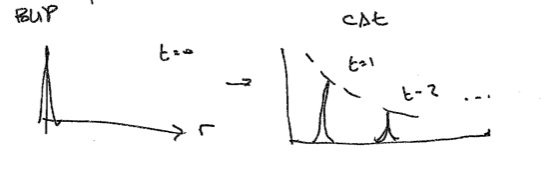
\includegraphics[width=.9\textwidth]{figures/Lec27_3dblip.png}
\end{center}

With a little bit of thought\footnote{This addresses the point in Exercise~\ref{ex:guess:Greens}.}, you could have \emph{guessed} down this Green's function for the wave equation based on the Green's function from the Poisson equation. All you have to do is to remember that the speed of light is constant and you probably want to mathematically enforce causality. In this way, the Poisson equation, the harmonic oscillator, and the wave equation are all \emph{the same damn thing}. They're the appropriate second derivative in a given (3+0)-, (0+1)-, and (3+1)-dimensional spacetime.

To pontificate further on this: all of the uglier versions of the Poisson equation and the wave equation in cylindrical and spherical coordinates are just cousins of what we've done here. Sure, you may have to replace your Fourier expansion over nice plane waves with spherical harmonics or Bessel functions. But you know the deal: we never cared much about the basis functions, we just cared about using the \emph{orthonormality} of these \emph{nice} basis functions to read off the coefficients ($\tilde G$) so that it's easy to represent the solution. Keep this in mind and you won't get lost when you get to the mathematically more tedious examples in your electrodynamics course---you're doing nothing more and nothing less than the harmonic oscillator in some number of dimensions and in some choice of basis.

\begin{exercise}
Solve for the Green's function of the wave equation in (2+1)-dimensional spacetime. Notice that the behavior is quite different from the one in (3+1)-dimensions. Comment on the physics of waves in \emph{Flatland}.
\emph{Answer}:
\begin{center}
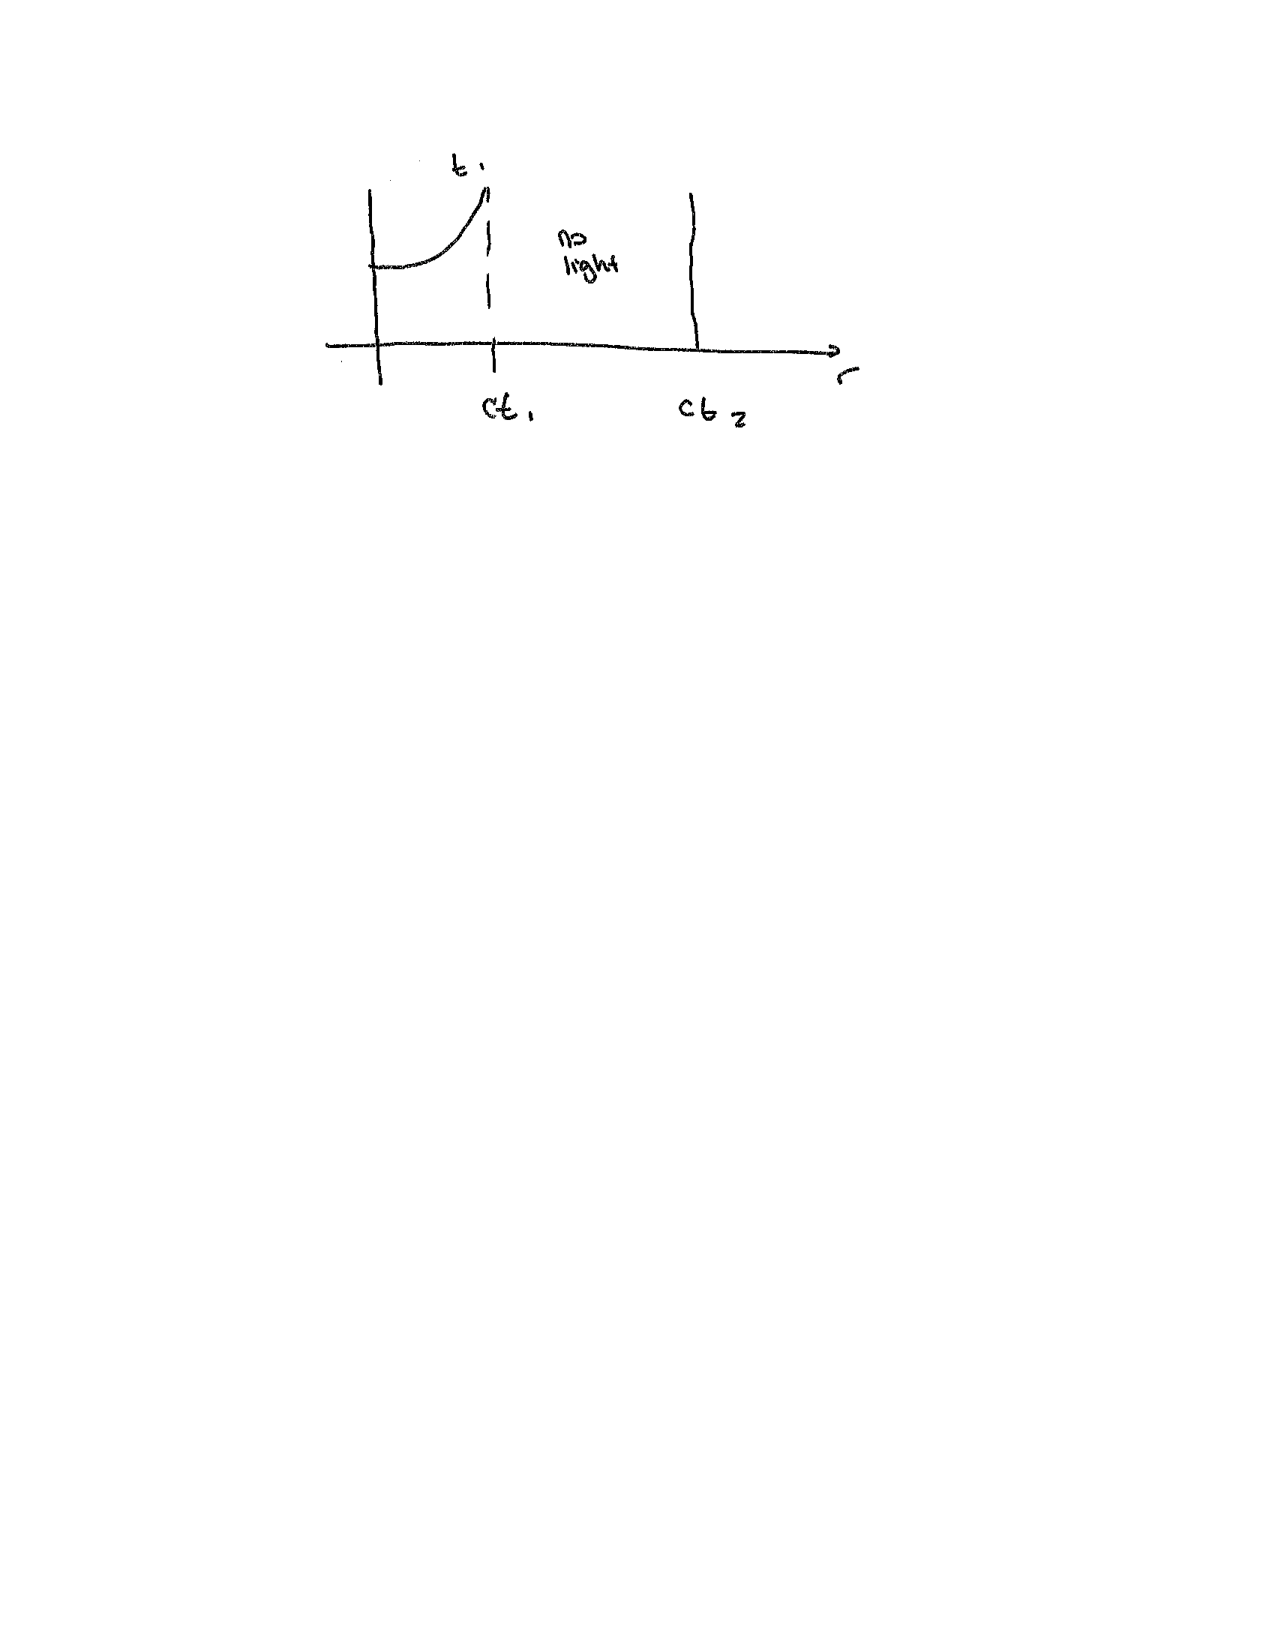
\includegraphics[width=.47\textwidth]{figures/Lec27_2da}
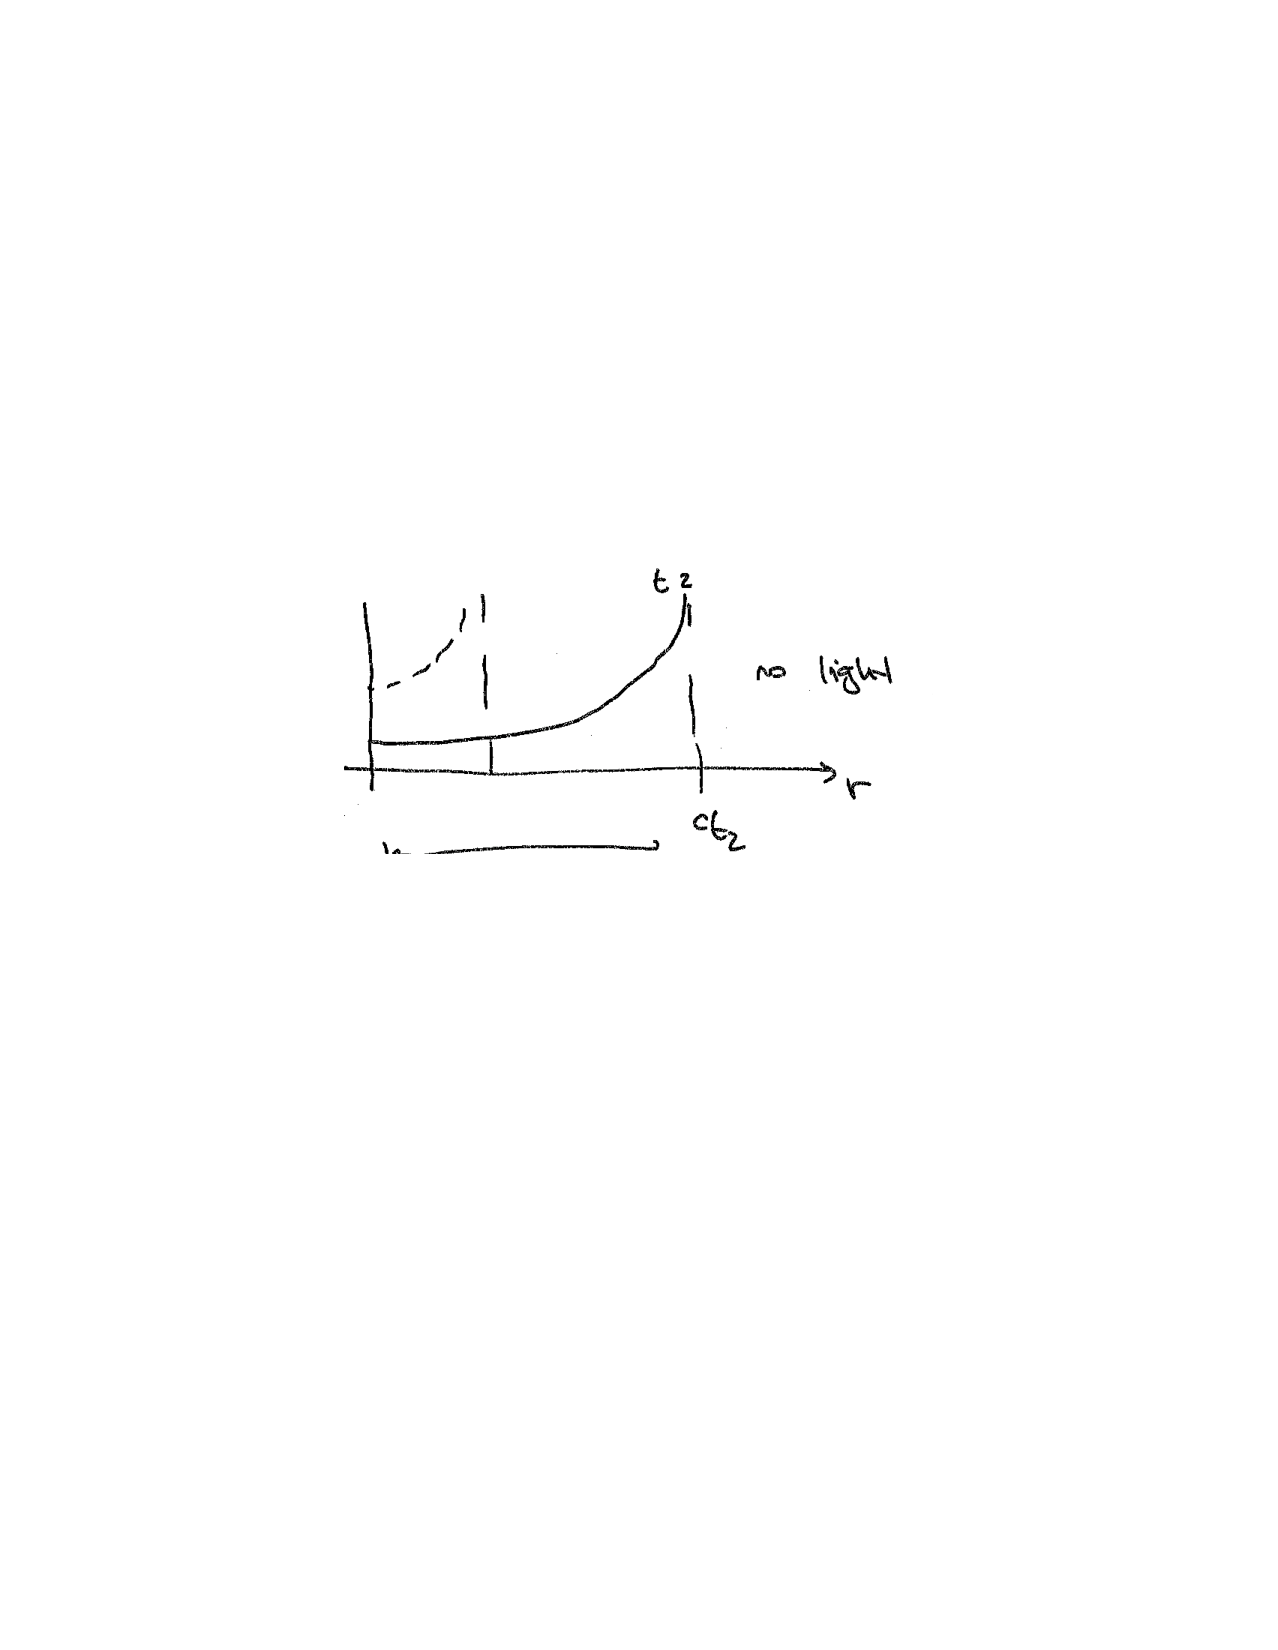
\includegraphics[width=.47\textwidth]{figures/Lec27_2db}
\end{center}
\end{exercise}


\subsection{A theoretical digression}

If you'll permit one further digression, let me remind you that the reason why we spend so much time solving for the second derivative is that our models of physics tend to be local. Consider the action, $S = \int dt \, L$. If we have some state $q$ that propagates in spacetime, the natural form of the action is actually an integral with respect to a Lagrangian \emph{density},
\begin{align}
	S = \int d^4x \mathcal L = \int d^4x \left(\text{const.} + q + \partial_\mu q + \cdots\right) \ ,
\end{align}
where on the right-hand side we just started writing out all possible polynomials of $q(x,t)$ and the four-derivative $\partial_\mu$. If you have been paying close attention, you'll notice that by writing $q(x,t)$ I have surreptitiously passed from $q$ being a `particle' to being a `field'. We only use $\partial_\mu$ instead of $d/dt$ or $\nabla$ because we expect the theory to be Lorentz invariant\footnote{If your theory is not Lorentz invariant, then replace `Lorentz' with whatever symmetries your system does have. If it has no appreciable symmetries, then may Boltzmann have mercy on your soul.}. In fact, we probably don't want to have any terms that have any free indices like $\partial_\mu q$ because that means it transforms like a Lorentz vector and thus the term is not Lorentz invariant. Furthermore, we can use field redefinitions to remove linear terms\footnote{This is not an obvious statement in the action, but the variation of the action usually comes from a path integral, where on varies over $q(x,t)$. Shifting $q(x,t)$ is like integrating $dx$ versus $d(x+3) = dx$.}. Subject to symmetries, the action looks like:
\begin{align}
S = \int d^4x \left[\frac{1}{2}q\left(\partial^2 + \omega_0^2\right)q + cq^3 + dq^4 + e\partial^2 q^2 + \cdots \right]	 \ .
\end{align}
You may recognize that the term in parenthesis is simply the `harmonic oscillator' (or wave equation, they're all the same to me) operator, $\mathcal O$. Indeed, when you vary that part of action by itself, you end up with the appropriate differential equation, $\mathcal O q = 0$. 

What about the other terms? First we should do a bit of dimensional analysis. For my own sanity, let's use natural units where we set $c=\hbar =1$ and all units are measure in mass dimension:
\begin{align}
	[x] = [t] &= -1 \ .
\end{align}
This means that $[d^4x] = -4$. Since the action is dimensionless in natural units---after all, it shows up in a $e^{iS}$---then we know the Lagrangian density has dimension $[\mathcal L] = +4$. Since $[\partial]=+1$, we deduce that the variable $q$ has mass dimension $[q]=+1$. Ok, with that in mind, we can look at the `higher order' terms. The coefficients of these terms must have some \emph{negative} mass dimension:
\begin{align}
	c\, , d\, e \, , \cdots = \left(\frac{1}{M}\right)^n \ ,
\end{align}
where $n$ is a positive integer. We've written the mass scale as $M$. Any mass scale in the theory must have physical significance. We could question whether the mass scale $M$ is big or small compared to either $\omega_0$ or the characteristic energies at which we are studying the system. If $M$ is small, then these coefficients are large, and their dynamics are important. However, if we include these terms in our dynamics, then the equations of motion become very nonlinear:
\begin{align}
	\mathcal O q + 3cq^2 + 4d q^3 + \cdots = 0 \ .
\end{align}
That would mean that the wave equation approximation is quite bad. By the way, those terms are also clearly non-linear. If we see physics that is approximately described by the wave equation, then these coefficients must be small. We thus expect $M$ to be large---it is an ultraviolet scale. 

What we intuit is that the scale $M$ is some energy scale where our theory is breaking down. If, for example, we were to \emph{experimentally}\footnote{In the \emph{gedanken} sense.} study this system at energies $E\sim M$, we expect that the effect of these non-linear terms are no longer small and become significant. In other words, the scale $M$ plays the role of a \emph{cutoff} at which our theory described by the linear operator $\mathcal O$ breaks down. For energies well below $M$, we can study the linear system and do \emph{perturbation theory} to study the first few non-linear coefficients that have coefficients that go like $(1/M)$ to a relatively small power. In the regime where our experiment has characteristic energy $E\ll M$, the in-principle infinite number of higher-order coefficients are negligible because we expect those effects to go like $(E/M)^n$; so keeping the first few should be an accurate description of the system.

This is the notion of an \textbf{effective theory}. All physical models are effective theories. We're simply parameterizing our ignorance about the universe and working in a regime where we are predictive. The effective theory philosophy explains why we are so obsessed with Green's functions of second-derivative operators:
\begin{itemize}
	\item Constant operators are trivial, they're not even differential.
	\item Operators with a single derivative are not Lorentz invariant. (The exceptions, like the diffusion operator, are only valid in the non-relativistic regime.)
	\item Operators with three, five, or any odd number of derivatives are not Lorentz invariant. They are also suppressed by inverse powers of the cutoff, $M$.
	\item Operators that are nonlinear, i.e.~terms in the Lagrangian density that have more than four powers of $q(x,t)$, are also suppressed by inverse powers of the cutoff $M$.
\end{itemize}
This tells you that in (3+1)-dimensions, the most interesting non-linear terms are $\mathcal L \supset cq^3+ dq^4$. If you assume that your theory has some $q\to -q$ symmetry, then you can even remove the $c$ term. By the way, this is how you build theories: you start with the most general $\mathcal L$ with an infinite number of terms. Then you argue based on symmetries and the relevance of high-dimensional operators which terms you can throw out. The result is that any reasonable theory in (3+1)-dimensions should be some perturbation of the harmonic oscillator/wave/Poisson system.

Let me layer onto this a bit more: implicit in writing out $S=\int d^4x\mathcal L$ is the idea that our theory should be manifestly \emph{local}. When we write terms like $q^3$, we really mean $q(x,t)q(x,t)q(x,t)$ at the \emph{same} spacetime point. If this were not true, then the theory would be non-local and the causal structure of the theory would depend on the reference frame. This, in turn would put causality and Lorentz invariance at odds with one another and you'd have to pick one but not both. Some recent alternative formulation of quantum physics based on amplitudes (and not Lagrangians) have proposed that by giving up on \emph{manifest} locality, there may be more elegant descriptions of a theory. Those descriptions are local, they're just not obviously so.

\begin{exercise}
If we lived in Flatland, then the action would take the form $S = \int d^3x \mathcal L$. How does the power counting change for a state $q$? How does it change for a general number of spatial dimensions, $D$? Note: quantum effects can change the story quite a bit in $D=1$ and $D>3$. That's different story
\end{exercise}

\begin{exercise}
The Lagrangian density for electrodynamics is
\begin{align}
	\mathcal L = \frac{1}{4}F^{\mu\nu}F_{\mu\nu} \ ,
\end{align}
where $F_{\mu\nu}$ is the field strength tensor. Write out the corresponding equations of motion. Notice that you only get half of Maxwell's equations. Where does the other half come from? \textsc{Answer} (partial): the other half of Maxwell's equations come from the geometry of that system. It's most clear in the language of differential forms, but then one has to build up that mathematical machinery.
\end{exercise}


% potential future topic: fields from springs













%!TEX root = P231_notes.tex
\section{Coupled Harmonic Oscillators and Fields}
\label{sec:CHO:fields}

Let's take a break from Green's functions. In the previous section, we called the wave equation the \emph{harmonic oscillator in spacetime}. We proceeded to solve the wave equation for the electromagnetic field, $\partial^2 A_\mu = j_\mu$. We were very hand-wavy in arguing that the appropriate generalization of the harmonic oscillator operator $(d/dt)^2$ is the spacetime second derivative, $\partial^2 = c^{-2}\partial_t^2 - \nabla^2$. Furthermore, we noticed that our state functions went from being functions of only one variable, $\psi(t)$, to functions of space and time, $A_\mu(\vec{x},t)$. In other words, our states became \emph{fields}. It's instructive to see why a field is naturally understood as the continuum limit of a lattice of harmonic oscillators\footnote{I'm saying something `deep' here. Actual systems in condensed matter physics are atomic lattices with complicated electronic potentials. These are approximated by harmonic oscillators to leading order. At long wavelengths, the physics of this lattice often has a \emph{continuum limit} described by a field theory. The field theory is a model that has no underlying lattice, but whose long-wavelength predictions are designed to match that of a lattice with small spacing. In particle physics one usually assumes that nature is continuous so that the fundamental objects are actually fields. Whether or not this is literally true doesn't matter: it is sufficient that the range of phenomena that your theory hopes to describe are agnostic to whether or not there is a lattice. Sometimes particle physicists go the opposite way and use lattice techniques to make predictions where the continuum limit is difficult. The notion (and meaning) of a continuum limit is tied closely to the idea or renormalization group flow, which is one of the most elegant ideas in theoretical physics.}.


\subsection{A notational interlude}

Here's a bad habit: I often use the shorthand $x(t)$ to describe the position of a particle at time $t$. The particle doesn't need to literally be a particle, it could be the displacement of a spring from equilibrium. If the particle takes a position in three-space then we write $\vec{x}(t)$. Note that this is very different from a \emph{field}, where the spatial coordinates are a \emph{dependent} variable analogous to time. Just as $x(t)$ has a value for all $t$, a field $\varphi(x,t)$ takes some value for all $x$ and $t$. 

This is a potential source of confusion because we want to show the transition from a single harmonic oscillator to a field. The intermediate state is a lattice of coupled harmonic oscillators. To do this, let us break the bad habit of writing $x(t)$ and write the displacement of a harmonic oscillator to be $q(t)$. The displacement can be abstract, it doesn't have to be a distance separation; for example, it could be the value of a wavefunction at a point in space. If we have a bunch of harmonic oscillators evenly spaced on a line, we can index them $q_i(t)$. 

If you imagine that you have \emph{many} harmonic oscillators that are spaced very closely together, then rather then specifying an index you could just specify their position along the line, $x$. Note that $x$ is playing the role of an index, not as the state variable. In other words:
\begin{align}
	q_i(t) \to q(x,t) \ .
\end{align}
If I pick some point along the line, $x$, then the displacement of the harmonic oscillator at $x$ observed at time $t$ is $q(x,t)$. Congrats, $q(x,t)$ is now a field. You can see why we didn't want to use $x(t)$: it confuses the position along the line with the displacement of the harmonic oscillator at that position. 
%
The picture is as follows:
\begin{center}
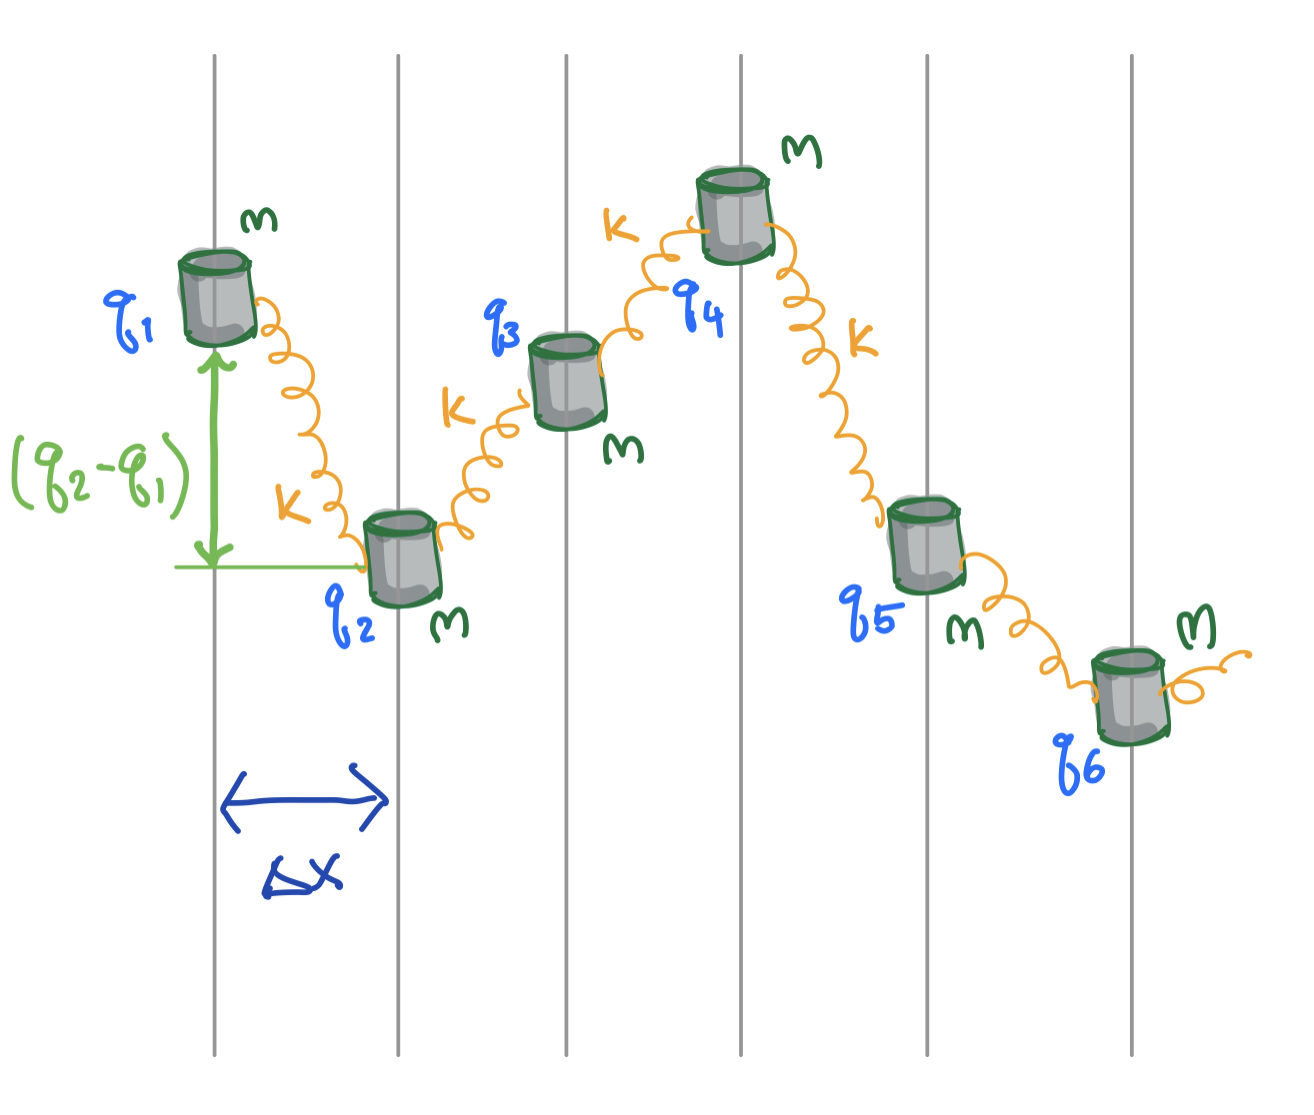
\includegraphics[width=.5\textwidth]{figures/coupledHO.jpg}
\end{center}
The generalization to a dense three-dimensional lattice is straightforward, you end up with $q(x,y,z,t)$ or $q(\vec{x},t)$.


\subsection{Coupled Harmonic Oscillators}
\label{sec:CHO}

The Lagrangian for a single harmonic oscillator $q(t)$ is
\begin{align}
	L[q(t)] &= \frac{1}{2}m \dot q^2 - \frac{1}{2}k q^2 \ .
\end{align}
This assumes some reference equilibrium value $q=0$. Consider instead a series of identical beads of mass $m$ along a line that can move up and down freely, but are connected to their nearest neighbors by springs of uniform spring constant $k$. The Lagrangian for this system is
\begin{align}
	L[q_1(t), q_2(t), \cdots]
	&= 
	\sum_i \frac{1}{2} m \dot q_i^2 
	- 
	\sum_i \frac{1}{2}k (q_i - q_{i-1})^2 \ .
\end{align}
Because life is short, I'm not going to worry about the boundary conditions for the index $i$. You can assume that the system is periodic if you're nervous. Now let us pass into the continuum limit and consider some small separation $\Delta x$. We make the following replacement to continuum variables:
\begin{align}
	i & \rightarrow x
	\\
	q_i(t) & \rightarrow q(x,t)
	\\
	(q_i-q_{i-1})^2 &\rightarrow \Delta x^2 \left(\frac{\partial q}{\partial x}\right)^2
	\\
	\sum_i	&\rightarrow \int \frac{dx}{\Delta x}
	\\
	m &\rightarrow \rho \Delta x \ .
\end{align}
The factors of $\Delta x$ should be clear from dimensional analysis. You can think about them as some characteristic small length scale analogous to the lattice spacing. Observe that the mass of a single harmonic oscillator is replaced by the mass density $\rho$ multiplied by a `volume' ($\Delta x$ in one dimension). Once we write out the Lagrangian the $\Delta x$ factors almost cancel:
\begin{align}
	L 
	&= \int \frac{dx}{\Delta x} \, 
	\left[
		\frac{1}{2}\rho \Delta x 
		\left(\frac{\partial q}{\partial t}\right)^2 
		- 
		\frac{1}{2}k \Delta x^2
		\left(\frac{\partial q}{\partial x}\right)^2
	\right]
	\\
	&= \int dx\,
	\left[
		\frac{1}{2}\rho 
		\left(\frac{\partial q}{\partial t}\right)^2 
		- 
		\frac{1}{2} \left(k \Delta x\right)
		\left(\frac{\partial q}{\partial x}\right)^2
	\right] \ .
\end{align}
If we had a lattice in $D$ spatial dimensions, then this result generalizes to
\begin{align}
	L 
	&= \int d^Dx\,
	\left[
		\frac{1}{2}\rho 
		\left( \frac{\partial q}{\partial t} \right)^2 
		- 
		\frac{1}{2} \left(k \Delta x^{2-D}\right)
		\left(\frac{\partial q}{\partial \vec{x}}\right)^2
	\right] \ .
	\label{eq:HO:coupled:D}
\end{align}
Finally, let us rescale the state variable by defining a `better' state variable
\begin{align}
	\varphi(x,t) \equiv \frac{q(x,t)}{\sqrt{\rho}} \ .
\end{align}
Further, let's go ahead and write the action $S=\int dt \, L$ with the idea of writing one big \emph{spacetime} integral over a Lagrangian \emph{denstiy} $S = \int dt\, d^Dx \, \mathcal L$:
\begin{align}
	S = \int dt \, d^Dx \,
	\frac{1}{2}
	\left[
	\left( 
		\frac{\partial \varphi}{\partial t}
		\right)^2
	- 
	c^2
	\left(\frac{\partial \varphi}{\partial \vec{x} }\right)^2
	\right] \ .
\end{align}
Observe that we have defined a speed
\begin{align}
	c^2 = k \Delta x^{2-D} \rho \ .
	\label{eq:HO:coupled:D:c2}
\end{align}
If we take one more step and integrate by parts, we may write the action in the form:
\begin{align}
	S = \int dt \, d^Dx \,
	\frac{-c^2}{2}
	\varphi
	\left[
	\frac{1}{c^2}
	\left( 
		\frac{\partial}{\partial t}
		\right)^2
	- 
	\left(\frac{\partial }{\partial \vec{x} }\right)^2
	\right]
	\varphi 
	&=
	-c^2 \int d^{D+1}x \frac{1}{2} \varphi \partial^2 \varphi 
	\ .
\end{align}
Aha! Check it out, we have recovered the \emph{wave operator} $\partial^2$.  Now if you permit me some sloppy calculus, then if I squint at the action $S$ and vary with respect to $\varphi$, I get 
\begin{align}
	\delta S &=0 
	&\Rightarrow&&
	\partial^2 \varphi &= 0 \ .
\end{align}
Let's be completely honest: we should do this variation more carefully... and we will, but just not right now. But this result is rather compelling: $\partial^2\varphi(x,t) = 0$ is simply the wave equation.
\begin{exercise}
Confirm that \eqref{eq:HO:coupled:D} is the appropriate generalization to $D$ spatial dimensions.
\end{exercise}
\begin{exercise}
Confirm by dimensional analysis that $c$ in \eqref{eq:HO:coupled:D:c2} is a speed.
\end{exercise}

\subsection{Interpretation}

What we have described here is a lattice of harmonic oscillator states. The harmonic oscillator potential comes from each lattice point being connected `by a spring' to its nearest neighbor lattice points in each spatial direction. The propagation of a wave comes from a perturbation of single harmonic oscillator \emph{locally} affecting the harmonic oscillators nearby. Those oscillators, in turn, cause perturbations to \emph{their} neighbors. The speed $c$ is a characteristic speed of this propagation. In the continuum theory it's just some prefactor that is required by dimensional analysis. In the lattice theory it is related to the mass of each harmonic oscillator and the spring constant. 

Now that we've gone from the lattice to the continuum, you can just look at the Lagrangian for a field and see that it can be understood as each local piece of the field tugging at nearby parts of the field. 

\begin{example}
The relative minus sign between the time derivatives and the space derivatives in $\partial^2 = c^{-2}\partial_t^2 - \nabla^2$ is understood as the relative minus sign between the kinetic term and the potential term in the Lagrangian\footnote{You could, in turn, ask where that relative minus sign comes from. There are a few different ways to answer this, but I think the way that makes the most sense to me the one that is based on the path integral formulation of quantum mechanics.} 
\end{example}

\begin{exercise}
We assumed that each harmonic oscillator in the lattice has an identical mass $m$ and an identical spring constant $k$. What is the physical significance of this choice in the continuum representation?
\end{exercise}

\begin{exercise}
We assumed that each harmonic oscillator on the lattice only couples to its nearest neighbor. What would interactions with next-to nearest neighbors look like in the continuum representation? What is a good physical reason why you wouldn't have couplings to lattice points that are very far away\footnote{You can think about this problem the other way around and consider that the choice of the nearest neighbor couplings is \emph{defining} a sense of spacetime locality. Some theorists thinking about the nature of quantum mechanics propose that an analogous idea with quantum entanglement may be responsible for the macroscopic emergence of spacetime. See, e.g.~\texttt{arXiv:1606.08444}.}? \textsc{Hint}: we've already discussed this when we presented discretized function space... the only difference was when we did that, we started with a continuum and motivated a discrete representation. Now we're going in the other direction.
\end{exercise}


\subsection{A theoretical digression}
\label{sec:EFT:philosophy}

If you'll permit yet another digression, let me remind you that the reason why we spend so much time solving for the second derivative is that our models of physics tend to be local. Consider the action, $S = \int dt \, L$. If we have some state $\varphi$ that propagates in spacetime, then $\varphi$ is a \emph{field}. The natural form of the action is an integral with respect to a Lagrangian \emph{density},
\begin{align}
	S = \int d^4x \mathcal L = \int d^4x \left(\text{const.} + a \varphi + b \partial_\mu \varphi + \cdots\right) \ ,
\end{align}
where on the right-hand side we just started writing out \emph{all} possible polynomials of $\varphi(x,t)$ and the four-derivative $\partial_\mu$ with respect to coefficients $a, b,\cdots$. At this point we're not writing \emph{the} theory of the field $\varphi$, we are parameterizing \emph{all} theories of the field $\varphi$. Different choices for the infinite number of coefficients (typically called \emph{couplings}) correspond to different theories of the field $\varphi$.

We have already seen that the wave operator $\partial^2$ emerges from the kinetic term and the nearest-neighbor harmonic oscillator coupling on a lattice of spatial points. As we imagine the infinite sum of all possible terms in the action $S$, we write $\partial_\mu$ instead of $d/dt$ or $\nabla$ because we expect the theory to be Lorentz invariant\footnote{If your theory is not Lorentz invariant, then replace `Lorentz' with whatever symmetries your system does have. If it has no appreciable symmetries, then may Boltzmann have mercy on your soul.}.  In fact, we probably don't want to have any terms that have any free indices like $\partial_\mu \varphi$ because that means it transforms like a Lorentz vector and thus the term is not Lorentz invariant. Furthermore, we can use field redefinitions to remove linear terms\footnote{This is not an obvious statement in the action, but the variation of the action usually comes from a path integral, where on varies over $\varphi(x,t)$. Shifting $\varphi(x,t)$ is like integrating $dx$ versus $d(x+3) = dx$.}. Subject to symmetries, the action looks like:
\begin{align}
S = \int d^4x \left[\frac{1}{2}
%q\left(\partial^2 + \omega_0^2\right)q 
\left(\partial \varphi\right)^2
- \frac{1}{2}\omega_0^2 \varphi^2
+ c\varphi^3 + d\varphi^4 + e\partial^2 \varphi^2 + \cdots \right]	 \ .
\end{align}
You recognize that the term in parenthesis is simply the wave operator. It is usually convenient to lump together all of the quadratic terms
\begin{align}
	S_\text{quad.} 
	= 
	\int d^4x \, \left(\partial \varphi\right)^2
	- \frac{1}{2}\omega_0^2 \varphi^2
	=
	-
	\frac{1}{2}
	\int d^4x \, \varphi \,\mathcal{O}_\text{quad}\,\varphi \ .
\end{align}
When you vary this part of action and ignore the other terms, you end up with the appropriate \emph{linear} differential equation, $\mathcal O \varphi = 0$. This should make sense from basic calculus: if you have a quadratic function $f(x)=\frac{1}{2}ax^2$, then the first derivative is linear: $f'(x)=ax$ and the extrema satisfy $ax=0$. The wave equation comes from the same observation when you replace $x\to \varphi$ and $a\to \mathcal O_\text{quad.}$. Of course you're really going from a function $f(x)$ to a functional (function of functions) $S[\varphi]$, but this is a technical detail\footnote{You may want to check that this intuition is true by again imagining a discretized version of $\varphi$.}.


The operator $\mathcal{O}_\text{quad}$ includes the usual wave equation that represented a lattice of coupled harmonic oscillators, as well as the term $\omega_0^2 \varphi(x)^2$.  
\begin{exercise}
The $\omega_0^2$ term looks like the potential for a harmonic oscillator. How is it different from the $\nabla^2$ harmonic oscillator potential? How would you describe a lattice of harmonic oscillators with both the $\nabla^2$ and the $\omega_0^2$ potentials? \textsc{Hint}: what is the equilibrium value of the harmonic oscillators?
\end{exercise}

What about the other terms? First we should do a bit of dimensional analysis. For my own sanity, let's use natural units where we set $c=\hbar =1$ and all units are measure in mass dimension:
\begin{align}
	[x] = [t] &= -1 \ .
\end{align}
This means that $[d^4x] = -4$. Since the action is dimensionless in natural units---after all, it shows up in a $e^{iS}$---then we know the Lagrangian density has dimension $[\mathcal L] = +4$. Since $[\partial]=+1$, we deduce that the variable $q$ has mass dimension $[\varphi]=+1$. With that in mind, we can look at the `higher order' terms. The coefficients of these terms must have some \emph{negative} mass dimension:
\begin{align}
	c\, , d\, , e \, , \cdots = \left(\frac{1}{M}\right)^n \ ,
\end{align}
where $n$ is a positive integer. We've written the mass scale as $M$. Any mass scale in the theory must have physical significance. We could question whether the mass scale $M$ is big or small compared to either $\omega_0$ or the characteristic energies at which we are studying the system. If $M$ is small, then these coefficients are large, and their dynamics are important. However, if we include these terms in our dynamics, then the equations of motion become very nonlinear:
\begin{align}
	\mathcal O_\text{quad.} q + 3c\varphi^2 + 4d \varphi^3 + \cdots = 0 \ .
\end{align}
That would mean that the wave equation approximation is quite bad. Further, these additional terms are also clearly non-linear.  If we see physics that is approximately described by the wave equation, then these coefficients must be small. We thus expect $M$ to be large---it is an ultraviolet scale. 

What we intuit is that the scale $M$ is some energy scale where our theory is breaking down. If, for example, we were to \emph{experimentally}\footnote{In the \emph{gedanken} sense.} study this system at energies $E\sim M$, we expect that the effect of these non-linear terms are no longer small and become significant. In other words, the scale $M$ plays the role of a \emph{cutoff} at which our theory described by the linear operator $\mathcal O_\text{quad.}$ breaks down. For energies well below $M$, we can study the linear system and do \emph{perturbation theory} to study the first few non-linear coefficients that have coefficients that go like $(1/M)$ to a relatively small power. In the regime where our experiment has characteristic energy $E\ll M$, the in-principle infinite number of higher-order coefficients are negligible because we expect those effects to go like $(E/M)^n$; so keeping the first few should be an accurate description of the system.

This is the notion of an \textbf{effective theory}. All physical models are effective theories. We're simply parameterizing our ignorance about the universe and working in a regime where we are predictive. The effective theory philosophy explains why we are so obsessed with Green's functions of second-derivative operators:
\begin{itemize}
	\item Constant operators are trivial, they're not even differential.
	\item Operators with a single derivative are not Lorentz invariant. (The exceptions, like the diffusion operator, are only valid in the non-relativistic regime.)
	\item Operators with three, five, or any odd number of derivatives are not Lorentz invariant. They are also suppressed by inverse powers of the cutoff, $M$.
	\item Operators that are nonlinear, i.e.~terms in the Lagrangian density that have more than four powers of $q(x,t)$, are also suppressed by inverse powers of the cutoff $M$.
\end{itemize}
This tells you that in (3+1)-dimensions, the most interesting non-linear terms are $\mathcal L \supset c\varphi^3+ d\varphi^4$. If you assume that your theory has some $q\to -q$ symmetry, then you can even remove the $c$ term. By the way, this is how you build theories: you start with the most general $\mathcal L$ with an infinite number of terms. Then you argue based on symmetries and the relevance of high-dimensional operators which terms you can throw out. The result is that any reasonable theory in (3+1)-dimensions should be some perturbation of the harmonic oscillator/wave/Poisson system.

Let me layer onto this a bit more: implicit in writing out $S=\int d^4x\mathcal L$ is the idea that our theory should be manifestly \emph{local}. When we write terms like $q^3$, we really mean $\varphi(x,t)\varphi(x,t)\varphi(x,t)$ at the \emph{same} spacetime point. If this were not true, then the theory would be non-local and the causal structure of the theory would depend on the reference frame. This, in turn would put causality and Lorentz invariance at odds with one another and you'd have to pick one but not both. Some recent alternative formulation of quantum physics based on amplitudes (and not Lagrangians) have proposed that by giving up on \emph{manifest} locality, there may be more elegant descriptions of a theory. Those descriptions are local, they're just not obviously so.

\begin{exercise}
If we lived in Flatland, then the action would take the form $S = \int d^3x \mathcal L$. How does the power counting change for a state $q$? How does it change for a general number of spatial dimensions, $D$? Note: quantum effects can change the story quite a bit in $D=1$ and $D>3$. That's different story
\end{exercise}

\begin{exercise}
The Lagrangian density for electrodynamics is
\begin{align}
	\mathcal L = \frac{1}{4}F^{\mu\nu}F_{\mu\nu} \ ,
\end{align}
where $F_{\mu\nu}$ is the field strength tensor. Write out the corresponding equations of motion. Notice that you only get half of Maxwell's equations. Where does the other half come from? \textsc{Answer} (partial): the other half of Maxwell's equations come from the geometry of that system. It's most clear in the language of differential forms, but then one has to build up that mathematical machinery.
\end{exercise}

Finally, let me end this theoretical digression by re-emphasizing the effective theory philosophy. For the most part, a theory for the field $\varphi$ is an action with respect to this field. The equation of motion for the field come from $\delta S = 0$. The quadratic terms in $\varphi$ give a linear differential equation $\mathcal O_\text{quad} \varphi = 0$. In the presence of a source\footnote{One way to write the source is to put in a linear term in the Lagrangian density with the source $j(x)$ as a coefficient, $\Delta\mathcal L = -j(x)\varphi(x)$. The resulting differential equation is $\mathcal O_\text{quad.}\varphi =j(x)$.} there's some non-trivial right-hand side. This linear equation can be solved using Green's functions. The terms coming from higher powers of $\varphi$ are \emph{non-linear}, but they are also small as long as the theory is being studied at energies that are small compared to the dimensionful scale $M$ that suppresses those terms. This is the regime where the theory is under control (perturbative) and where it makes sense to talk about excitations of the $\varphi$ field. At much higher energies, this description may break down---for example, because it may become important to include the infinite number of non-linear terms. Or perhaps the underlying theory is a completely different theory where $\varphi$ were effective degrees of freedom.
\begin{example}
Our theories of protons, neutrons, and electrons make sense until you study them at energies $E>\text{GeV}$ at which point the substructure of the nucleons becomes important. The protons and neutrons are no longer fundamental degrees of freedom and are replaced by a new description, quantum chromodynamics, that looks nothing like a theory of protons and neutrons. To say it differently, a chef doesn't need to know plasma physics when boiling a soup at 373 Kelvin. However, if you want to describe the phase transitions of early universe at $10^{13}$ Kelvin, then you really do need to know about subnuclear physics. The \emph{relevant} description of nature depends on the energy scale. Often times, the idea of a \emph{relevant} description is far more important than getting \emph{the right} description\footnote{One of the most intriguing ideas in theoretical physics is the existence of dualities that relate the mathematical description of two completely different theories. One of the implications of these observations is that there may not be a single `right' description of nature at a given energy scale. It may be that many completely different-looking theories make equivalent predictions about the same phenomena. Typically, though, only one of these descriptions is perturbative and easily calculable. Turning this observation upside down, one may use these dualities as a way to understand what happens to one description of nature when it breaks down---perhaps a dual description that was non-perturbative becomes perturbative in that break-down region. This turns out to be one of the main motivations to study extra dimensions.}.
\end{example}

If we only took the quadratic part of the action, then the theory is completely linear and every field looks like it's described by the wave equation. We call that case a \emph{free} field theory because it has no interactions and is completely solvable. Theories are distinguished by the kinds of interactions that \emph{perturb} the linear theory. Suppose, for example, we included a $-\lambda \varphi^4$ term in the action. Now we have a theory that is not \emph{just} the wave equation---in fact, it is not even linear. Since our theory is non-linear, what good is any of the Green's function garbage we've learned in this class?! There are two standard options:
\begin{itemize}
	\item Numerical approach: simulate the system on a lattice and solve for the extrema of the action. This is called lattice QCD in the high-energy physics community. In the astronomy community this is just called `simulation.' 
	\item Feynman diagrams: do perturbation theory with respect to the couplings as long as they are small. 
\end{itemize}
I have little to say about the numerical approach other than that it is limited by computing power. There's always a handful of open questions in physics that one wonders: if we focused all of our supercomputing power on this problem for a week, maybe humanity would just know the answer.

The Feynman diagram approach is limited by perturbativity. The idea, though, is that you can use the Green's function from the linear (quadratic) part of the theory, but you have to \emph{perturb} about this Green's function by inserting powers of the non-linearity. The Green's function encodes the propagation of information from a source point in spacetime to the observation point in spacetime, hence the alternative name of `propagator'. When you include the non-linearities, you systematically deform the Green's function at intermediate points in spacetime. This is most easily represented graphically by diagrams where straight lines represent linear propagation through spacetime and vertices represent non-linear perturbations. For example, the $\varphi^4$ term is a vertex connecting four lines: this is because it's like four `harmonic oscillators' that are chained together; when one of them wiggles (because a wave hits it), it causes the other three to wiggle and leads to \emph{three} outgoing waves. We leave a careful exploration of this technique to a course on statistical field theory or quantum field theory. 

\begin{example}
If you have two fields, $\varphi$ and $\psi$, then the effective theory approach follows. You imagine writing down not only all possible polynomials in each field alone, but mixed polynomials like $\varphi^2\psi^2$ subject to the symmetries of your theory. The more symmetric your theory, the fewer terms are allowed. Higher-order terms that are suppressed by large powers of the heavy scale $M$ are negligible compared to terms with smaller $M$-suppression.
\end{example}


% potential future topic: fields from springs













%!TEX root = P231_notes.tex
\section{Green's Functions, Statistics, and Gaussian Integrals}

In Section~\ref{sec:CHO:fields} we showed how fields emerge from a system of nearest-neighbor coupled harmonic oscillators. To leading order, fields are described by the wave operator. We remarked that the differential equation that governs a physical theory comes from a variation of the action functional $\delta S[\varphi]=0$. We even motivated how one builds theories: you start by imagining the most general action $S$ and then you remove terms because they violate symmetries or because they're suppressed by an energy scale $M$ much larger than the energy $E$ or physical phenomena you're examining. The latter point amounts to a $(E/M)^n$ suppression on physical observables. 

At this point, you may ask: well, where does $\delta S = 0$ come from? Curious, aren't we? It turns out that this connects to a few different ideas which we'll map out in this section. In case you haven't noticed, the latter part of these notes are much less technical than the first half. The point is no longer to teach you techniques. We are stepping back and seeing how these ideas interconnect with different theoretical structure that you may [soon] know. Don't worry if there are more results that are left to you to prove or look up, the goal isn't the technical derivation. The goal is to see the interconnection of these tools.

In this section, we'll make a connection to a bit of probability theory and a cute trick for solving Gaussian integrals. First, though, a quantum mechanical interlude.

\subsection{Quantum Mechanics: Green's Function from the Path Integral}

Time evolution by some amount of time $\Delta t$ in quantum mechanics is enacted by the Hamiltonian (energy) as an operator: $e^{i\hat H\Delta t}$. This time evolution may be described as a Green's function that takes an initial state $\Psi(q_0,t_0)$ and evolves it into a final state $\Psi(q, t)$. The wavefunctions are defined by a projection of a state $|\psi(t)\rangle$ onto the position basis $q$:
\begin{align}
	\Psi(q,t) = \langle q | \psi(t) \rangle \ .
\end{align}
Since $|\psi(t)\rangle$ is the time evolution of $|\psi(t_0)\rangle$ by a time $\Delta t = t-t_0$, we may continue:
\begin{align}
	\Psi(q,t) 
	&= \langle q | e^{-i\hat H \Delta t} |\psi(t_0) \rangle
	\\
	&= \int dq_0\langle q | e^{-i\hat H \Delta t} |q_0 \rangle\langle q_0 |\psi(t_0) \rangle 
	\\
	&= \int dq_0\,\langle q | e^{-i\hat H \Delta t} |q_0 \rangle \Psi(q_0, t_0)
	\ ,
\end{align}
where we have simply inserted a complete set of states (\emph{multiplied by one}) $\mathbbm{1} = \int dq_0 |q_0 \rangle\langle q_0 |$; this is simply the completeness relation that we recall from our review of linear algebra. We identify the quantity $\langle q | e^{-i\hat H \Delta t} |q_0 \rangle$ as the Green's function $G(q,t;q_0,t_0)$ since it now manifestly plays the role of a Green's function to solve for the state $\Psi(q,t)$ given the initial state $\Psi(q_0, t_0)$:
\begin{align}
	\Psi(q,t)\, 
	&= \int dq_0\, G(q,t;q_0,t_0) \Psi(q_0, t_0)
	\ . 
\end{align}
We didn't have to explicitly write the Schr\"odinger equation because that's already implicit in our starting point that $e^{-i\hat H \Delta t}$ is the time-evolution operator. 

If you go over the path integral formulation of quantum mechanics, one finds that by repeating this trick and inserting a complete set of states over \emph{many} time slices between $t_0$ and $t$ you end up with\footnote{You may refer to the first couple of lectures here: \url{https://sites.google.com/ucr.edu/p230b/}} a closed form expression for the Green's function:
\begin{align}
	G(q,t;q_0,t_0)  = \int \mathcal Dq(t) \, e^{iS[q]/\hbar} \ .
	\label{eq:G:QM}
\end{align}
\begin{exercise}
For those with some familiarity with quantum mechanics, derive the above result. Be sure to keep track of how $e^{i\hat H t}$ turns into $e^{iS[q]}$. I personally find this to be the most compelling motivation for defining the action $S$ as the difference of the kinetic and the potential energies. Hint: you can slice up the finite time interval $t$ into a bunch of tiny time slices $\varepsilon t$. You can use the following matrix/operator relation: $e^{\varepsilon(A+B)} = e^{\varepsilon A}e^{\varepsilon B}+\mathcal O(\varepsilon^2)$ to separate out the kinetic and potential terms. Note that the kinetic terms depend only on momentum while the potential terms depend only on position. You can insert complete sets of momentum states, $\mathbbm 1 = \int dp |p\rangle \langle p|$ (check the normalization) and use $\langle q|p\rangle \sim e^{ipq}$, subject to conventions.
\end{exercise}
I've broken my usual convention of natural units and explicitly written out the $\hbar$ required to make $S[q]$ dimensionless. Recall that $[L]$ is energy and $S = \int dt \, L$ so that $[S] = E\times t$, which just happens to be the units of $\hbar$. The curious integration measure $\mathcal Dq(t)$ is an integral over different functions $q(t)$. The meaning is clear if we discretize in time:
\begin{align}
	\mathcal D q(t) = dq(t_0)\,dq(t_1)\,dq(t_2)\,\cdots dq(t_{N-1})\,dq(t_N = t) \ .
\end{align}
In other words, for each discrete time $t_i$, we vary the position $q(t_i)$ independently of the other positions. In this way, the integral over $\mathcal D q(t)$ is an integral over all possible functions $q(t)$ subject to the initial and final states.

You should interpret this expression as the famous quantum mechanical \emph{sum over histories}. The amplitude for a state to go from $\Psi(q_0,t_0)$ to $\Psi(q,t)$ includes a sum over the amplitude for each possible way to transition from the initial to the final state. At this point, you should recall the double slit experiment\footnote{The argument goes like this: imagine a double slit experiment. Now poke a third slit through the board; you sum over three paths. Now insert another board with two slits; you sum over $3\times 2 = 6$ paths. Now poke more holes, add more boards until you have an infinite number of boards each with an infinite number of holes. This corresponds to summing over all possible continuum paths from the initial to the final positions.}.
%
Evidently the quantity $e^{iS/\hbar}$ is the weight of each path. It corresponds to the amplitude of each path we're summing together. The total amplitude is given by the sum of these complex numbers with unit magnitude\footnote{You may want to look up `phasor' diagrams to see how to interpret this sum. Feynman describes this well in his for-the-public book \emph{QED: The Strange Theory of Light and Matter}, or you can see a more recent pop physics summary from PBS Spacetime: \url{https://youtu.be/vSFRN-ymfgE}.}.

$\hbar$ is also a measure of `quantumness'. Recall that it shows up in statistical mechanics due to the Gibbs paradox. The `quantum' of quantum mechanics refers to the fact that $\hbar\neq 0$ so that $[\hat p, \hat q] \neq 0$. As $\hbar\to 0$ one recovers the classical limit. We see that in the classical limit, the argument of the exponential $e^{iS/\hbar}$ becomes large and highly sensitive to variations of $S$. At this point one can make the \emph{saddle point approximation}. This is the observation that for $\hbar\to 0$, changes in $S[q]$ coming from nearby paths will rapidly change the phase of $e^{iS/\hbar}$ and cause the contributions of these nearby paths to cancel as one integrates over paths $q(t)$. There is one exception: when $S[q]$ is near an extremum (say, a minimum) then the contribution from nearby paths will change more slowly---this is obvious, you're at an extremum so the functional $S[q]$ is flat---and the those paths will dominate the integral. The result is that in the classical limit, the paths $q(t)$ that give the dominant contribution are simply those which realize an extremum of the action:
\begin{align}
	\delta S[q] = 0 \ .
\end{align}
And there you go, we have `derived' the principle of least action as the classical limit of time evolution in quantum mechanics. 

\begin{exercise}
How do you expect the Green's function \eqref{eq:G:QM} to change when we go from a \emph{particle} at $q(t)$ at time $t$ to a \emph{field} $\varphi(x,t)$ that takes in position $x$ and time $t$ as variables?  Congratulations, you're on your way to quantum field theory. 
\end{exercise}

\subsection{A probability refresher}

Now you may have a bit of mental whiplash as I change gears completely, but humor me a moment, we'll get back to the quantum mechanical picture shortly. 

A probability distribution function is an integrand $p(x)dx$ that tells you about the probability for some quantity $x$ to take some value. $p(x)$ is an infinitesimal probability defined by the statement that the probability for $x$ to take values within $x$ and $(x+dx)$ is $p(x)dx$. The probability for $x$ to take a value within some finite range $x\in[a,b]$ is
\begin{align}
	P(x\in[a,b]) = \int_a^b dx\, p(x) \ .
\end{align}
As you can expect, distributions are normalized so that
\begin{align}
	\int_{-\infty}^{\infty} dx\, p(x) = 1 \ .
\end{align}
A surprising amount of physics boils down to probability distributions. This shows up because we often deal with thermal/statistical uncertainty in condensed matter systems, data uncertainty in observational and experimental fields, and quantum uncertainty in anything `small.' Often you get multiple kinds of uncertainty\footnote{There's also the notorious `theory' uncertainty which is a statement about us not knowing what we don't know.}. Physics trains us to be skeptics. This is also part of what makes research-level training in physics so valuable in many other fields like machine learning or finance\footnote{It's almost surprising that this hasn't translated into fields like government and policy, though I suspect that this may be due to aspects that are lacking from a traditional physics training.}.

\begin{example}
The most famous distribution is the Gaussian:
\begin{align}
	g(x) &= \frac{1}{\sqrt{2\pi \sigma^2}} e^{\frac{-(x-\mu)^2}{2\sigma^2}} \ .
\end{align}
This is a distribution with mean $\mu$ and standard deviation $\sigma$. It is relevant for us in this course because up to pre-factors, it is an exponential of a quadratic polynomial---this looks similar to $e^{iS}$, where we argued that the quadratic parts of $S$ correspond to terms that give linear differential equations.
\end{example}

A probability distribution can be decomposed into moments. This the same way that you can decompose a finite mass distribution into \emph{moments} of inertia or the way that we can decompose a charge distribution into monopoles, dipoles, quadrupoles, etc. The $n^\text{th}$ moment of a distribution $p(x)$ is
\begin{align}
	M_n = \int_{-\infty}^\infty dx \, x^n p(x) \equiv \langle x^n \rangle \ .
\end{align}
The notation should remind you of a `correlation function' or an `expectation value.' The moments are an expansion that encode the whole distribution. There is, in turn, a fancy way to encode the moments in a \textbf{generating function}:
\begin{align}
	Z(J) \equiv \int dx\, e^{J x} \, p(x) \  
	= \langle e^{J x}\rangle
	= \langle 1 \rangle + J \langle x\rangle
	+ \frac{1}{2}J^2 \langle x^2\rangle + \cdots \ ,
	\label{eq:generating:function}
\end{align}
where $J$ is the argument of the generating function. The moments of the distribution are derivatives of the generating function:
\begin{align}
	M_n =
	\left.\frac{\partial^n Z(J)}{\partial J^n}\right|_{J = 0} \ .
\end{align}
The generating function is a \emph{Laplace transform} of the distribution $p(x)dx$. Like the Fourier transform, this is an integral transform that can be used to solve differential equations. To the best of my limited experience, engineers learn about Laplace transforms and physicists learn about Fourier transforms\footnote{I suspect this is because the momentum basis has physical significance for us. Maybe engineers are a little more skeptical of imaginary numbers than we are. Who knows. ... okay, I suspect someone with a mathematical background knows and will say that both physicists and engineers are being silly. \url{https://xkcd.com/435/}}.
\begin{example}
One could also write the Fourier transform of the distribution $p(x)dx$. This is called the \textbf{characteristic function} and is defined by
\begin{align}
	\tilde p(k) = \int_{-\infty}^\infty dx\, e^{ikx}p(x) = 1 + ikM_1 + \cdots \ .
\end{align}
\end{example}

\begin{example}
Observe that $\tilde p(k) = Z(ik)$.
\end{example}

\begin{example}
Note that one can write the distribution in a Fourier representation:
\begin{align}
	p(x) &= \int \dbar k 
	\left( 1+ikM_1 + \frac{(ik)^2}{2!}M_2 + \cdots \right)e^{-ikx} \ .
\end{align}
The $e^{-ikx}$ looks like a $\delta$-function in momentum space\footnote{This is a toy version of the partition function in quantum field theory and the $\delta$-function imposes overall momentum conservation on any scattering process.}. In fact, we can think of this as a derivative expansion:
\begin{align}
	p(x) &= \int \dbar k \left( 1+ \left(-\partial_x\right) M_1 + \frac{\left(-\partial_x\right)^2}{2!}M_2 + \cdots \right)e^{-ikx} \ .
\end{align}
Recalling that $\int \dbar k e^{-ikx} = \delta(x)$, we see that this is indeed an expansion in derivatives of the $\delta$-function:
\begin{align}
	p(x) &= \left[ 1+ \left(-\partial_x\right) M_1 + \frac{\left(-\partial_x\right)^2}{2!}M_2 + \cdots \right] \delta(x) \ .
\end{align}
This means that if we would like to determine the expectation value of a test function, $\langle f(x)\rangle$, with respect to the distribution $p(x)$, we have
\begin{align}
	\langle f(x)\rangle = \int dx\, f(x)\, p(x) = f(0) + m_1 f'(0) + \cdots \ .
\end{align}
\end{example}



\subsection{If this were a different class}

If this were a different class, we would take a moment and talk about probabilities in physics. Rather than doing that, let me refer to some fun ideas in Appendix~\ref{sec:probability}.

\subsection{A cute trick: the Gaussian integral}

One of the neat things that you can show off to any young family members is the Gaussian integral. Removing annoying prefactors, one could imagine asking a high school student to integrate the Gaussian:
\begin{align}
	G = \int_{-\infty}^\infty dx\, e^{-\frac{1}{2}x^2} \ .
\end{align}
The exponent is supposed to be easy to solve, but the argument is quadratic. A change of variables doesn't help. What can we do?

It turns out we can simplify the problem by solving it in two dimensions. We may write $G^2$ as a two dimensional integral over independent variables:
\begin{align}
	G^2 = \int dx\, dy\, e^{-\frac{1}{2}(x^2 + y^2)} \ .
\end{align}
The trick is to pass to polar coordinates:
\begin{align}
	G^2 &= 2\pi \int_0^\infty\, r\,dr\, e^{-\frac{1}{2}r^2}
	\\
	&= 2\pi \int_0^\infty\, dw\, e^{-w}
	\\
	&= 2\pi \ . \label{eq:gaussian:integral}
\end{align}
From this we deduce that $G = \sqrt{G^2} = \sqrt{2\pi}$. This is a cute parlor trick that may earn you a tip of the hat in the right company. But we're not done yet; let's squeeze this parlor trick for all that it's worth.

\subsection{Down the Gaussian rabbit hole}

The action appears in our quantum Green's function \eqref{eq:G:QM}. We've identified something special about the quadratic part of the action: it gives linear differential equations. What can we learn about the nature of the Green's function from the Gaussian integral?

\paragraph{Gaussian with a prefactor.} The following generalization of the Gaussian integral should be `obvious' for you:
\begin{align}
	\int_{-\infty}^{\infty}dx\, e^{-\frac{1}{2}ax^2}
	&=
	\sqrt{\frac{2\pi}{a}} \ .
	\label{eq:gaussian:a}
\end{align}
This is `obvious' from dimensional analysis. Imagine giving $x$ some dimension ($x$-ness). In order for the argument of the exponential to be dimensionless, $a$ must carry dimension $[a]=-2$ of $x$-ness. The total integral has $x$-ness dimension $[G]=1$, from which we deduce that $[G]\sim 1/\sqrt{a}$. However, since the result must match \eqref{eq:gaussian:integral}, we know the proportionality.

\paragraph{Gaussian with a source.} Now consider generalizing further by adding a linear term. In field theory we call this a \emph{source} of $x$ because terms like this will give the right-hand sides (the source terms) of our differential equations. The result is:
\begin{align}
	\int_{-\infty}^{\infty}dx\, e^{-\frac{1}{2}ax^2 + Jx}
	&=
	\sqrt{\frac{2\pi}{a}}  e^{J^2/2a} \ .
	\label{eq:gaussian:with:source}
\end{align}
\begin{exercise}
Prove \eqref{eq:gaussian:with:source} by completing the square and changing variables. Use:
\begin{align}
	-\frac{1}{2}ax^2 + Jx = -\frac{1}{2}a\left(x-\frac{J}{a}\right)^2 + \frac{J^2}{2a} \ .
\end{align}
\end{exercise}

Note that the source term amounts to multiplying by $e^{Jx}$ so that the integral is now the Laplace transform with respect to the (not yet normalized) Gaussian. Up to normalization, this is the \emph{generating fucntion} of the Gaussian distribution~\eqref{eq:generating:function}. You can write the moments of the Gaussian distribution simply by differentiating with respect to the source and then setting it to zero:
\begin{align}
	M_n 
	= 
	\int_{-\infty}^{\infty}dx\, x^n\,  e^{-\frac{1}{2}ax^2} 
	= 
	\left.
	\left(\frac{\partial}{\partial J}\right)^n \int_{-\infty}^{\infty}dx\, e^{-\frac{1}{2}ax^2 + Jx}
	\right|_{J=0}
	\ .
	\label{eq:gaussian:moments}
\end{align}
We can plug in the integrated expression \eqref{eq:gaussian:with:source} to get, for example:
\begin{align}
	\langle x^2 \rangle = 
	\left(\frac{\partial}{\partial J}\right)^2
	\left[\sqrt{\frac{2\pi}{a}}  e^{J^2/2a}\right]_{J=0} \ .
\end{align}
\begin{exercise}
Argue in a few words why $\langle x \rangle = 0$.
\end{exercise}

\paragraph{Gaussians in many dimensions.} Here's the fun one. If the Gaussian integral is a parlor trick, then doing this one on a bar napkin should earn you a drink or two. Let's consider 3-dimensional space with $x,y,z$ directions. No---\emph{even better}! (You have to say it this way if you really want to impress the crowd.) Let's go to $N$-dimensional space described by $N$-vectors $\vec{q}$ with components $q^i$. Furthermore, consider a symmetric $N\times N$ matrix $A$ with components $\mat{A}{i}{j}$. Now consider the $N$-dimensional generalization of \eqref{eq:gaussian:a}:
\begin{align}
	\int\cdots\int dq^1\cdots dq^n \, e^{-\frac{1}{2} q_i \mat{A}{i}{j} q^j}
	&=
	\sqrt{\frac{(2\pi)^n}{\det A}} \ .
\end{align}
After some inspection the trick should be clear: you can diagonalize a symmetric matrix $A$ by a rotation $\vec{q}\to \vec{q}'= R\vec{q}$. Since this rotation does not change the integration measure, one can freely channge variables to $(q')^i$, in which case $A$ is diagonal. Then the matrix multiplication turns into a product of factors of the form
\begin{align}
	\int dq'^i e^{-\frac{1}{2} a_i(q'_i)^2} = \sqrt{\frac{2\pi}{a_i}} \ ,
\end{align}
where $a_i$ is just the $i^\text{th}$ diagonal entry of $A$, otherwise known as the $i^\text{th}$ eigenvalue. By multiplying all $N$ of these factors together, the denominator inside the square root is simply $\det A = a_1\cdots a_N$.

\paragraph{Gaussians in many dimensions with sources.} Ok, you know where we're going, right? If we add a source to the multidimensional Gaussian with a symmetric matrix $A$, the generalization of \eqref{eq:gaussian:with:source} is
\begin{align}
	\int\cdots\int dq^1\cdots dq^n \, e^{-\frac{1}{2} \vec{q}\cdot \vec{A}\cdot\vec{q} +\vec{J}\cdot\vec{q}}
	&=
	\sqrt{\frac{(2\pi)^n}{\det A}} 
	e^{\frac{1}{2}\vec{J}\cdot \vec{A}^{-1}\cdot\vec{J}} \ .
	\label{eq:gaussian:multi:J}
\end{align}
The implied matrix multiplication should be clear.
\begin{exercise}
Prove \eqref{eq:gaussian:multi:J}. Hint: you can complete the square once again. Hint: the extremum of $-\frac{1}{2} \vec{q} \vec{A} \vec{q} +\vec{J}\vec{q}$ occurs at $\vec{q} = \vec{A}^{-1}\vec{J}$.  Thus you can complete the square by writing
\begin{align}
	-\frac{1}{2} \vec{q} \vec{A}\vec{q} +\vec{J}\vec{q}
	&= 
	-\frac{1}{2} \left(\vec{q} - \vec{A}^{-1}\vec{J}\right) \vec{A}\left(\vec{q}-\vec{A}^{-1}\vec{J}\right) 
	+ \frac{1}{2}\vec{J} \vec{A}^{-1}\vec{J} \ .
\end{align}
\end{exercise}

\subsection{Correlation Functions}

We're done with cute parlor tricks and now return to physics. Let's take stock of what we've achieved. We now have the expression for the multi-dimensional Gaussian integral with a source~\eqref{eq:gaussian:multi:J}. We recall that the one-dimensional Gaussian with a source was not-so-secretly the generating function \eqref{eq:gaussian:moments}. The same observation holds for the multi-dimensional case, except now that there are many variables ($q^1, \cdots, q^N$) we ask about more general objects than moments $\langle x^n\rangle$ of a one-dimensional distribution. The particular generalization of interest is called a \textbf{correlation function}. The simplest one is the two-point correlation function:
\begin{align}
	\langle q_i q_j \rangle
	\equiv
	\frac{
		\int d^Nq\, q_iq_j\, e^{-\frac{1}{2} \vec{q}\vec{A}\vec{x}} 
		}{
		\int d^Nq\, e^{-\frac{1}{2} \vec{q}\vec{A}\vec{x}}
		}
	= A^{-1}_{ij} \ .
	\label{eq:multi:Gaussian:2:point}
\end{align}
Very interesting! Let's make a few hot takes:
\begin{enumerate}
\item I'm changing the notation to lower all indices, e.g.~$q_i$, to avoid confusing indices with powers. This shouldn't introduce any ambiguity.
\item On the right-hand side, we have $A^{-1}$ showing up. This entire course has been about taking the inverse of infinite-dimensional matrices (operators on function space). You can bet that we're going to go to the $N\to\infty$ limit and identify $A$ with a differential operator. In that case, the right-hand side is the Green's function. 
\item If we think about each `dimension' $i, \cdots, N$ as the displacement of some harmonic oscillator $q_i$ at position $i$, then the numerator is telling us something about the mean value of $q_iq_j$ over all $i$ and $j$. 
\item When we were playing our Gaussian parlor tricks, we didn't bother normalizing the distribution. The denominator is simply accounting for this distribution. Let's go ahead and write this normalization as
\begin{align}
	\mathcal N 
	= \int d^Nq\, e^{-\frac{1}{2} \vec{q}\vec{A}\vec{x}} 
	= \sqrt{\frac{(2\pi)^n}{\det A}}  
	\ .
\end{align}
\end{enumerate}
The two-point correlation function can, in turn, be written with respect to the multidimensional generating functional, which is simply our multi-dimensional Gaussian with a source:
\begin{align}
	Z[\vec{J}]
	\equiv
	\mathcal N^{-1}
	\int\cdots\int dq^1\cdots dq^n \, e^{-\frac{1}{2} \vec{q}\cdot \vec{A}\cdot\vec{q} +\vec{J}\cdot\vec{q}}
	&=
	% \sqrt{\frac{(2\pi)^n}{\det A}} 
	e^{\frac{1}{2}\vec{J}\cdot \vec{A}^{-1}\cdot\vec{J}} \ .
	\label{eq:Z:gaussian}
\end{align}
Then it is clear that the two-point correlation function (or \emph{correlator}) is indeed a second derivative of $Z[q]$ evaluated at $\vec{J}=0$:
\begin{align}
	\langle q_i q_j \rangle
	&=
	\left.
	\frac{\partial}{\partial J_i}
	\frac{\partial}{\partial J_j}
	Z[q]\right|_{\vec{J}=0} \ .
	\label{eq:correlator:J}
\end{align}
\begin{exercise}
Argue in one sentence that the one-point correlation function is zero\footnote{Side comment: the funny thing about the Higgs boson is that its one-point correlation function is non-zero. This is related to its identity as the order parameter of electroweak symmetry.}.
\end{exercise}
You can also ask for the three-point correlator $\langle q_i q_j q_k\rangle$, the four-point correlator $\langle q_i q_j q_k q_\ell\rangle$ and so forth.
\begin{exercise}
What is the seven-point correlator of the multi-dimensional Gaussian? You shouldn't have to do any work. 
\end{exercise}
\begin{example}
The two-point function corresponds to the Green's functions we've been studying in this class. It is the solution to a linear differential equation. In this section, we've seen that it's straightforward to define higher-point correlation functions like $\langle q_iq_jq_k$. These correspond to \emph{non-linear} differential equations (do you see why?). While the Green's function method does not work for non-linear differential equations, people will sometimes refer to $\langle q_iq_jq_k \rangle$ as the \emph{three-point Green's function} by analogy to the ordinary Green's function\footnote{If you've been doing Gaussian integrals for too long, everything is a Green's function. This is the analog of doing particle physics for too long and then seeing everything as a quantum field. If you do astronomy for too long every non-hydrogen-or-helium element is `metal.'}. 
\end{example}

\paragraph{Contextual interlude.} At this point let's remind ourselves of the basic canon of this course. We have differential operators $\mathcal O$ acting on states $q$. The equations we'd like to solve take the form
\begin{align}
	\mathcal O q = J \ ,
\end{align}
where $J$ is the source (we used to call it $s$). We can solve for $q$ by inverting the operator $\mathcal O$
\begin{align}
	q = \mathcal O^{-1} J \ ,
\end{align}
where on the right-hand side what we really mean is $\int dx'\, G(x,x') J(x')$, where $G$ is the Green's function of the operator $\mathcal O$. This is what we mean by the Green's function being the inverse of the differential operator. The differential equation $\mathcal O q = J$ comes from an variational principle which we may write as
\begin{align}
	L = q \mathcal O q - Jq \ .
\end{align}
This shows up in an action $S=\int dt\, L$, which in turn shows up in an exponential $e^{iS[q]/\hbar}$ that gets integrated over the states $q$. 

\begin{example}
\label{eg:varying:discrete:action}
If we interpret the argument of the exponential in $Z[q]$ to be an action, then one can imagine varying the action with respect to $q_i$ to determine the condition $\delta S = 0$. Here one can see that the variation of the `action' gives
\begin{align}
	-\vec{A} \vec{q} + \vec{J} = 0 \ .
\end{align}
Observe that when $J=0$, this is simply \eqref{eq:delta:S:operator:phi}. In other words, from the discrete function space picture, the variation of the action indeed gives the differential equation $\mathcal O q = 0$. Restoring $J$ gives a source term on the right-hand side.
\end{example}

\paragraph{Probabilistic Interpretation}

Mathematically, you can interpret the 2-point correlation function $\langle q_i q_j$ as a conditional probability. It is called a \emph{correlation} function if the a priori independent variables $q_i$ and $q_j$ have some correlation. Look at the numerator of \eqref{eq:multi:Gaussian:2:point}:
\begin{align}
	\int d^Nq\, q_iq_j\, e^{-\frac{1}{2} \vec{q}\vec{A}\vec{x}} \ .
\end{align}
The integrals over $q_{k\neq i, j}$ don't matter: they just give you Gaussian prefactors that are canceled out by the normalization $\mathcal N^{-1}$. The two integrals $dq_i\, dq_j$ tell us that we are summing over all possible $q_i$ and $q_j$ configurations independently. If the distribution $A$ treats $q_i$ and $q_j$ as totally independent (we'll clarify this momentarily), then the $dq_i\, dq_j$ integrals should integrate to zero in the same way the one-point correlation function integrates to zero. For example, if $A$ were a diagonal matrix, then for every value of $q_i$ and $q_j$ in the sum, there's another part of the sum where, say $q_j$ has the opposite sign and the two contributions cancel exactly. 

In general, $A$ is \emph{not} diagonal, and so we end up with $\langle q_i q_j\rangle = A_{ij}$ in \eqref{eq:multi:Gaussian:2:point}. Probabilistically, this tells us that $q_i$ and $q_j$ are correlated. If $q_i$ has some positive value, then $q_j$ is likely to be positive. If $q_i$ has some negative value, then $q_j$ is likely to be negative. 

\subsection{From Lattice to Field} % (spacetime)


Thus far the lattice sites $i$ and $j$ have been abstract. We have used language analogous to the coupled harmonic oscillator in Section~\ref{sec:CHO}. Let's draw the picture again: 
\begin{center}
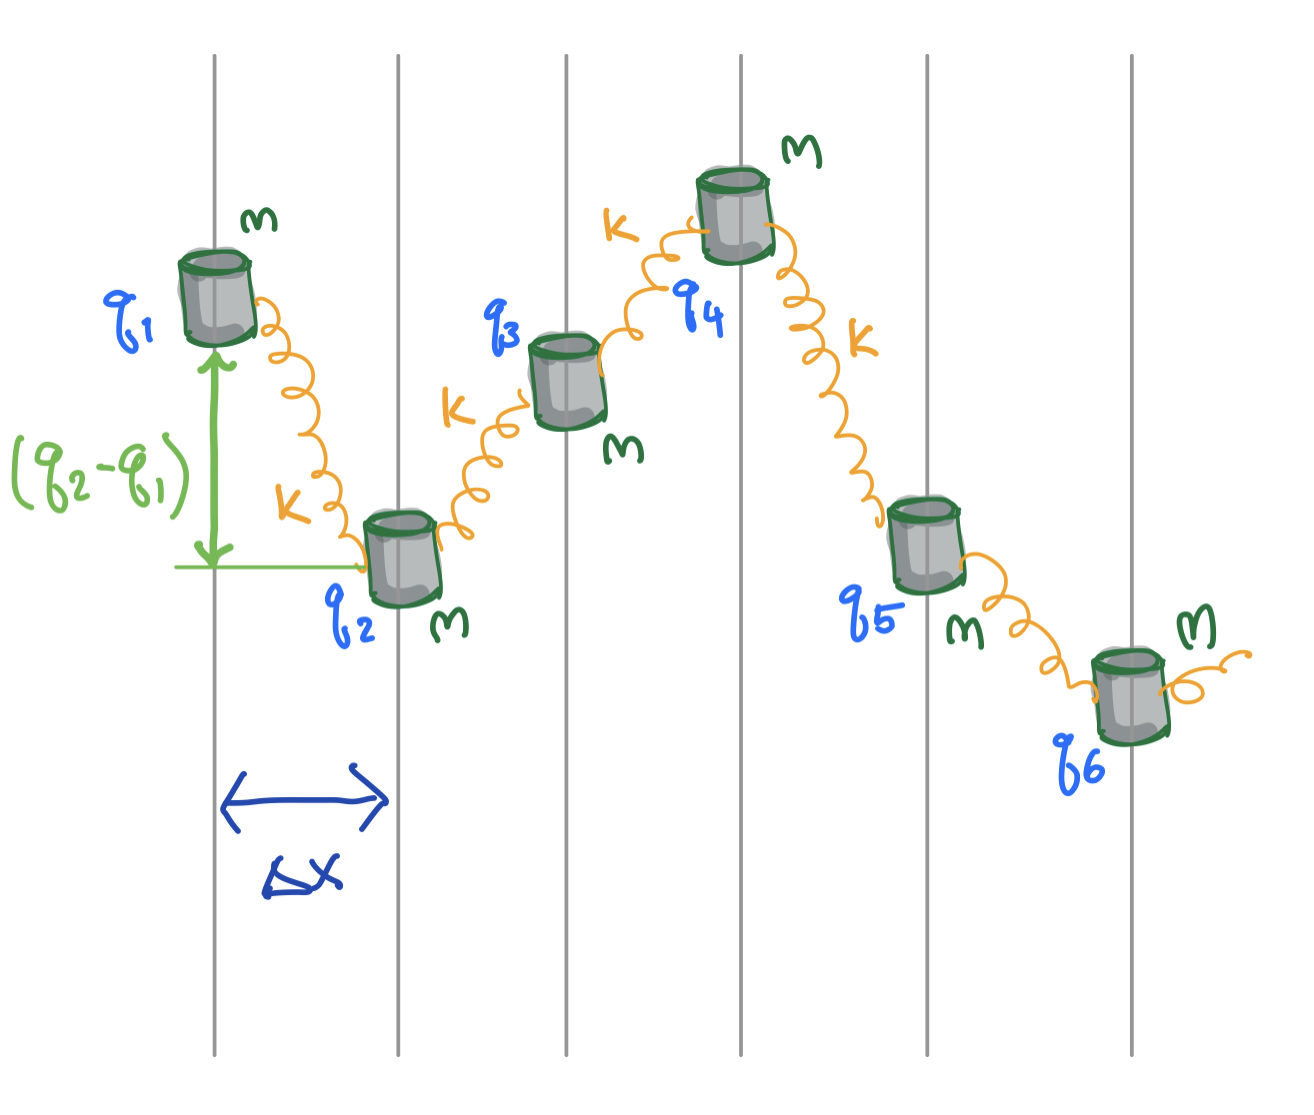
\includegraphics[width=.5\textwidth]{figures/coupledHO.jpg}
\end{center}
In the above picture we treated each value of $i$ as some point on a discretized spatial dimension. One could have equivalently treated $i$ as an index of a discretized time direction. In that way,
\begin{align}
	q_i \to q(t) \ ,
\end{align}
and the matrix/operator $A$ encodes something about propagation in time. For example, the harmonic oscillator would be $A \sim -(d/dt)^2$, where we take the appropriate discretized version of the second derivative:
\begin{align}
	A \sim 
	\begin{pmatrix}
	1 	& -2 & 1  &    &   &\\
		& 1  & -2 & 1  &   &\\
		&	 & 1  & -2 & 1 &\\
		&	&	&	&	& \ddots
	\end{pmatrix}
\end{align}
One can see clearly that $A$ couples nearby lattice points in time. If I displace the oscillator at time $i$, then at some later\footnote{One still has to impose causlity by hand since the operator is symmetric under time reversal.} time $j$ the oscillator will have some correlated displacement. In other words, the disturbance at time $i$ has \emph{propagated} to time $j$. The object that enabled that propagation is $A^{-1} \sim [-(d/dt)^2]^{-1} \sim G(t,t')$. 

Observe that even though $A$ is local---the discretized second derivative connects nearest-neighbors and next-to-nearest neighbor sites---the Green's function is \emph{non}-local: it allows the information to propagate over long distances. The physical mechanism is clear: if we think about this as a bunch of coupled oscillators (in time), then each oscillator causes its neighbor to move. You should imagine `the wave' in a stadium when the crowd cheers. As a matrix, the indices of the Green's function ($A^{-1}_{ij}$) gives the value of $q_j$ given a value at $q_i$:
\begin{center}
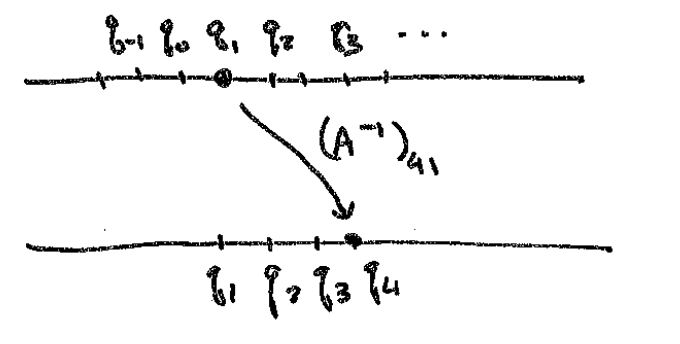
\includegraphics[width=.4\textwidth]{figures/P230b_2Ainv.png}
\end{center}
When we pass to the continuum limit, the product over $dq_1\cdots dq_N$ becomes a \emph{path integral} over all configurations in time:
\begin{align}
	\mathcal Dq(t) = dq_1\cdots dq_N \ .
\end{align}
The matrix multiplication turns into integrals
\begin{align}
	\vec{q}\vec{A}\vec{q} \to \int dt\, q(t) \left(-\frac{d^2}{dt^2} + \omega_9^2\right) q(t) \ ,
\end{align}
where you may want to take a moment to convince yourself that there's only one integral and not two. And, up to a factor of $i$, it looks like the 
\begin{align}
	Z[J=0] \sim \int \mathcal Dq(t) e^{i\int dt\, L} \ ,
\end{align}
where $L$ is the harmonic oscillator Lagrangian.


In fact, we can generalize even further and go from a particle propagating in time $q(t)$ to a field propagating in spacetime $q(x,t) = \varphi(x,t)$. We just have to imagine there being more indices. We can imagine $A$ becoming a tensor that acts as a `matrix' for each direction. I say `imagine' because it's a pain in the ass to actually write out, and it's better that we just imagine that one could do this: the point is that it is conceptually simple. 
In continuum language, $A$ is simply the quadratic part of the Lagrangian density:
\begin{align}
	A\to \partial^2 = \frac{1}{c^2} \frac{\partial^2}{\partial t^2} - \nabla^2 \ ,
\end{align}
and the generating function (which I usually just call a \emph{partition function} inspired by statistical physics) is
\begin{align}
	Z[J=0] &= \int \mathcal D\varphi(x,t) e^{iS[\varphi]} \ 
	&
	S[\varphi] &= \int d^4x \, \mathcal L \ ,
\end{align}
with $\mathcal L$ the Lagrangian \emph{density} for the theory. At this point, we can remind ourselves of \eqref{eq:G:QM}, throw in factors of $\hbar$ for dimensional consistency, and pat ourselves on the back. By the way, I don't think there's anything too deep to read into the fact that \eqref{eq:G:QM} is a quantum mechanical Green's function while $Z$ is a partition function. There's a slight nuance related to what is called second quantization (which is related to what we've been doing), but that is now beyond the focus of this course\footnote{See, e.g.~\url{https://sites.google.com/ucr.edu/p230b/}}.

\subsection{Interpretation}

What's the lesson of all of this? The `\emph{fields are coupled harmonic oscillators in spacetime}' picture gives us a lot of intuition for solving [linear] differential equations. It brings us to the \emph{origin} of these differential equations, the action. It connects the solution to the linear differential equations to a Gaussian integral. For the non-linear cases, we still need to do some work, but this is where life gets difficult. The coupled harmonic oscillator picture also brings us back to the notion of a \emph{discretized function space} as a crutch to understand the continuum\footnote{If you're a condensed matter physicist, then the lattice holds some physical significance. If you're a particle physicist, then you assume that the lattice is just a coarse model of the continuum. In either case, you gain a lot from working with a handful of fields rather than $N\to \infty$ coupled harmonic oscillators.}. That discrete function space picture helps reinforces the idea that the Green's function is the inverse of some quadratic form\footnote{This is the fancy way of saying matrix.} in the action. 

We develop some intuition for \emph{field theory} by placing \emph{sources} $J(x,t)$ on the lattice and taking functional derivatives with respect to them. This corresponds to imagining that there's some microscopic trouble-maker jumping up and down on one the harmonic oscillator at $\varphi(x,t)$ to create excitations of the field. The Green's function transmits these excitations to the rest of the lattice, according to the dynamics $\mathcal O \sim A$. Even though the dynamics are manifestly \emph{local} (derivatives $\sim$ nearest neighbor interactions), the Green's function is a \emph{propagator} that `exponentiates\footnote{At the level of this discussion, the word `exponentiates' is not a good choice. In quantum mechanics and the representation theory of groups, however, this is literally taking infinitesimal translations in spacetime, generated by e.g.~$\hat H$, and then creating a finite transformation by exponentiating it, $e^{-i\hat H t}$. In fact, in all of what we have done, the one picture that we have `missed' is the geometric one, which I keep referring to obliquely in footnotes like this. Sometimes the real story is in the footnotes (e.g.~the novel \emph{Pale Fire}).}' microscopic interactions into long-range interactions.

\paragraph{Big Picture.}
You now have the big picture the most common differential operators in physics. You'll have to slog through all sorts of second-order differential operators that are versions of the $\partial^2$ in different coordinate systems. Sometimes you'll have differential equations that are only single derivatives in time, and you'll know that this corresponds to a non-relativistic limit. You'll know that you won't find differential operators with only one power of $\nabla$ unless the system somehow breaks translation invariance. You'll have to solve these differential equations, usually by solving for the operators' Green's functions. You can do this in multiple ways; we reviewed the most popular methods in Section~\ref{sec:ways:to:solve:G}:
\begin{enumerate}

\item \textbf{Eigenfunctions and completeness}, Section~\ref{sec:Greens:fuctions:by:completeness}. Assuming one knows the eigenfunctions of the differential operator, this gives a series solution for the Green's function. It is practically useful only when the series is convergent.

\item \textbf{Patching}, Section~\ref{sec:patching}. This method assume that one can solve the \emph{homogeneous} differential equation $\mathcal O_x G(x,x')=0$ and then produces a piece-wise solution to the \emph{inhomogeneous} differential equation that defines the Green's function, $\mathcal O_x G(x,x')=\delta(x-x')$. This is practically useful in one dimension where the boundary conditions where the pieces are connected are easy to define.

\item \textbf{Fourier transform and its cousins}. This will be the topic of the rest of our course. We convert the differential equation into an \emph{algebraic equation} in momentum space. Aspects of the causal structure of the system that are manifested in complex momentum space. Furthermore, one can use contour integrals to do the `hard work.'
\end{enumerate}
When solving the Laplacian in different coordinates, you'll have to use different basis functions in place of the Fourier transform. You'll become good friends with the Bessel functions and spherical harmonics. They may look intimidating, but you'll remember that they're just a different basis for function space and they obey all the same nice features: they are orthonormal, they have real eigenvalues, and you can project functions onto that basis. The technical work you'll have to do will be cumbersome, but you will never be lost conceptually. You can always refer back to the simpler examples in this course.

The one thing that we didn't stress in this course is actually solving physical problems. We've brought you to the point where the solution $\psi(x)$ to a differential equation $\mathcal O_x \psi(x) = s(x)$ is
\begin{align}
	\psi(x) = \int dx'\, G(x,x')\, s(x') \ .
\end{align}
Actually \emph{doing} this integral is not interesting to me. It'll be interesting to you when the differential equation has some significance in your life (e.g.~a homework problem in electrodynamics). But this is just technical work. As far as I'm concerned, you could put that integral into \emph{Mathematica} or \emph{NumPy} and get the answer. Most of the physical intuition went into writing down that integral in the first place.

Great! We're now experts in solving linear differential equations. These correspond to the quadratic parts of the action and tend to be variants of the wave operator. However, you know from Section~\ref{sec:EFT:philosophy} that there are typically \emph{more} terms in the action than the quadratic part. For example, terms that go like $\varphi^3$ or $\varphi^4$ in the action give \emph{non-linear} differential equations, $\mathcal O_\text{quad}\varphi + \lambda \phi^3 = s$, for example. We even argued that it is precisely these non-linear terms that distinguish theories from one another: otherwise they all tend to be the \emph{same} second-derivative theory of non-interacting\footnote{We say non-interacting because the plane waves that pop out of the wave equation add linearly. This is obvious, right? The whole system was linear. The result is a theory which is completely solved, but rather uninteresting.} waves. The two approaches are (1) put everything on a computer and (2) appeal to perturbation theory with respect to the non-linear terms.
 

\section{Feynman Diagrams}

The idea of Feynman diagrams is to do perturbation theory with respect to the quadratic piece of the action. Rather then jumping into the field theory language, let's keep using the more familiar $N$-site lattice language. Let the matrix $A$ represent the quadratic part of the action which, at the very least, includes the kinetic term and the nearest-neighbor interactions. There is also the linear term, $\vec{J}\vec{q}$ that we interpret as a source for $\vec{q}$. Let us add to this a quartic term which we write as
\begin{align}
 	-V(\vec{q}) &= - \lambda \sum_i q_i^4 \ .
 \end{align}
The minus sign is to remind us that this is a potential term and such terms appear with a minus sign in the Lagrangian. $\lambda$ is a number that represents the four-point coupling or interaction strength. When $q_i$ is a discrete harmonic oscillator $\lambda$ has some dimension, but upon passing to the continuum field $\varphi$ using the normalization \eqref{eq:field:normalization} one can check that $\lambda$ is dimensionless in natural units. By the way, it is important that we wrote $\sum q_i^4$ and not $(\sum_i q_i)^4$. The latter mixes terms at different sites, whereas $q_i^4$ is a local term that is evaluated at each site $i$. 

The partition function/path integral/generating function for $\vec{q}$ in the presence of $V(\vec{q})$ is
\begin{align}
	Z_V[\vec{J}] &= \mathcal N^{-1} \int d^N\vec{q} \, 
		e^{-\frac{1}{2} \vec{qAq} + \vec{Jq} - V(\vec{q})}
		\\
	&= 
	\mathcal N^{-1} \int d^N\vec{q} \, 
	e^{-V\left(\frac{\partial}{\partial \vec{J}}\right)}
		e^{-\frac{1}{2} \vec{qAq} + \vec{Jq}} \ .
\end{align}
In the second line we have used the fact that because
\begin{align}
	\mathcal N^{-1} \int d^N\vec{q} \, 
	q_i^n \, 
	e^{-\frac{1}{2} \vec{qAq} + \vec{Jq}}
	=
	\mathcal N^{-1} \int d^N\vec{q} \, 
	\left(\frac{\partial}{\partial J_i}\right)^n
	e^{-\frac{1}{2} \vec{qAq} + \vec{Jq}} \ ,
\end{align}
one may write any function of $q_i$, including $e^{-V(\vec{q})}$ as a function of $(\partial/\partial J_i)$ acting on $Z[J]$, the generating function \emph{without} $V(\vec{q})$. Thus
\begin{align}
	Z_V[\vec{J}] &= e^{-V\left(\frac{\partial}{\partial \vec{J}}\right)} Z[\vec{J}] \ .
	\label{eq:ZV:from:Z}
\end{align}
It is conventional to write the generating function(al) to be a function of the source $\vec{J}$ since it is formally an integral transform of the distribution. When we take correlation functions, we take derivatives of $Z_V[\vec{J}]$ with respect to $\vec{J}$, recall \eqref{eq:correlator:J}.

As long as $\lambda$ is small, one may Taylor expand the exponential in $V(\vec{q})$,
\begin{align}
	Z_V[\vec{J}] &= Z[\vec{J}] + \lambda\left[-\sum_i \left(\frac{\partial}{\partial J_i}\right)^4\right] Z[\vec{J}] + \cdots \ .
\end{align}

Let's put this to work. Suppose I'd like to ask about the four-point correlation function between four oscillators, which I'll call $q_{1,2,3,4}$. I'm labeling them 1--4 for notational simplicity, not because they have to be sequential oscillators. You could have picked any four numbers, say $q_4$, $q_9$, $q_{8}$, and $q_{24}$. Mathematically, we know what this object corresponds to:
\begin{align}
	\langle q_1q_2q_3q_4 \rangle
	&= 
	\frac{1}{\mathcal N}
	\int d^N\vec{q} \, 
	q_1q_2q_3q_4 \,
	e^{-\frac{1}{2}\vec{qAq} - V(\vec{q})}
	\\
	&=
	\left.\frac{\partial^4 Z_V[\vec{J}]}{\partial J_1\partial J_2\partial J_3 \partial J_4}\right|_{\vec{J}=0}
	\\
	&= \left.\partial_{J_1}\partial_{J_2}\partial_{J_3}\partial_{J_4}
	\left(1 - \lambda\sum_i \partial_{J_i}^4 + \cdots\right) Z[\vec{J}] 
	\right|_{\vec{J}=0}
	\ .
	\label{eq:4pt:example:4derivatives}
\end{align}
At this point, let us recall the closed form expression for $Z[\vec{J}]$ from performing the Gaussian integral, \eqref{eq:Z:gaussian}:
\begin{align}
	Z[\vec{J}]
	=
	e^{\frac{1}{2}\vec{J}\vec{A}^{-1}\vec{J}} \ .
\end{align}
This means that
\begin{align}
	\left.
	\partial_{J_k}Z[\vec{J}]
	\right|_{\vec{J}=0}
	&= 
	\left(\vec{A}^{-1}\vec{J}\right)_k
	= 0
	&
	\left.
	\partial_{J_k}\partial_{J_\ell}Z[\vec{J}]
	\right|_{\vec{J}=0}
	&= 
	A^{-1}_{k\ell}
	\ .
\end{align}
This means that every \emph{pair} of derivatives with respect to source lattice sites $J_k$ and $J_\ell$ produces a propagator (Green's function) $A^{-1}_{k\ell}$. Any single derivative $\partial_{J_k}$ of $Z$ is proportional to $A^{-1}J$, which vanishes when we set the sources to zero. The $\mathcal O(\lambda^0)$ term of \eqref{eq:4pt:example:4derivatives} may be written as:
\begin{align}
	\left.
	\partial_{J_1}\partial_{J_2}\partial_{J_3}\partial_{J_4}
	Z[\vec{J}] 
	\right|_{\vec{J}=0}
	&=
	A^{-1}_{12}A^{-1}_{34} + A^{-1}_{13}A^{-1}_{24} + A^{-1}_{14}A^{-1}_{23} \ .
	\label{eq:4pt:ex:4der:leading:props}
\end{align}
The indices refer to particular lattice points where the sources are turned on. These, in turn, correspond to the specific oscillators int he correlation function $\langle q_1q_2q_3q_4 \rangle$. 
\begin{exercise}
Check that \eqref{eq:4pt:ex:4der:leading:props} is correct. You may need to do this the hard way and write out a bunch of terms to see how it works out. It is worth your time doing this to see how \eqref{eq:4pt:ex:4der:leading:props} pops out. 
\end{exercise}
There is a graphical way of drawing this. Assign each point $i=1,2,3,4$ a point on the page and draw $A^{-1}_{k\ell}$ as a line that connects point $k$ to point $\ell$. The result is
\begin{align}
	A^{-1}_{12}A^{-1}_{34} + A^{-1}_{13}A^{-1}_{24} + A^{-1}_{14}A^{-1}_{23} 
	&=
	\vcenter{
		\hbox{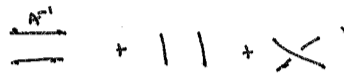
\includegraphics[width=.4\textwidth]{figures/P230b_4ptdisco.png}}
		} \ .
		\label{eq:feynman:4pt:disco}
\end{align}
The $\mathcal O(\lambda)$ term now has \emph{eight} derivatives with respect to $\vec{J}$; the four new ones are at some \emph{new} point $J_i$, which is then summed over: 
\begin{align}
	\left.
		- \lambda\sum_i
		\partial_{J_1}\partial_{J_2}\partial_{J_3}\partial_{J_4}
		 \partial_{J_i}^4
		Z[\vec{J}] 
	\right|_{\vec{J}=0} \ .
\end{align}
Following our observation above that pairs of $\partial_{J_k}\partial_{J_\ell}$ bring down a propagator $A^{-1}_{k\ell}$, we can write this diagrammatically in terms of a general intermediate point $i$ that is summed over:
\begin{align}
	\left.
		- \lambda\sum_i
		\partial_{J_1}\partial_{J_2}\partial_{J_3}\partial_{J_4}
		 \partial_{J_i}^4
		Z[\vec{J}] 
	\right|_{\vec{J}=0} 
	&=
	- 4! \lambda \sum_i
	A^{-1}_{1i} A^{-1}_{2i} A^{-1}_{3i} A^{-1}_{4i} \ .
\end{align}
The $4!$ is a combinatorial factor that counts the number of different ways in which you can pair up $J_i$ derivatives with $J_{1,2,3,4}$ derivatives. 
\begin{exercise}
Confirm the factor of $4!$ by explicitly deriving the above result.
\end{exercise}
Finally, we may write this diagrammatically as well:
\begin{align}
	- 4! \lambda \sum_i
	A^{-1}_{1i} A^{-1}_{2i} A^{-1}_{3i} A^{-1}_{4i}
	&= 
	\vcenter{
		\hbox{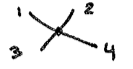
\includegraphics[width=.2\textwidth]{figures/P230b_4ptlocal.png}}
		}\ .
		\label{eq:feynman:4pt}
\end{align}
What we end up with is a rule for describing the Taylor expansion of $e^{-V[\partial_{\vec{J}}]}$ in \eqref{eq:ZV:from:Z} when calculating $n$-point correlation functions $\langle q_1\cdots q_n\rangle$:
\begin{enumerate}
\item For each of the $n$ points, draw a point on the page. Your goal will be the connect these points into a graph.

\item To leading order, connect all the points using lines that do not intersect. This represents free propagation and is the $\mathcal O(\lambda^0)$ contribution.

\item The $\mathcal O(\lambda)$ graphs correspond to the same set up, but with one additional point that accepts four lines. Draw all graphs where each point is connected, with the reminder that the new point must have four lines connecting to it.

\item You can read this graph as the product of propagators $A^{-1}_{k\ell}$ corresponding to each line. Each four-point vertex picks up a factor $\lambda$ (up to other combinatorial factors that one may determine).

\item For higher-order terms, you insert more vertices that accept four lines. One such vertex for each order in $\lambda$. You interpret more complicated diagrams the same way: each line corresponds to a propagator between those two nodes, each vertex comes with a prefactor of $\lambda$ up to combinatorial factors.
\end{enumerate}
As long as $\lambda$ is small, one may truncate the sum at a small number of insertions to approximate the correlation function. These are called Feynman diagrams.

\paragraph{Interpretation.}
Note that each line is a Green's function from the \emph{quadratic} operator $\vec{qAq}$: each line represents the solution to the \emph{linear} differential equation. Recall that this Green's function is precisely what `propagates' over long distances as a free wave. The vertices are the non-linearities. You can see this because rather than one $q$ coming in and one $q$ coming out, you have many $q$'s interacting at the same point. For example, you could read this as one $q$ turning into three lower-energy $q$s. This non-conservation of particle number for an interacting theory is part of what makes a quantum theory of fields different from quantum mechanics. 

By the way, the diagrams represent the \emph{dynamics} of a system. A rough definition of this is the physical content of the Lagrangian---how the states interact. This is in contrast to the \emph{kinematics} of the system, which has to do with things like the conservation of momentum  and dispersion-like relations (`on-shell-ness') that connect the energy of a state to its momentum. The diagrams tell you about possible [quantum] interactions, but you have to impose the phase space constraints before converting the diagrams into, say, a probability or a cross section.

The sum over all of these Feynman diagrams is completely analogous to the sum over histories in quantum mechanics. You can imagine that $q_1$ and $q_2$ are some harmonic oscillators in in the asymptotic past that have excitations. We would like to know the amplitude for those excitations to show up at harmonic oscillators $q_3$ and $q_4$ in the asymptotic future. In order to figure that out, we sum over all the ways in which those excitations could propagate. The leading terms include no interactions; this term is usually zero since you can't exchange momentum. The next-to-leading terms include an interaction where the initial particles overlap at a point $q_i$ before spitting out two new particles. In this way, you can `read off' a story of what the excitations are doing in spacetime. 

\paragraph{Connected versus disconnected.} The types of diagrams that we draw fall into two classes. There are disconnected diagrams like 
\eqref{eq:feynman:4pt:disco} and connected diagrams like \eqref{eq:feynman:4pt}. The disconnected diagrams represent propagation in spacetime, but not necessarily causal or kinematically allowed propagation. This is clear since each line is a propagator (Green's function, $A^{-1}$, $\cdots$). For a dynamical field, the propagator carries some well defined momentum. You know this because we know the propagator is the solution to a wave equation and so it's something like a sine wave with some well defined angular frequency (energy) and wave number (momentum).  If your initial and final states conserve total energy and momentum but are not otherwise identical, then the diagrams in \eqref{eq:feynman:4pt:disco} don't actually contribute. On the other hand, the four-point interaction in \eqref{eq:feynman:4pt} allows the states to exchange momenta. 

There's some good physics here. The standard introduction to field theory in statistical mechanics is the Ising model for magnetism: a lattice of spins that take binary values (spin-up or spin-down) with nearest-neighbor interactions. You may have already met this system: at high temperatures, the spins each have a lot of thermal energy and end up randomly oriented. At low temperatures, the dipole interactions between neighboring spins cause them to align. The typical length scale of these correlations are small---if you wiggle a spin at one lattice site, it's neighbor will respond, but the neighbor's neighbor may already be largely insensitive\footnote{This is just like in social situations: if you are blasting Rammstein at 3am in the morning, your next-door neighbors will get upset, but the people one apartment away will barely hear it.}. However, if one tunes the temperature to be near a \emph{critical temperature}, then the typical number of sites that are correlated becomes large: as if a wave is propagating across the lattice\footnote{This as if you played Rammstein at 3am in the morning, causing your neighbors to say `oh hell yes' and then turn on all of \emph{their} speakers up to also play Rammstein, and then \emph{their} neighbors do the same thing.}. I'll leave way in which this happens to your statistical mechanics/field theory courses, but suffice it to say that this is an example where a microphysical lattice has a continuum limit that is best described by a quantum field theory\footnote{What more, the quantum field theory exhibits universal behavior. It turns out to capture precisely the same physics as the water--ice transition.}. 


The connected and disconnected diagrams have a physical meaning in this system. Correlators like $\langle q_iq_j\rangle$ tell you how likely a spin at site $i$ is likely to be aligned with a spin at site $j$. If the temperature is near absolute zero, then this correlation is large no matter how far away $i$ and $j$ are: the thermal energy is so low that all of the spins want to line up. However, that's not really `propagation' of information: that's just the ground state of the system, reflected in the fact that the single-spin expectation value (``one-point correlation function,'' which sounds silly) is non-zero, $\langle q_i\rangle \approx \pm 1$. What we really care about is what happens when we flip one of the spins relative to that background. Thus the figure of merit is the \emph{connected} two-point function:
\begin{align}
	\langle q_i q_j\rangle_\text{connected} = \langle q_i q_j\rangle 
	- \langle q_i\rangle\langle q_j\rangle \ ,
\end{align}
where the second term removes the effect of the ground state being aligned. As you can expect from its name, the connected correlation function only includes diagrams that are connected. In a particle-physics-based field theory course, one usually sees the removal of disconnected diagrams when carefully normalizing the partition function\footnote{By the way, in the discussion above I did \emph{not} carefully normalize the partition function. The value of $\mathcal N$ should be with respect to the full theory, not just the free theory. However, we didn't actually use this normalization so it was convenient to lie a bit for pedagogical efficiency.}. Here it's nice to have a concrete physical interpretation.


\paragraph{Onward and upward.}
Now you know everything you need to know to play with Feynman diagrams\footnote{See, e.g.~\url{https://sites.google.com/ucr.edu/p165/}. For a teaser, you can try this exercise that I give to the undergraduate particle physics course: \url{https://github.com/Tanedo/Physics165-2020/blob/master/P165_L02.pdf}.}.








 





% Connected: https://www.youtube.com/watch?v=7WaBFvjk06w
% Then: do bayes
% Tenn: do Kramers Kronig












\section{Closing Thoughts}

What I hope you've come to appreciate is that the mathematical machinery that you face in your first year of graduate school may appear daunting at first, but that you're never too far off from some variation of the harmonic oscillator. Green's functions are a powerful tool for solving differential equations, but we found that their \emph{analytic structure} tells is about the underlying physics of our theory. We waxed poetic about going from a harmonic oscillator to a field and how this is connected to the idea of extending time to spacetime. We danced carefully with the picture of functions as infinite-dimensional function spaces that could be understood in their discretized form as large-but-finite-dimensional vector spaces. We said a few words about the notion of effective theory and action principles. After arguing that everything really does reduce to something like a harmonic oscillator, we showed one way (perturbation theory) to deal with the \emph{non-linearities} that make \emph{actual} physics really interesting. There are any number of directions for you to go from here. Experimentalists and observers may want to dig into statistics and probability, condensed matter folks may flock to statistical mechanics while particle folks head to quantum field theory (only to discover that at the hearts of their respective fields they are speaking dialects of the same language\footnote{... that differ by an $i$}). From here on out, \emph{you} define your path through mathematical physics: what you need for your work, what tickles your fancy, and what gets a slice of your precious attention as you set forth in your scientific careers.



\section*{Acknowledgments}
%This work is supported in part by 
%the \textsc{nsf} grant \textsc{phy}-1316792. 
%
I thank the students of Physics 231 (2016--2020) for their patience and feedback on on this course. Especially notable are those poor souls who suffered the first iteration of this course in 2016. I appreciate the advice of my more experienced colleagues when shaping this course and the many fantastic physics references out there that each take their own twists through mathematical physics. I am especially appreciative to the textbooks by Stone and Goldbart as well as that by Cahill. Those two references not only inspired big portions of these notes, but also led me down hours of delightful rabbit holes of enlightenment that did not necessarily end up in my course.

\appendix
\input{Lec-999-Appendix-method-of-variations}
\input{Lec-0A-Fourier}
%!TEX root = P231_notes.tex
%% From: 2917 Lec 22 and onward
\section{Nuts and Bolts Probability}
\label{sec:probability}

Let's forget Green's functions now and follow up on something to do with probability: Bayes' theorem. This is fully outside the scope of the class, but it is significant enough that it deserves to be mentioned in a `math methods' course. 

You are already familiar with \emph{conditional probability}. If you roll two 6-sided dice, the probability of each coming up with one is simply the product of each probability:
\begin{align}
	P(\text{both dice are 1}) = P(\text{one die is 1})^2 \ .
\end{align}
In this case we're asking about two events, $A$ (first die rolls 1) and $B$ (second die rolls 1). In general, though, these two events may not be independent. In this case, one has to deal with \emph{conditional probability}. We write $P(A|B)$ to mean the probability of $A$ assuming that $B$ is true. This, in turn, is related to the probability that $A$ \emph{and} $B$ are true divided by the probability that $B$ is true:
\begin{align}
	P(A|B) &= \frac{P(A\& B)}{P(B)} \ .
	\label{eq:P:A:given:B}
\end{align}
Stop to make sure this makes sense: if you write the probabilities as
\begin{align}
	P(X) = \frac{\text{number of times $X$ happens}}{\text{total number of samples}} \ ,
\end{align}
then the right-hand side of \eqref{eq:P:A:given:B} is simply
\begin{align}
	P(A|B) = \frac{\text{number of times $A$ and $B$ happen}}{\text{number of times $B$ happens}} \ , 
\end{align}
which is precisely what we want from $P(A|B)$: what is the probability that $A$ is true if we already know $B$ is true. Once we say $B$ is true, we can throw away all the samples where $B$ is not true.

Here's the key insight: $P(A|B)P(B) = P(A\& B)$. On the right hand side, $A\&B$ is completely symmetric in $A$ and $B$. That means we could swap them on the left-hand side as well: 
\begin{align}
	P(A\&B) = P(B\& A) = P(B|A)P(A) \ . 
\end{align}
We thus have $P(A|B)P(B)=P(B|A)P(A)$, which gives us the famous \textbf{Bayes theorem} that relates the conditional probabilities $P(A|B)$ and $P(B|A)$:
\begin{align}
	P(A|B) &= \frac{P(B|A) P(A)}{P(B)} \ .
\end{align}
Here's a useful graphical representation from Bob Cousins:
\begin{center}
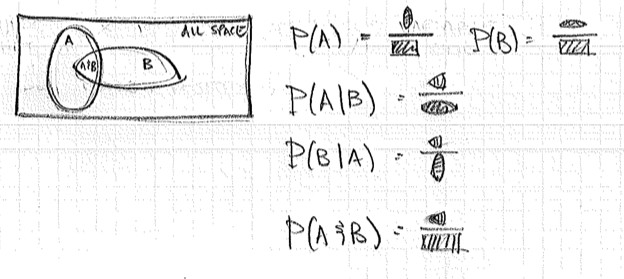
\includegraphics[width=.8\textwidth]{figures/ConditionalProb.png}
\end{center}
What is important here is that $P(A|B)$ and $P(B|A)$ can differ significantly if $P(A)/P(B)$ is very big or very small. This can be problematic because human beings can be sloppy when distinguishing $A|B$ versus $B|A$. 
\begin{example}
The probability that someone knows how to use \texttt{ROOT}\footnote{\url{https://root.cern/}} given that they are a particle physicist is roughly $P(\text{\texttt{ROOT}}|\text{particle person}) \approx 50\%$. To rough approximation, particle experimentalists use \texttt{ROOT} and theorists avoid it like the plague. However, the probability that someone is a particle physicist given that they use \texttt{ROOT} is $P(\text{particle person}|\text{\texttt{ROOT}}) \approx 100\%$. If someone uses \texttt{ROOT}, then you can be pretty sure that they do particle physics.
\end{example}

There's a simple reason why this is important: usually $A$ is something that we can actually see and $B$ is something that we want to \emph{infer} but cannot directly test. Specifically, in physics we typically have the following case:
\begin{align}
	A &= \text{data} 
	&
	B &= \text{theory} \ .
\end{align}
$A$ is the particular data that an experimentalist or an observer actually records. $B$ roughly a statement about whether a theory is correct. 
% 
We've already made may caveats in Section~\ref{sec:EFT:philosophy} about the idea of effective theories and what it means for a theory to be `correct.' To summarize, usually $B$ is asking: is a given theory a good description of the underlying phenomenon related to the data $A$? 

At this point, I'll leave it to you to dig deeper into the formalism for probabilities\footnote{Some of my favorite references: \emph{Statistics: A Guide to the Use of Statistical Methods in the Physical Sciences}, the lectures by Bob Cousins \texttt{1807.05996} (and his 1995 \emph{American Journal of Physics} article), and Kyle Cranmer's statistics and data science textbook~\url{https://cranmer.github.io/stats-ds-book/}.}. In summary, you should be precise about your hypothesis tests and be able to clearly articulate the meaning of whatever figure of merit you're using to interpret your data. In what follows, let's just play with some silly manifestation of these ideas. 

\subsection{Were we lucky that the LHC didn't destroy the world?}
\label{sec:LHC:luck}

One of the favorite discussion topics when I was a graduate student was a funny clip from \emph{The Daily Show} about the Large Hadron Collider in 2009\footnote{\url{http://www.cc.com/video-clips/hzqmb9/the-daily-show-with-jon-stewart-large-hadron-collider}}
. At the time, there was speculation that the LHC could destroy the world. There were many fun and silly ideas for how this could come about, though there were many very good reasons why these ideas were more `silly science fiction' rather than environmental concern\footnote{\url{https://home.cern/science/accelerators/large-hadron-collider/safety-lhc}}. During the clip, John Oliver---then a correspondent for John Stewart's \emph{The Daily Show}---interviews some dude concerned about the possibility that the \acro{LHC} may destroy the world. The interview went something like this:
\begin{quote}
\textsc{Oliver}: What are the chances that the world is going to be destroyed?\\
\textsc{Dude}: It's about a one in two chance.\\
\textsc{Oliver}: 50--50?\\
\textsc{Dude}: It's either going to happen or not happen. So the best guess is 50--50.
\end{quote}
\begin{exercise}
What's wrong with that dude's argument?
\end{exercise}
 

\subsection{The Prosecutor's Fallacy}


This comes from Bergstrom and West's book \emph{Calling Bullshit}. Imagine some high-profile \emph{Ocean's Eleven} or \emph{Carmen Sandiego} style heist. The \acro{FBI} is able to recover a set of fingerprints which they run through their database of 50 million people and guess what: \emph{you're} a match. Against everyone's advice, you decide to represent yourself in court. When the \acro{FBI} agent explains that your fingerprint match makes is an open-and-shut case, you politely ask: \emph{what is the chance that the wrong fingerprint would be matched with a print in the database?}

``Hah!'' the prosecutor scoffs at you. ``The chance of this happening happens to be \emph{one in ten million}. That's beyond any reasonable doubt.'' Fortunately you know a thing or two about probability and there's a chalkboard in the courtroom. You draw the following table:
\begin{center}
\begin{tabular}{l|ll} \toprule % @{} removes space
		& Match & No Match
		\\ \hline
		Guilty & \phantom{1 person} & \phantom{0 people}
		\\
		Innocent & \phantom{5 person} & \phantom{50,000,000 people}
		\\ \bottomrule
\end{tabular}
\end{center}
You start by stating the obvious assumptions. There is \emph{one} guilty person---not you---whose fingerprints match the prints lifted from the crime scene. While it's neither here nor there, you also point out that there are no people who are both guilty but whose prints do not match those at the crime scene. You start to fill in the table:
\begin{center}
\begin{tabular}{l|ll} \toprule % @{} removes space
		& Match & No Match
		\\ \hline
		Guilty & {1 person} & {0 people}
		\\
		Innocent & \phantom{5 person} & \phantom{50,000,000 people}
		\\ \bottomrule
\end{tabular}
\end{center}
Next you say that there are approximately 50 million people in the fingerprint database. Almost all of theme are innocent and almost all of them are completely distinct from the evidence from the crime scene. You fill in the table a bit more:
\begin{center}
\begin{tabular}{l|ll} \toprule % @{} removes space
		& Match & No Match
		\\ \hline
		Guilty & {1 person} & {0 people}
		\\
		Innocent & \phantom{5 person} & {50,000,000 people}
		\\ \bottomrule
\end{tabular}
\end{center}
Finally, you point out: given a false-match rate of one in 10 million, you can estimate that around \emph{five} innocent people will have fingerprints that match those at the crime scene. 
\begin{center}
\begin{tabular}{l|ll} \toprule % @{} removes space
		& Match & No Match
		\\ \hline
		Guilty & {1 person} & {0 people}
		\\
		Innocent & {5 person} & {50,000,000 people}
		\\ \bottomrule
\end{tabular}
\end{center}
The prosecutor starts to sweat, they can see what's coming. You point out that the \emph{data} in the case is that you are one person whose fingerprints match those at the crime scene. That means we should focus only on the population of people whose fingerprints match those the crime scene: there are approximately six: five innocent and one guilty. You point to the numbers and say, ``I know that my \emph{Math Methods} class in graduate school wasn't \emph{especially} rigorous, but clearly there is a five in six chance that even though my fingerprint matches the one from the crime scene, I am in fact innocent.''
\begin{exercise}
What was the mistake that the prosecutor made?
\end{exercise}
Bergstrom and West made up the above story to explain the fallacy, but they point out that this scenario indeed played out in 2018 in the highly publicized case that led to the capture of the Golden State Killer using \acro{DNA} samples from a genealogy company. What was not shared widely in the press coverage was that the genetic screening alone initially led to the \emph{wrong} suspect. The true culprit was identified by combining the \acro{DNA} match with other evidence from more traditional detective work.

\subsection{Why we are not evidence for God}

Mathematician Jordan Ellenberg takes the above example a bit further to highlight another fallacy. This comes from his pop mathematics book \emph{How Not To Be Wrong}, which you're probably a bit advanced for, but is none-the-less a fun read and a lesson in effective technical communication to a lay audience. 

There is an argument that the universe we observe is evidence for God. After all, look how incredibly engineered and fine-tuned life is\footnote{You can also point to more physical arguments, like the apparent fine tuning of the cosmological constant.}. Indeed all this \emph{stuff} that we see around us does seem rather complicated---why isn't the universe more like the spherical cow\footnote{\url{https://en.wikipedia.org/wiki/Spherical_cow}} theories that we study in grad school? 

The argument is something like the one in Appendix~\ref{sec:LHC:luck}. Let's write down the \emph{likelihood} that we see this complicated universe. Ellenberg makes some very rough estimates that will be sufficient for our point. The existence of an omnipotent creator could seems to be far more likely to have created such a finely-tuned, complicated universe.
\begin{center}
\begin{tabular}{l|ll} \toprule % @{} removes space
		& God Exists & No God
		\\ \hline
		Simple universe &  & 
		\\
		Complicated universe & $10^{-6}$  & $10^{-18}$
		\\ \bottomrule
\end{tabular}
\end{center}
We don't bother to write out the first row---after all, that's not the case we care about. There you have it: it seems like the observation that our universe is complicated gives overwhelming evidence that God exists. 

Of course, the problem is that we have \emph{assumed} that God exists and God doesn't exist are the only possible outcomes. This is analogous to assuming that you have a theory for an exotic new particle and the results of an experiment either rejects existence of the exotic new particle in favor of the null hypothesis (no new particles) or confirms the existence of the exotic new particle (alternate hypothesis). You know this is too na\"ive. Sometimes there are other reasons why the data of your experiment looks funny---maybe you didn't plug in your cables properly\footnote{\url{https://en.wikipedia.org/wiki/Faster-than-light_neutrino_anomaly}}. So in our ontological argument, Ellenberg says that we should be sure to consider all possibilities. For example, often times complicated things come about by the dreaded `design by committee.' So maybe it's not that God exists, but that there's a whole pantheon of gods who designed the universe through a complex process of peer review and feedback. The result is \emph{this} ugly mess. Our table now looks like
\begin{center}
\begin{tabular}{l|lll} \toprule % @{} removes space
		& God Exists & No God & Many Gods
		\\ \hline
		Simple universe &  & &
		\\
		Complicated universe & $10^{-6}$  & $10^{-18}$ & $10^{-5}$
		\\ \bottomrule
\end{tabular}
\end{center}
The number we threw in here is fairly arbitrary, but the point is that you could make the argument that \emph{many gods} may be more likely than \emph{one god}. Fine, but for a physics class this is starting to look a little bit too much like religious studies, no? Well, as we ponder the origin of our universe, we go to knock on the door of our cosmology colleagues, only to find that they're busy running their cosmological simulation. Aha! You remember playing \emph{The Sims}, which is an odd knock-off experience compared to actual real life. However, it seems plausible that a sufficiently advanced civilization would have created a computer game to simulate their existence. Perhaps when that simulated reality is sufficiently advanced, it too will create a computer program that simulates \emph{their} reality. And so forth. You start to think that this, too, is a rather plausible origin for a strangely complicated universe. Ellenberg updates our table as follows
\begin{center}
\begin{tabular}{l|llll} \toprule % @{} removes space
		& God Exists & No God & Many Gods & Simulated reality
		\\ \hline
		Simple universe &  & & &
		\\
		Complicated universe & $10^{-6}$  & $10^{-18}$ & $10^{-5}$ & $10^{-1}$
		\\ \bottomrule
\end{tabular}
\end{center}
At the level of this crude example, it seems that the most likely possibility is that not only does any god \emph{not} exist, but it's unlikely that we exist. 

\subsection{The End of the World}

There's a cute example of Bayesian statistics that I read about in William Poundstone's \emph{The Doomsday Calculation.} I had the pleasure of meeting William Poundstone once and he seems like a nice and intelligent person. Unfortunately, I did not much enjoy the book. You can read the main argument in Poundstone's article for \emph{Vox}\footnote{\url{https://www.vox.com/the-highlight/2019/6/28/18760585/doomsday-argument-calculation-prediction-j-richard-gott}}.

The example comes from Richard Gott, a renowned astrophysicist. Gott visited the Berlin wall in the summer of 1969. The Berlin wall was built in 1961, so by then the wall was $t=8$ years old. Gott claims to have wondered how long the Berlin wall would stand and came up with the following argument.

Gott figured that there was nothing special about him visiting the Berlin wall in 1969. Assuming that the Berlin wall would be torn down, it had a finite lifetime $T$. He just happened to sample the existence of the Berlin wall at some moment of time within that lifetime. He assumed was no reason for him to be visiting the wall particularly early or particularly late in its lifetime; thus, there's a uniform `prior' probability that he'd visit the wall at any time during its lifetime. With this assumption, he said that there's a 50\% chance that his visit in 1969 happens to fall within the middle 50\% interval of $T$. In other words, there's a 50\% chance that $t=8$ is somewhere between $.25\times T$ and $.75\times T$. 
\begin{itemize}
\item If $t=8$ corresponds to $0.25 \times T$---that is, he happened to show up a little \emph{early} in the wall's lifetime---then $T=32$ and the wall would stand for another 24 years. 

\item Alternatively, if $t=8$ to $0.75 \times T$---that is, he happened to show up a little \emph{late} in the wall's lifetime---then $T=10.6$ and the wall would stand for only another 2.6 years. 
\end{itemize}
This brackets an anticipated lifetime for the Berlin wall to be between $T=10.6$ and $T=32$ years, or a range of dates 1972--1993. Spoiler alert: the Berlin wall was torn down in 1989, which is indeed in this range of years. 

Gott went on to speculate about the implications on how long humanity would survive\footnote{\url{https://www.nature.com/articles/363315a0.epdf}}.
\begin{exercise}
Using Gott's technique for estimating the lifespan of the Berlin wall and the approximation that humanity has existed for around 200,000 years, what is a plausible range of lifetimes for human existence?
\end{exercise}



%
% \textsc{p.t.} thanks the Aspen Center for Physics (NSF grant \#1066293) for its hospitality during a period where part of this work was completed. \textsc{p.t.} is supported by the DOE grant \textsc{de-sc}/0008541.

%% Appendices
% \appendix


%% Bibliography
%\bibliographystyle{utcaps} 	% arXiv hyperlinks, preserves caps in title
%\bibliographystyle{utphys} 	% arXiv hyperlinks
% \bibliography{bib title without .bib}


\end{document}